%\documentclass[newPxFont]{beamer}
%\usetheme{sthlm}
%\documentclass[slidestop,compress,11pt,xcolor=dvipsnames,aspectratio=169]{beamer}
\documentclass[slidestop,compress,11pt,xcolor=dvipsnames]{beamer}
\usepackage[bars]{beamerthemetree} % Beamer theme v 2.2
\usepackage[fontsize=8]{pdfcomment}
\usepackage{colortbl}
\usepackage{multirow}
\usepackage{kerkis}
\usepackage{media9}

\mode<presentation> {
\usefonttheme[onlymath]{serif}
\usetheme{Ilmenau}
\setbeamertemplate{navigation symbols}{} % To remove the navigation symbols from the bottom of all slides uncomment this line
\useinnertheme{circles} %rectangle bullet points instead of circle ones
\useoutertheme[subsection=false]{smoothbars}%Beamer Outer Theme-circles on top
%\setbeamertemplate{footline}[frame number]
}
\newcommand*\oldmacro{}%
\let\oldmacro\insertshorttitle%
\renewcommand*\insertshorttitle{%
\oldmacro\hfill%
\insertframenumber\,}%/\,\inserttotalframenumber

% Creates a slide with the name of the section
%\AtBeginSection[]{
%  \begin{frame}
%  \vfill
%  \centering
%  \begin{beamercolorbox}[sep=8pt,center,shadow=true,rounded=true]{title}
%    \usebeamerfont{title}\insertsectionhead\par%
%  \end{beamercolorbox}
%  \vfill
%  \end{frame}
%}
\graphicspath{{images/}}

%\titlegraphic{
\includegraphics[height=.15\textheight]{logo/fapesp_s}}
\titlegraphic{

\includegraphics[height=.10\textheight]{logo/fapesp_s}
\hspace{1cm}

\includegraphics[height=.08\textheight]{logo/usp}
%\hspace{2cm}
%
\includegraphics[width=1.5cm]{logo/fmrp}
%\hspace{1cm}
}
\usepackage{csvsimple}
\usepackage{multicol}
\usepackage{remreset}% tiny package containing just the \@removefromreset command
\makeatletter
\@removefromreset{subsection}{section}
\makeatother
\setcounter{subsection}{1}


\usepackage{tikz}
\usetikzlibrary{shadings}

\colorlet{titleleft}{black}
\colorlet{titlemiddle}{blue!20!black}
\colorlet{titleright}{blue!40!black}

\pgfdeclarehorizontalshading[titleleft,titlemiddle,titleright]      {beamer@frametitleshade}{\paperheight}{%
    color(0\paperwidth)=(titleleft);
    color(0.15\paperwidth)=(titleleft);
  color(0.5\paperwidth)=(titlemiddle);
  color(0.85\paperwidth)=(titleright);
  color(\paperwidth)=(titleright)
}

\makeatletter

\setbeamertemplate{footline}
{
    \leavevmode%
    \setbox\beamer@tempbox=\hbox{%
        \begin{beamercolorbox}[wd=.233333\paperwidth,ht=3.0ex,sep=1ex,center]{parent=palette tertiary,bg=,fg=white}%
            \color{white}{RECOMB-CBB | Tiago C. Silva} \expandafter\beamer@ifempty\expandafter{\beamer@shortinstitute}{}{~~(\insertshortinstitute)}
        \end{beamercolorbox}%
        \begin{beamercolorbox}[wd=.533333\paperwidth,ht=3.0ex,sep=1ex,center]{parent=palette secondary,bg=,fg=white}%
             \color{white}{\usebeamerfont{title in head/foot}
            \textit{ELMER} v.2: Enhancer Linking by Methylation/Expression Relationship 
             }
        \end{beamercolorbox}%
        \begin{beamercolorbox}[wd=.233333\paperwidth,ht=3.0ex,sep=1ex,right]{parent=palette primary,bg=,fg=white}%
         \color{white}{
            \usebeamerfont{date in head/foot}\insertshortdate{}\hspace*{2em}
            \insertframenumber{} / \inserttotalframenumber\hspace*{2ex} 
            }
        \end{beamercolorbox}%
        }%
        \vskip-\beamer@tempdim%
        \beamer@tempdim=\ht\beamer@tempbox%
        \advance\beamer@tempdim by 4pt%
        \begin{pgfpicture}{0pt}{0pt}{\paperwidth}{20pt}
            \pgfpathrectangle{\pgfpointorigin}{\pgfpoint{\paperwidth}{\beamer@tempdim}}
            \pgfusepath{clip}
            \pgftext[left,base]{\pgfuseshading{beamer@frametitleshade}}
        \end{pgfpicture}
        \vskip-\beamer@tempdim%
        \box\beamer@tempbox%    
}%
\makeatother

\usepackage{csvsimple}
\usepackage{siunitx}
\usepackage{float}
\usepackage{booktabs}
\usepackage{tikz}

\usepackage{caption}
\captionsetup{font=scriptsize,labelfont=scriptsize}

%-=-=-=-=-=-=-=-=-=-=-=-=-=-=-=-=-=-=-=-=-=-=-=-=
%        LOADING PACKAGES
%-=-=-=-=-=-=-=-=-=-=-=-=-=-=-=-=-=-=-=-=-=-=-=-=
\usepackage[utf8]{inputenc}

%-=-=-=-=-=-=-=-=-=-=-=-=-=-=-=-=-=-=-=-=-=-=-=-=
%        BEAMER OPTIONS
%-=-=-=-=-=-=-=-=-=-=-=-=-=-=-=-=-=-=-=-=-=-=-=-=

%\setbeameroption{show notes}

%-=-=-=-=-=-=-=-=-=-=-=-=-=-=-=-=-=-=-=-=-=-=-=-=
%
%	PRESENTATION INFORMATION
%
%-=-=-=-=-=-=-=-=-=-=-=-=-=-=-=-=-=-=-=-=-=-=-=-=

\title{ELMER v2}
\subtitle{An R/Bioconductor package to reconstruct gene regulatory networks from DNA methylation and transcriptome profiles}
%\date{\small{\jobname}}
\date{\today}
\author[Tiago Chedraoui Silva]{\texttt {Tiago Chedraoui Silva}\\ \texttt{RECOMB-CBB}} % auteur
%\author{\texttt{Tiago Chedraoui Silva}}
\institute{University of São Paulo / Cedar-Sinai }

\begin{document}

%-=-=-=-=-=-=-=-=-=-=-=-=-=-=-=-=-=-=-=-=-=-=-=-=
%
%	TITLE PAGE
%
%-=-=-=-=-=-=-=-=-=-=-=-=-=-=-=-=-=-=-=-=-=-=-=-=

{
\setbeamertemplate{footline}{}
\maketitle
}
%\begin{frame}[plain]
%	\titlepage
%\end{frame}


\section*{Overview}
\begin{frame}{Overview}
\begin{enumerate}
\setlength\itemsep{2em}
\item Introduction
\item Objectives
\item Methods: Algorithms and tools
\item Analysis
\item Conclusion
\end{enumerate}
 % For longer presentations use hideallsubsections option
 %\tableofcontents[hideallsubsections]
\end{frame}


%-=-=-=-=-=-=-=-=-=-=-=-=-=-=-=-=-=-=-=-=-=-=-=-=
%
%	SECTION: BACKGROUND
%
%-=-=-=-=-=-=-=-=-=-=-=-=-=-=-=-=-=-=-=-=-=-=-=-=

\section{Introduction}

\begin{frame}{Enhancer-mediated gene regulation}
 \vspace*{1.0cm}
 \begin{figure}
  \centering
  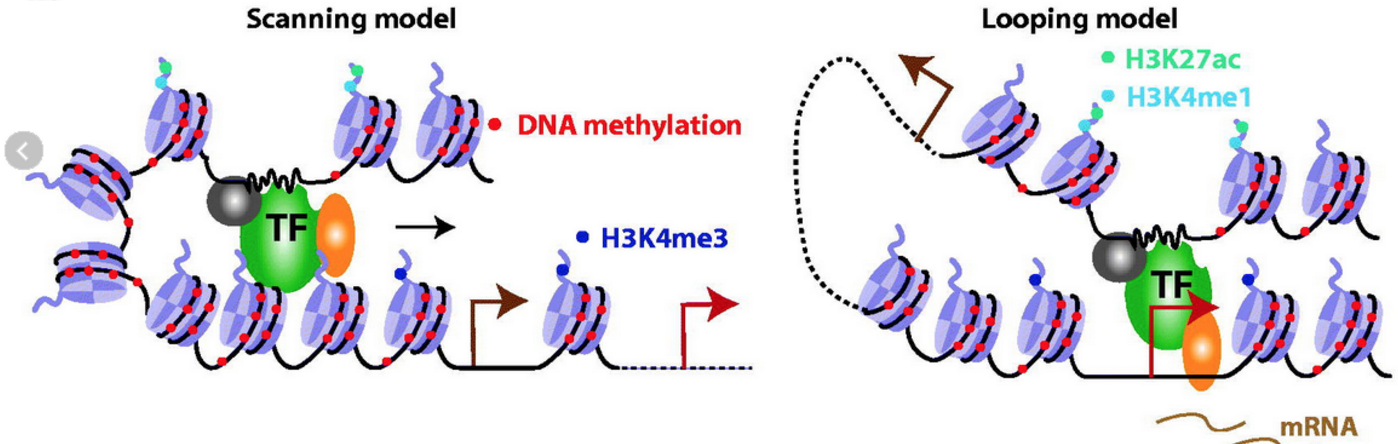
\includegraphics[width=1.0\linewidth]{ELMER/elmer.png}{\tiny{\\\href{https://genomebiology.biomedcentral.com/articles/10.1186/s13059-015-0668-3}{Source: Yao et al. Genome Biology (2015)}}}
 \end{figure}
\end{frame}

% Shown are two models for gene regulation by enhancers. The left panel illustrates the ?scanning or tracking? model in which a transcription factor (TF)-containing protein complex binds at an enhancer and moves along the genome, searching for a target promoter (the nearest promoters are labeled in brown and distal promoters are labeled in red). 
% The right panel illustrates the ?looping? model in which an enhancer directly interacts with a target promoter by forming a DNA loop mediated by protein?protein contacts


\begin{frame}{Enhancer-mediated gene regulation}
 \begin{itemize}
  \item 73\% of the tested distal elements do not link to the nearest gene (Sanyal et al., 2012)
  \item 40\% of the enhancers involved in loops do not interact with the TSS of the nearest gene (Li et al., 2012),
  \item one-third of the distal interactions were not directed to the promoter of the nearest gene (Mifsud et al., 2015),
  \item 85\% of tumor-specific enhancers that could be linked to the expression of a nearby gene skipped the nearest gene (Yao et al., 2015).
 \end{itemize}
\end{frame}

\begin{frame}{Enhancer-mediated gene regulation}
 \vspace*{-0.1cm}
 \begin{figure}
  \centering
  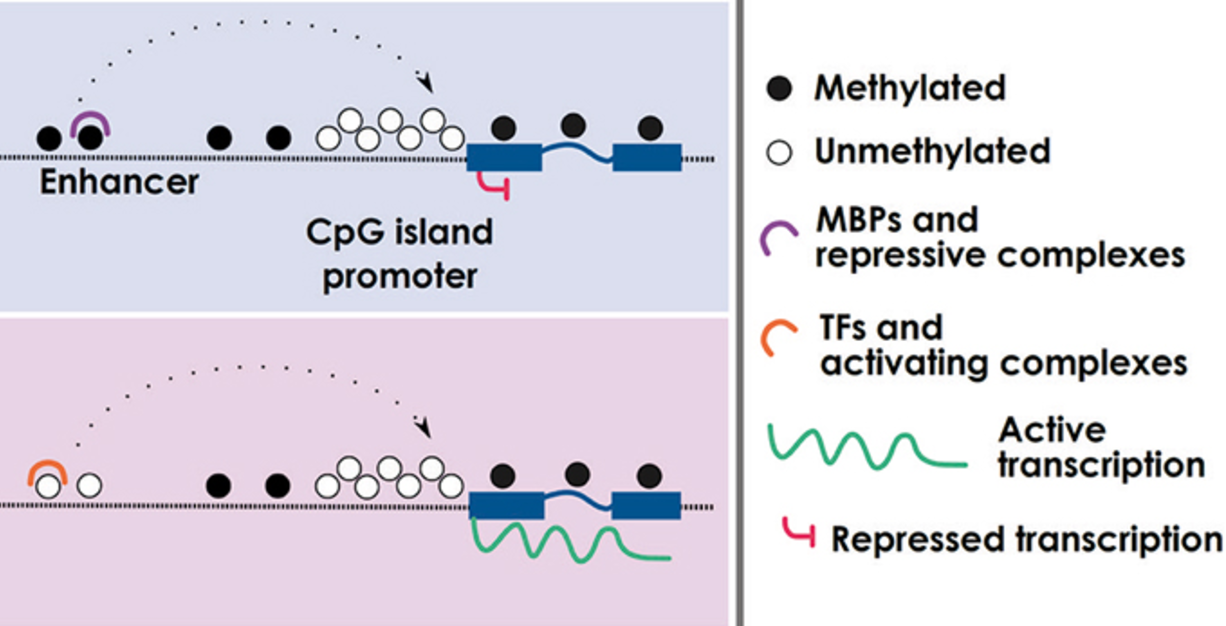
\includegraphics[width=1.0\linewidth]{ELMER/dna_met.png}{\tiny{\\Source: Carrio et al. Frontiers in aging neuroscience (2015)}}
 \end{figure}
\end{frame}


\section{ELMER}
\begin{frame}{\normalsize{ELMER v.2:  Enhancer Linking by Methylation/Expression Relationship}}
 \begin{figure}
  \centering
  \includegraphics[width=1.0\linewidth]{ELMER/painel_A.pdf} \end{figure}
\end{frame}


\begin{frame}{Algorithm}

\begin{exampleblock}{Steps}
\begin{enumerate}
\item  Identify distal probes on HM450K/EPIC.
\item  Identify distal probes with significantly different DNA methylation level in  group 1 compared to group 2.
\item  Identify putative target genes for differentially methylated distal enhancer probes.
\item  Identify enriched motifs for the distal  probes which are significantly differentially methylated and linked to a putative target gene.
\item  Identify regulatory TFs whose expression associate with DNA methylation at motifs.
\end{enumerate}

\end{exampleblock}
\end{frame}


\begin{frame}{Step 1: Identify distal probes}
 %\vspace*{1.0cm}
 \begin{figure}
  \centering
  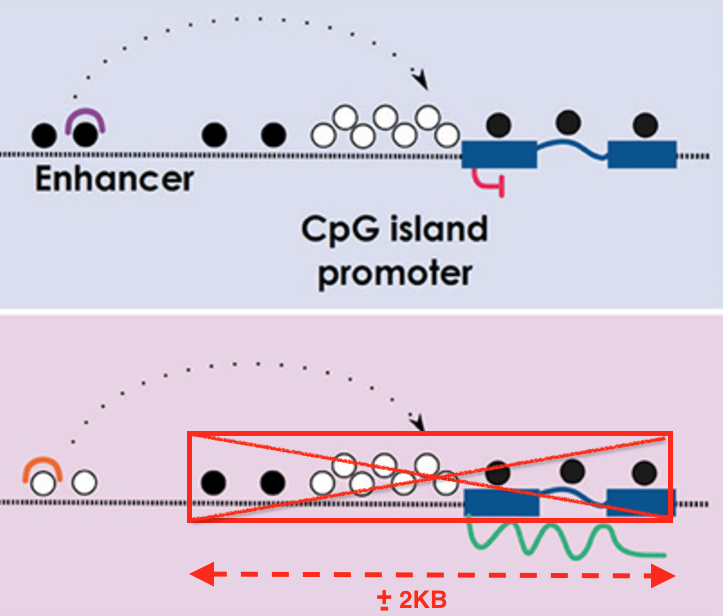
\includegraphics[width=0.7\linewidth]{step1.png}
 \end{figure}
\end{frame}


\begin{frame}{Step 2: Differentially methylated distal probes}
 \vspace*{-0.4cm}
 \begin{figure}
  \centering
  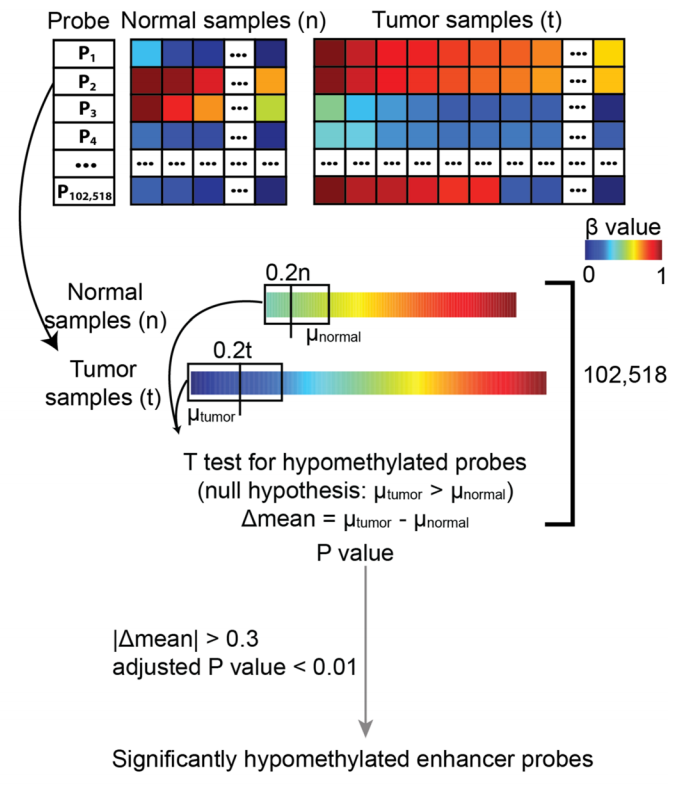
\includegraphics[width=0.57\linewidth]{ELMER/diffmeth.png}{\tiny{\\\vspace*{-0.2cm}Source: Yao et al. Genome Biology (2015)}}
 \end{figure}
\end{frame}



%\begin{frame}{Step 2: Differentially methylated distal probes}
% \begin{figure}
%  \centering
%  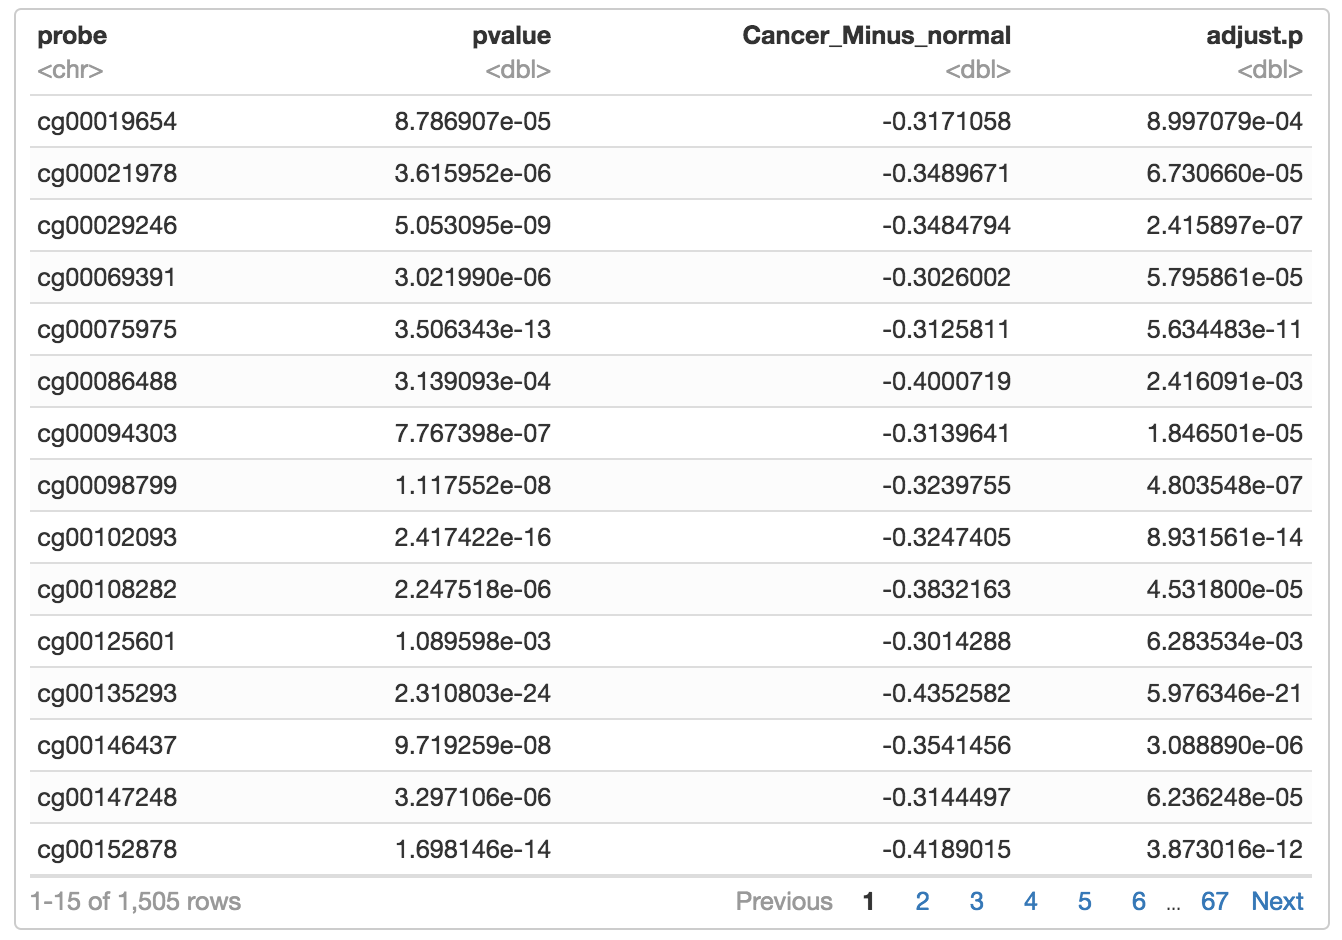
\includegraphics[width=0.9\linewidth]{ELMER/metdiff_tbl.png}
% \end{figure}
%\end{frame}

%\begin{frame}{Step 2: Differentially methylated distal probes}
% \begin{figure}
%  \centering
%  \includegraphics[width=1.0\linewidth]{ELMER/volcano_plot.pdf}
% \end{figure}
%\end{frame}

\begin{frame}{\normalsize{Groups $U$ and $M$ definition in \textit{(un)supervised} mode}} 

 \vspace*{-0.3cm}
 \begin{figure}
 \centering
  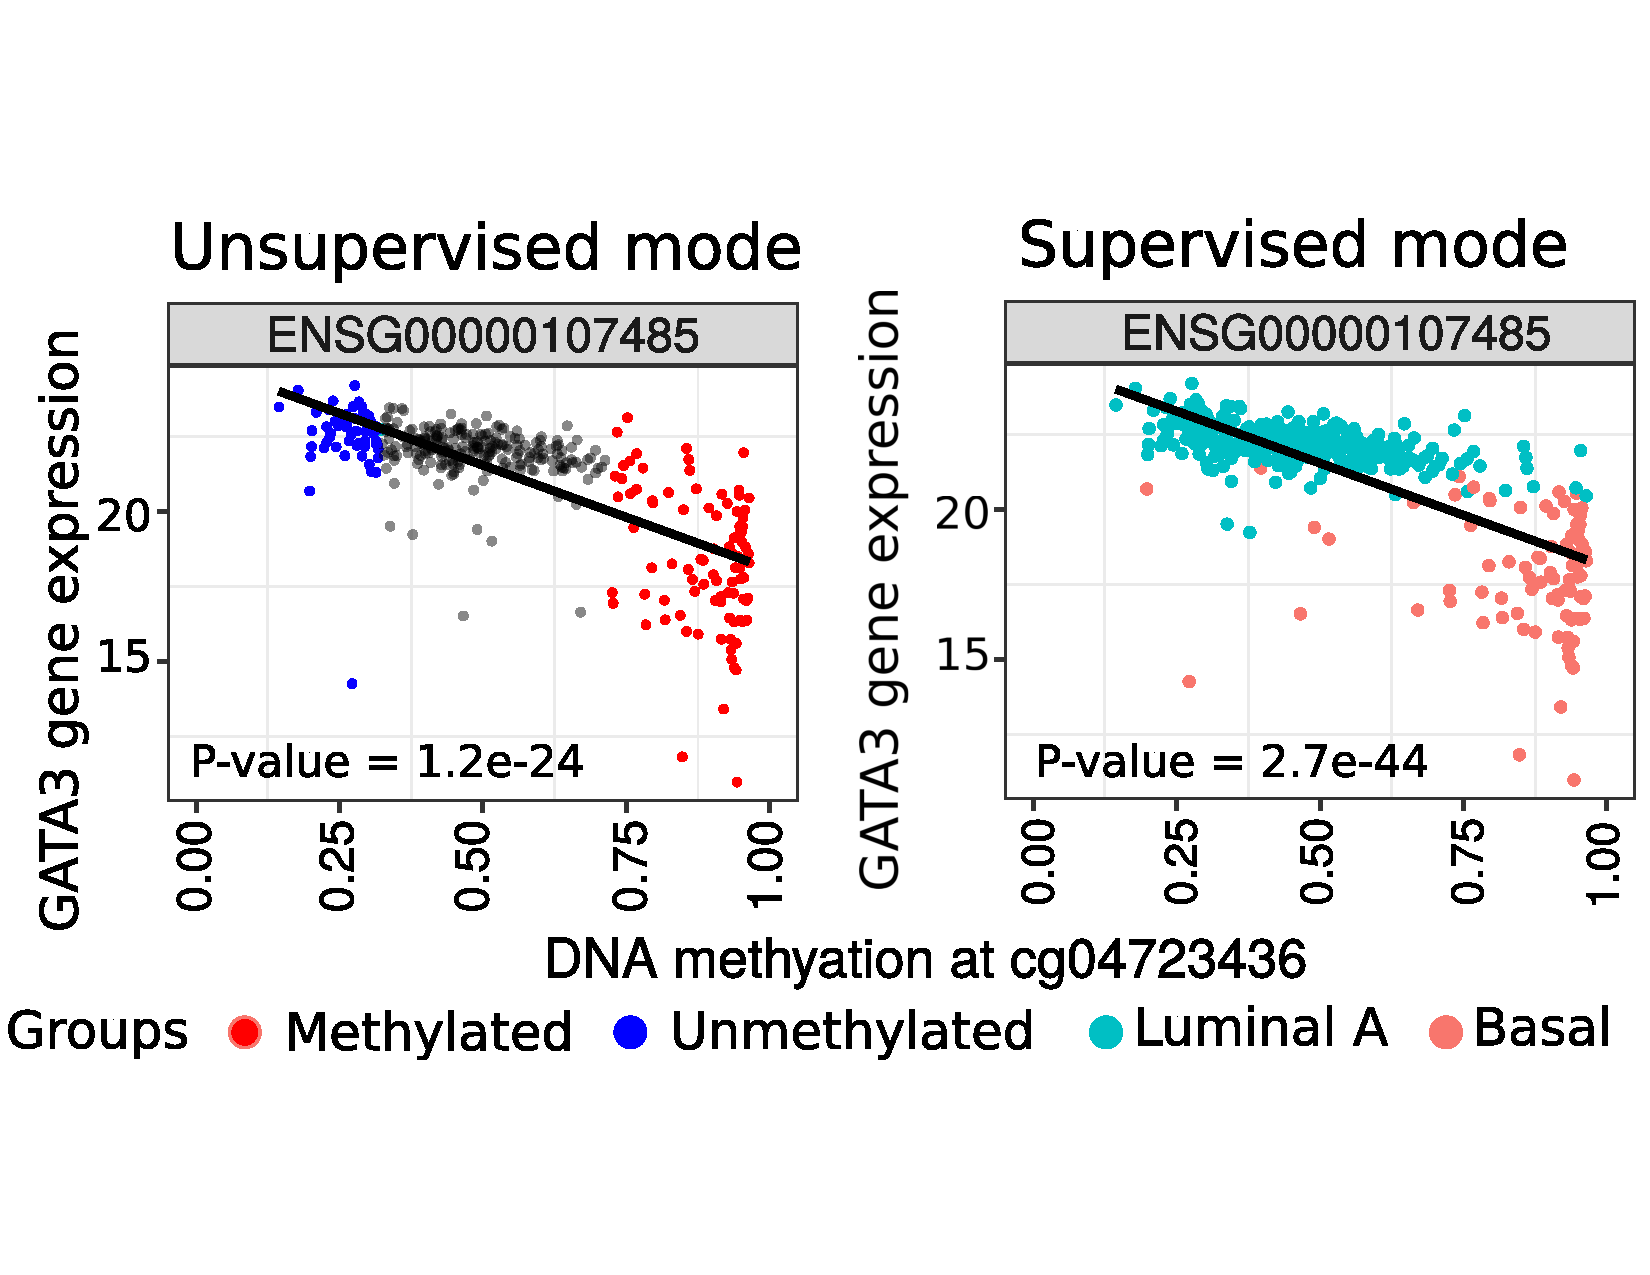
\includegraphics[width=1.0\linewidth]{ELMER/painel_mode.pdf}
  \scriptsize{\caption{ A:  \textit{unsupervised} mode; when minSubgroupFrac argument is set to 40\%, the methylated group is defined as the highest quintile and the unmethylated group as the lowest quintile; B:  \textit{supervised} mode; methylated and unmethylated group are defined as one of the known molecular subtypes.}}
 \end{figure}
\end{frame}


\begin{frame}{Step 3: Identification of putative target gene(s)}
 \vspace*{-0.4cm}
 \begin{figure}
\hspace*{-0.5cm}
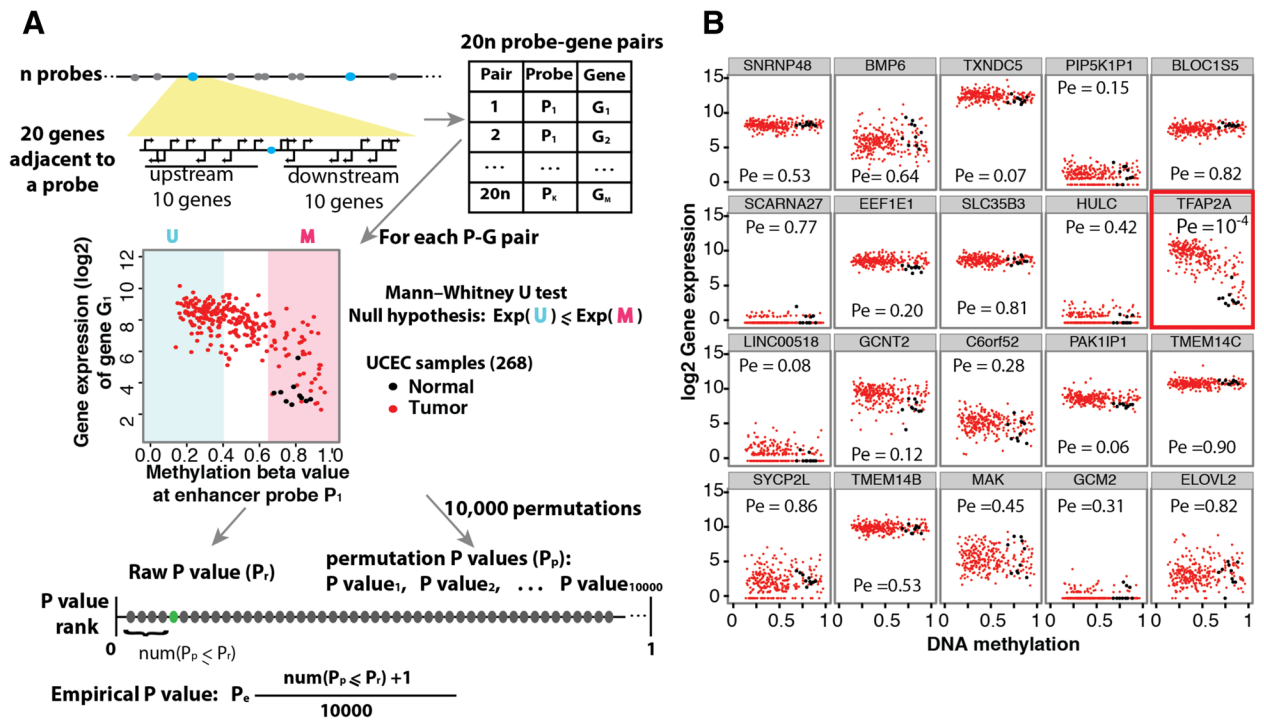
\includegraphics[width=1.1\linewidth]{ELMER/pair.png}{\tiny{\\\vspace{-0.3cm}Source: Yao et al. Genome Biology (2015)}}
 \end{figure}
\end{frame}



%\begin{frame}{Step 3: Probe-target gene pairs inferred}
% \begin{figure}
%  \centering
%  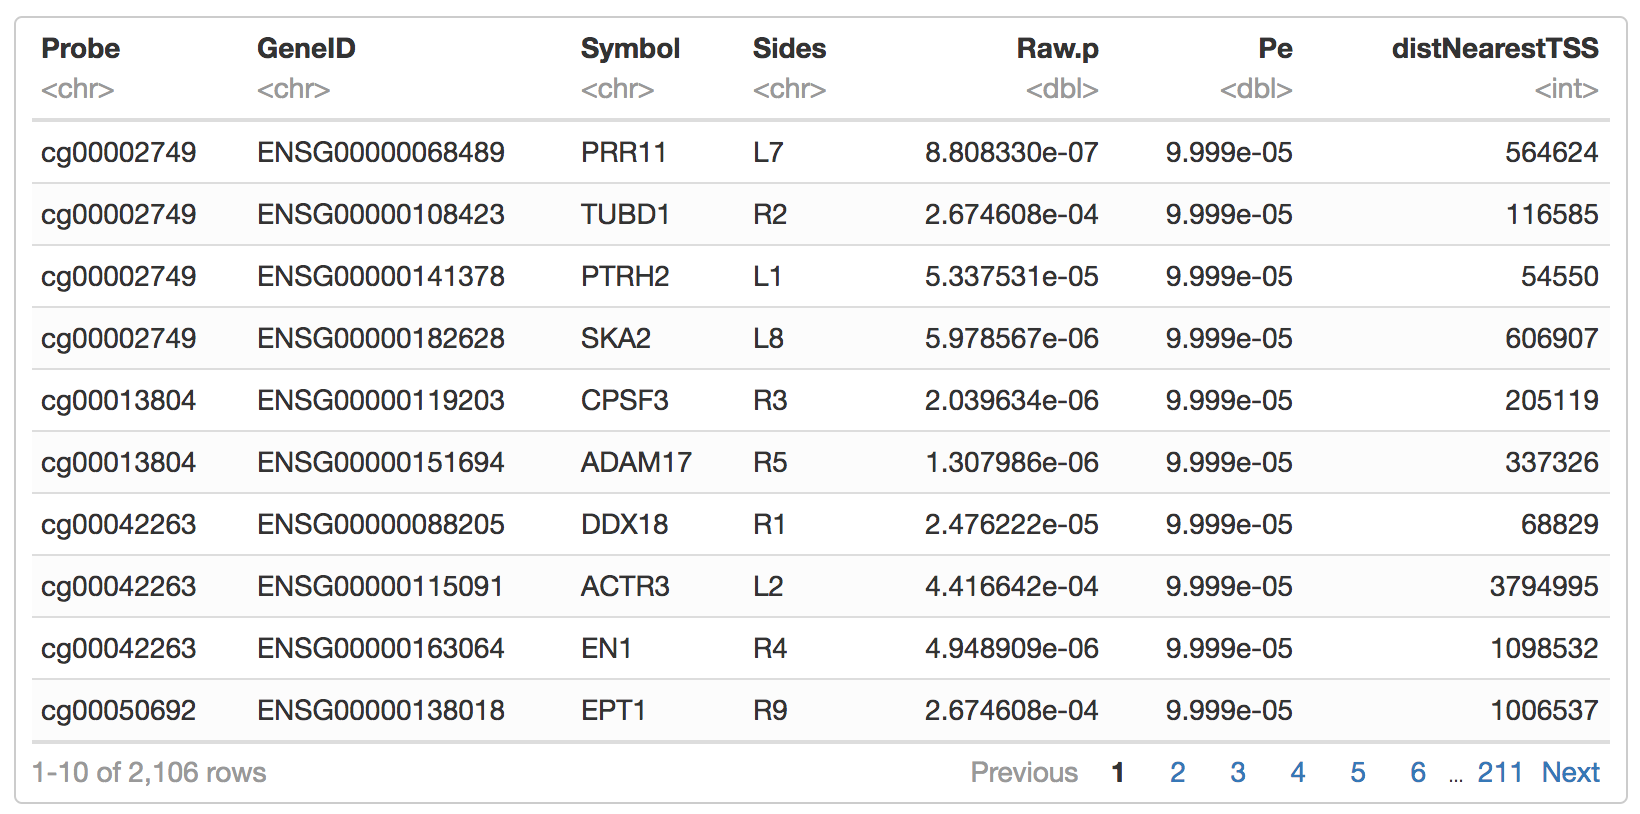
\includegraphics[width=1.0\linewidth]{ELMER/pairs_tbl.png}
% \end{figure}
%\end{frame}

\begin{frame}{Step 3: Probe-target gene pairs inferred}
 \vspace*{-0.3cm}
 \begin{figure}
  \centering
  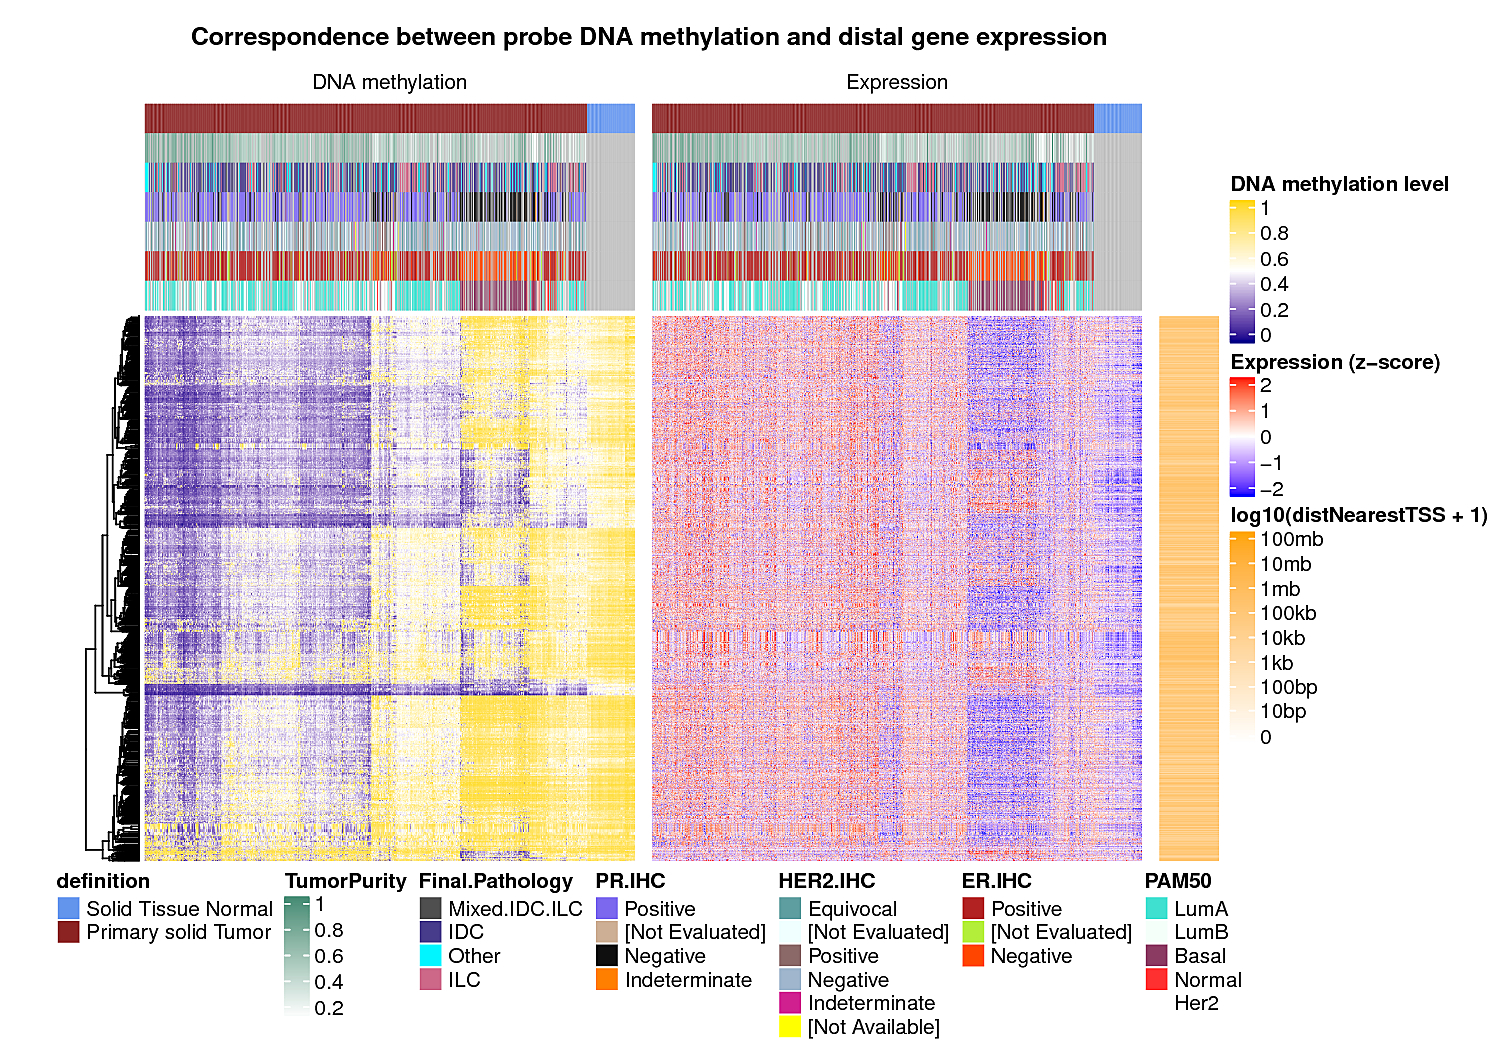
\includegraphics[width=1.0\linewidth]{ELMER/heatmappair.jpg}
 \end{figure}
\end{frame}

\begin{frame}{Chromatin state enrichment analysis}
 \vspace*{-0.4cm}
 \begin{figure}
  \centering
  \includegraphics[width=1.0\linewidth]{ELMER/painel_C.pdf} \end{figure}
\end{frame}


\begin{frame}{Step 4: Motif enrichment analysis}

 \vspace*{-0.3cm}
 \begin{figure}
  \centering
  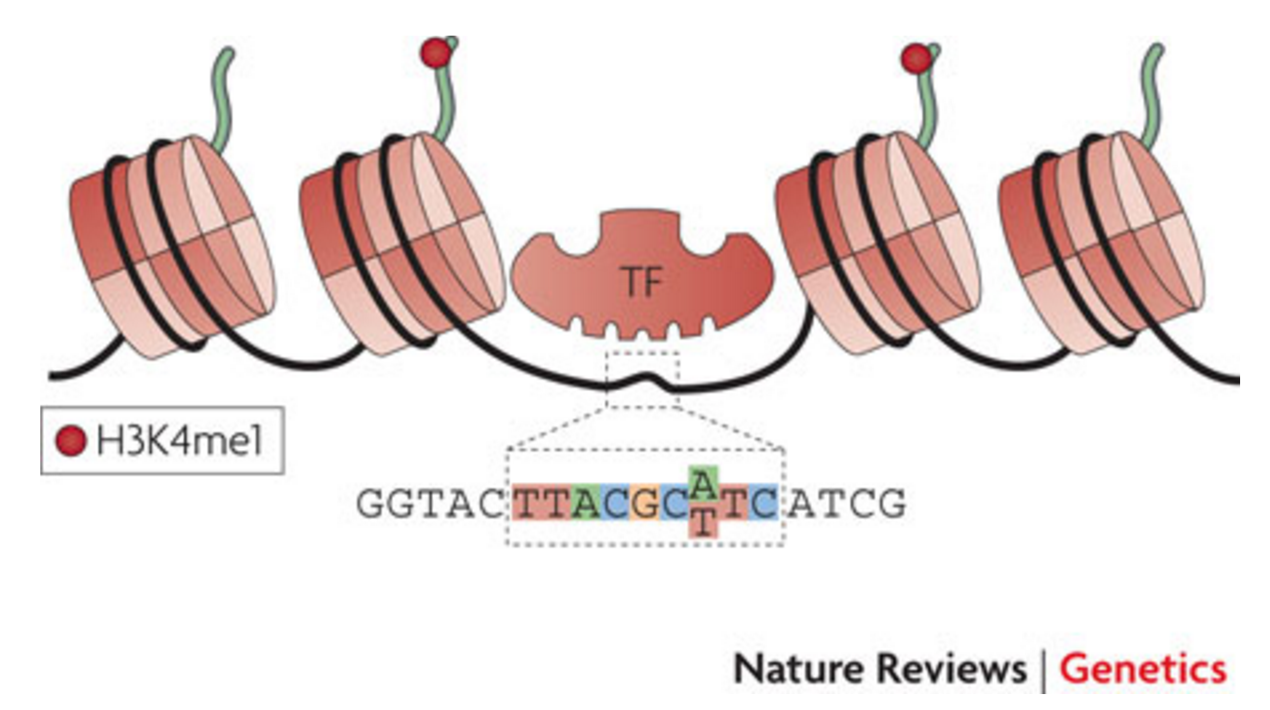
\includegraphics[width=1.0\linewidth]{ELMER/tf_binding.png}{\tiny{\\Hawkins RD, et al. Next-generation genomics: an integrative approach. Nature Reviews Genetics (2010)}}
 \end{figure}
\end{frame}


\begin{frame}{Step 4:  TF motifs source}
 \vspace*{-0.5cm}
 \begin{figure}
 \hspace*{-0.4cm}
  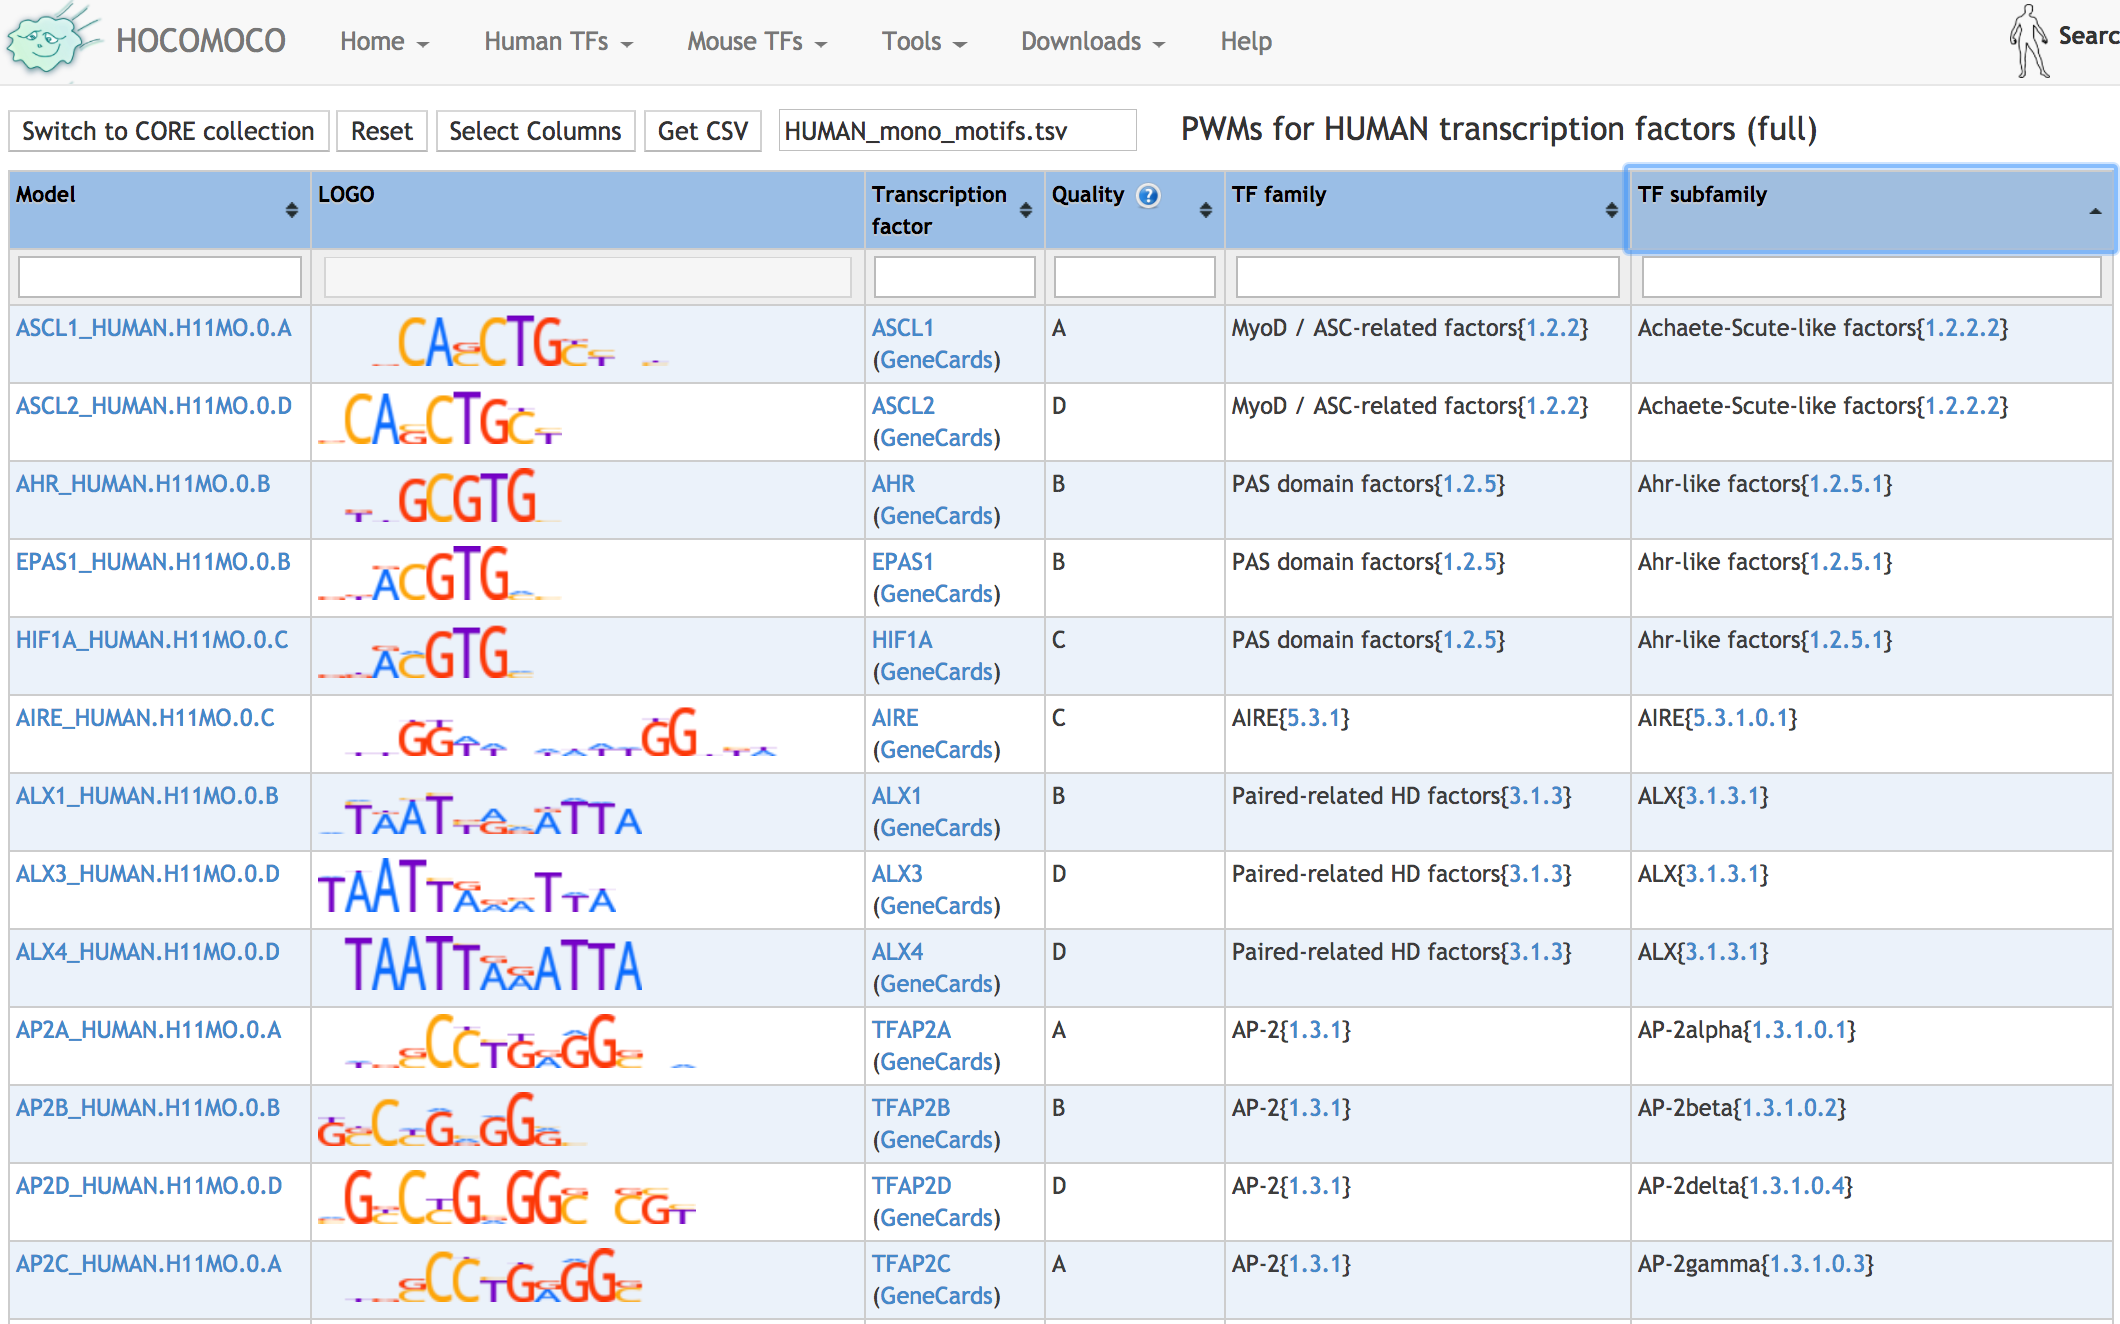
\includegraphics[width=1.1\linewidth]{ELMER/hocomoco.png}{\tiny{\\\vspace{-0.3cm}HOCOMOCO v11 (http://hocomoco11.autosome.ru/human/mono?full=true), Accessed: 25-12-2017}}
 \end{figure}
\end{frame}

\begin{frame}{Step 4: Motif enrichment analysis}

\begin{block}{Objective}
Evaluate the enrichment of transcription factors in certain genomic regions.
\begin{enumerate}
  \item Perform motif matching of transcription factors in probes regions (window $\pm250bp$). Performed using HOMER (Hypergeometric Optimization of Motif EnRichment) with HOCOMOCO motifs.
  \item Evaluate which transcription factors are more likely to occur in those regions than in background regions
  using Fisher'��s exact test with FDR correction.
\end{enumerate}
\end{block}
 \begin{exampleblock}{Fisher’s exact test}
 a: nb of input regions with a match for TF motif.\\
 b: nb of input regions with no match for TF motif.\\
 c: nb of background regions with a match for TF motif.\\
 d: nb of background regions with no match for TF motif.
 \end{exampleblock}

\end{frame}

\begin{frame}{Step 4: Motif enrichment analysis}
  \vspace{-0.2cm} 
  \begin{figure}
  \hspace*{-1cm} 
  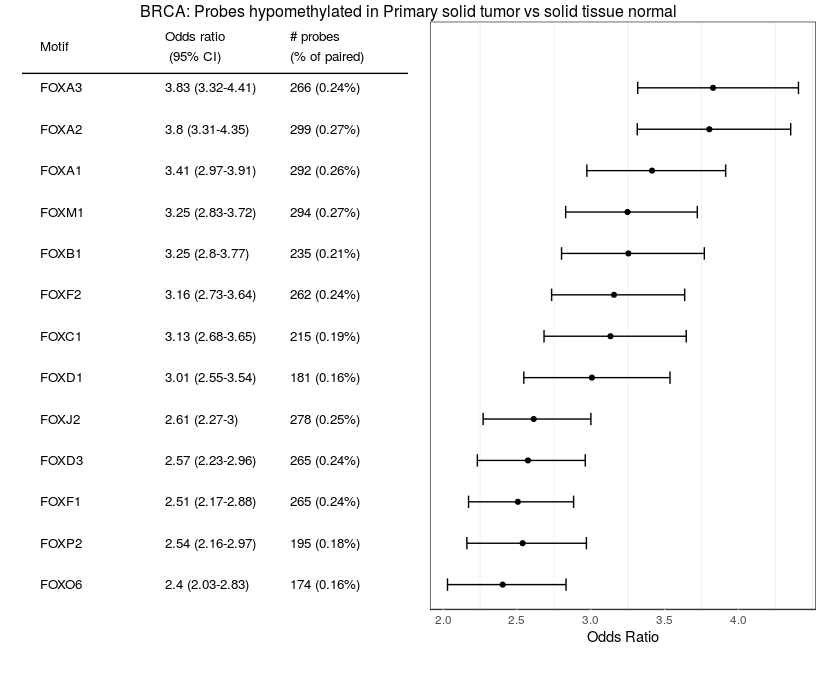
\includegraphics[width=0.9\linewidth]{ELMER/motif.png}
 \end{figure}
\end{frame}

%\begin{frame}{Step 4: Motif enrichment analysis}
% \begin{figure}
%  \centering
%  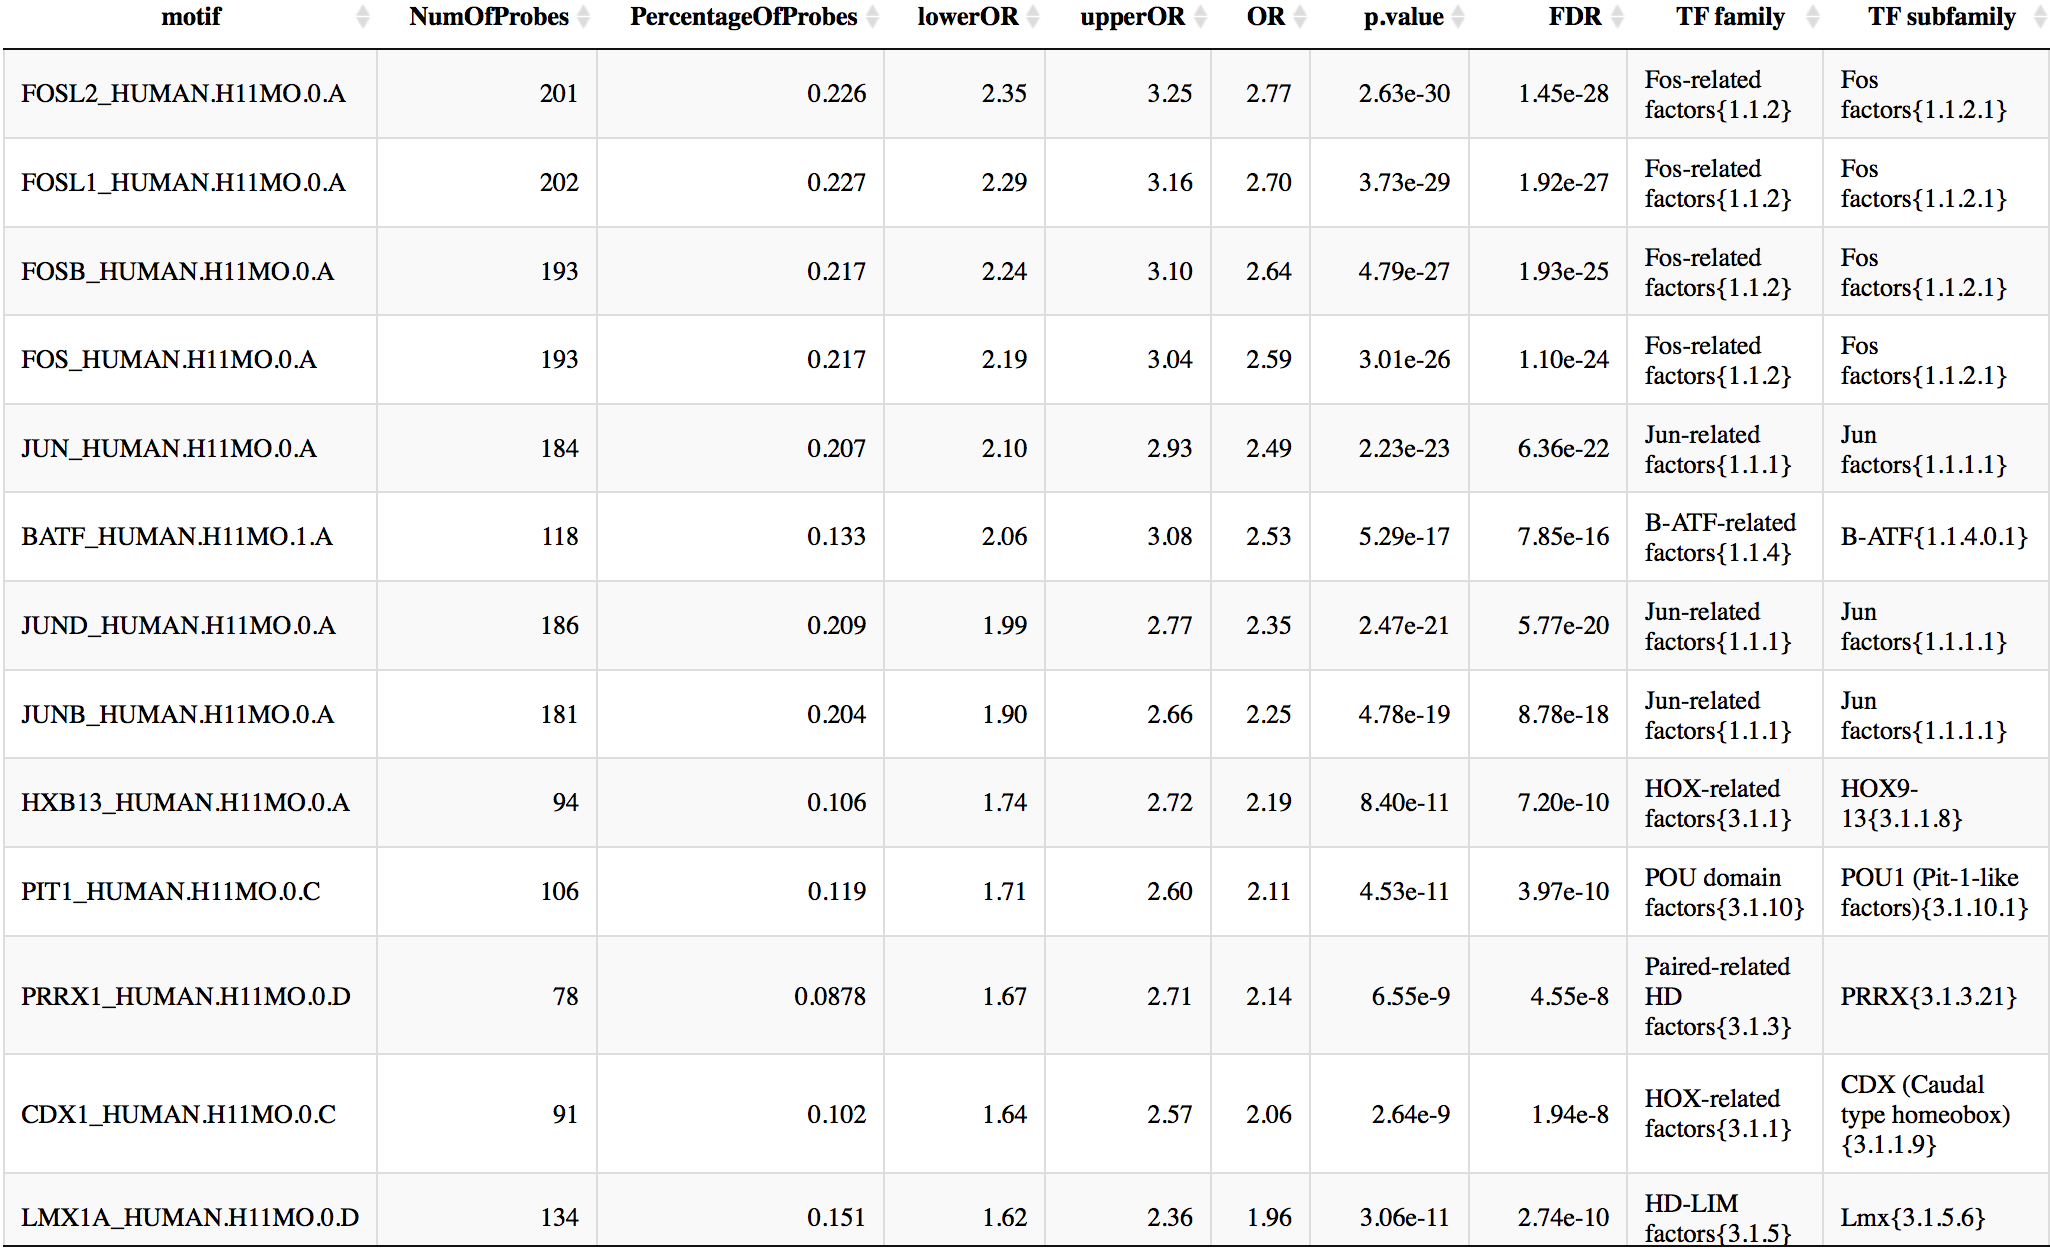
\includegraphics[width=1.0\linewidth]{ELMER/or_tbl.png}
% \end{figure}
%\end{frame}


%\begin{frame}{Step 5: Human TFs}
% \vspace*{-0.3cm}
% \begin{figure}
%  \centering
%  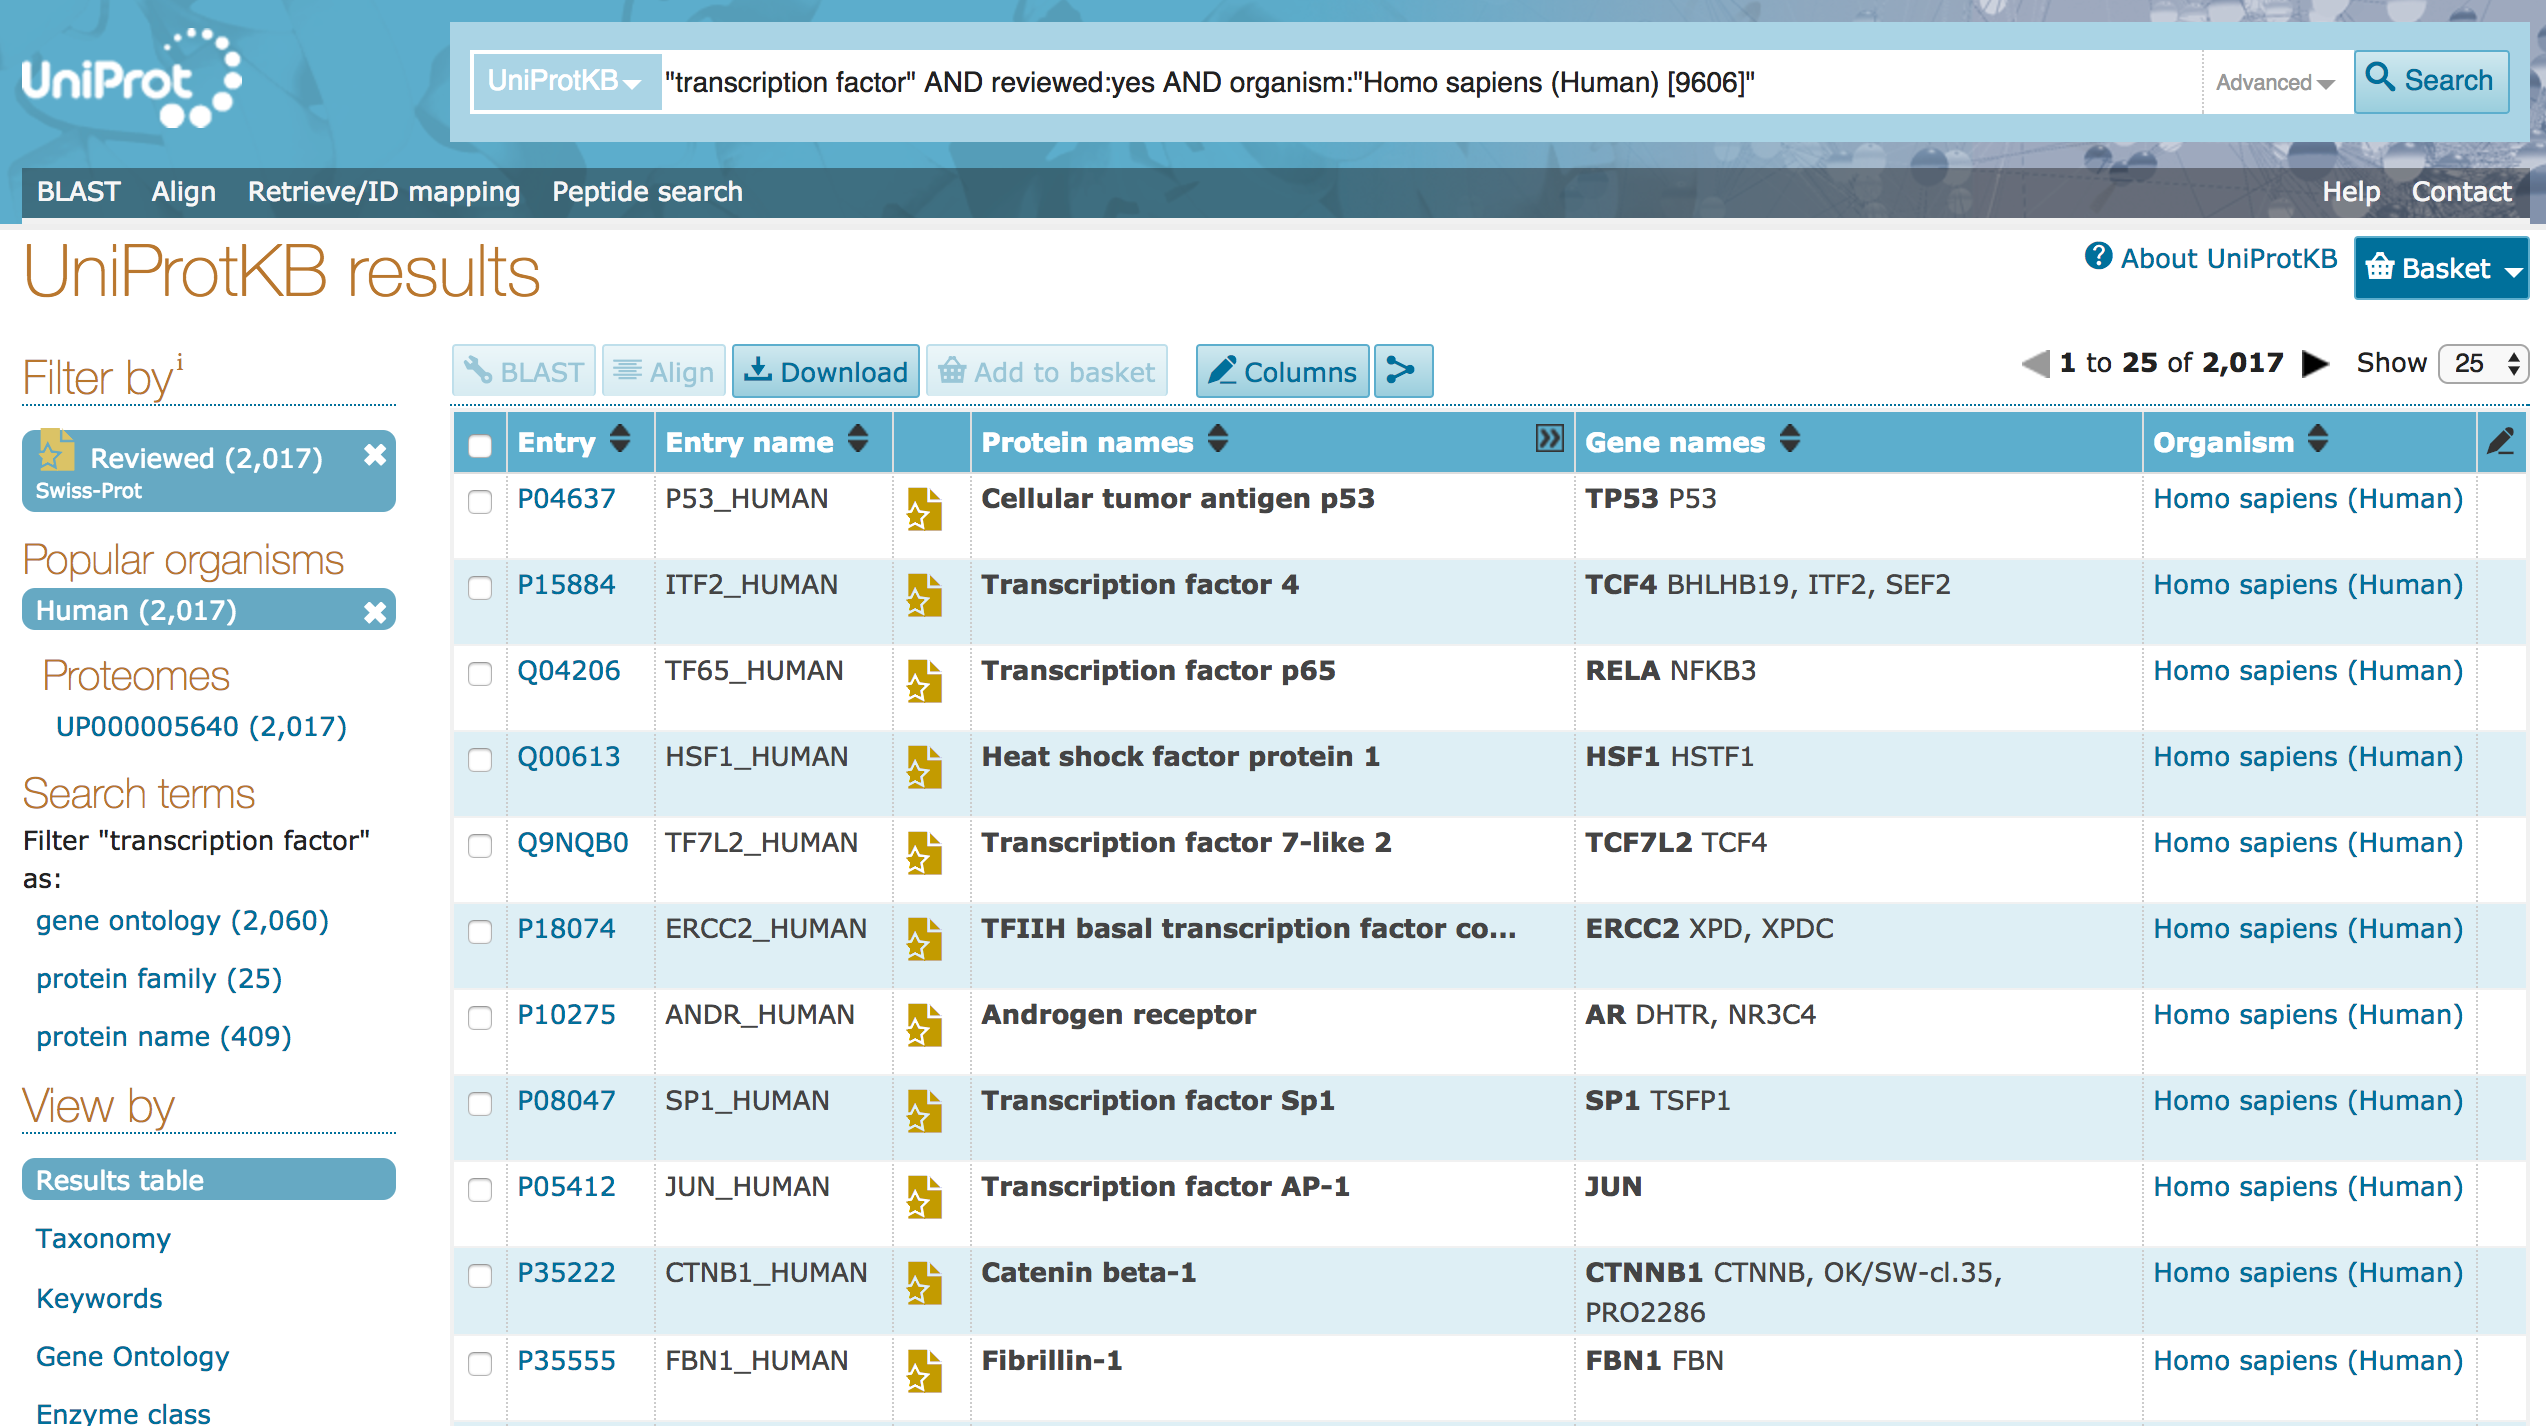
\includegraphics[width=1.0\linewidth]{ELMER/uniprot.png}
% \end{figure}
%\end{frame}

\begin{frame}{Step 5: Identification of master regulator TF}
\vspace*{-0.5cm}
 \begin{figure}
  \centering
  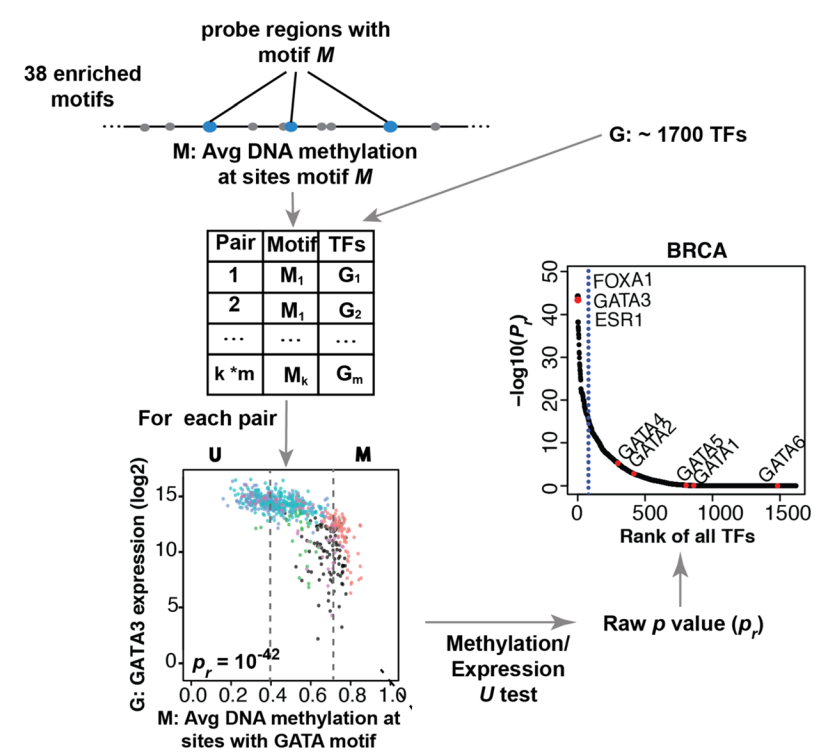
\includegraphics[width=0.75\linewidth]{ELMER/tfrank.png}{\tiny{\\ \vspace{-0.2cm}\href{https://genomebiology.biomedcentral.com/articles/10.1186/s13059-015-0668-3}{Source: Yao et al. Genome Biology (2015).}}}
 \end{figure}
\end{frame}


\begin{frame}{TFs ranking for the \textit{FOXA3} motif}
 \vspace*{-0.4cm}
 \begin{figure}
  \centering
  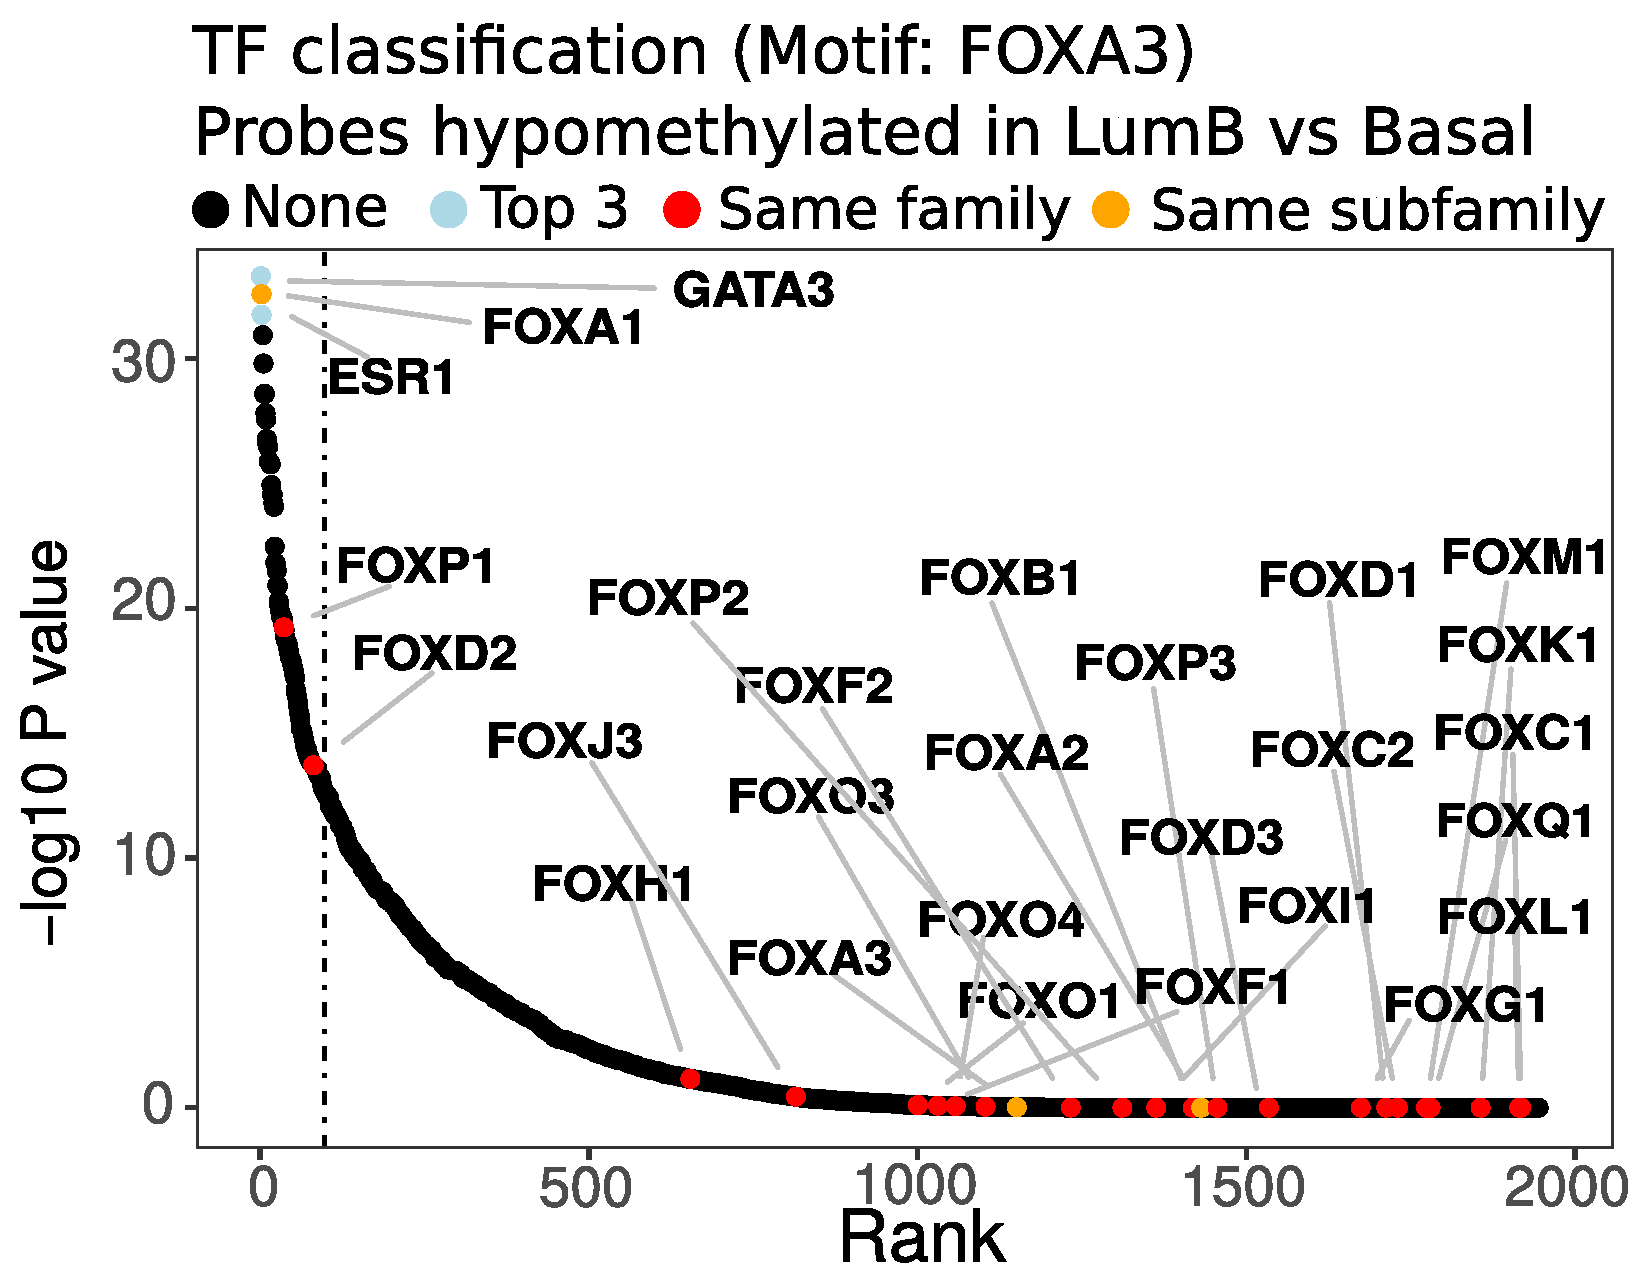
\includegraphics[width=0.9\linewidth]{ELMER/painel_D.pdf}
   \end{figure}
\end{frame}

%\begin{frame}{BRCA supervised analysis: Candidate MRs}
% \vspace*{-0.4cm}
% \begin{figure}
%  \centering
%  \includegraphics[width=0.48\linewidth]{ELMER/painel_E.pdf} \end{figure}
%\end{frame}



%\begin{frame}{Step 5: TF scatter plot}
% \begin{figure}
%  \centering
%  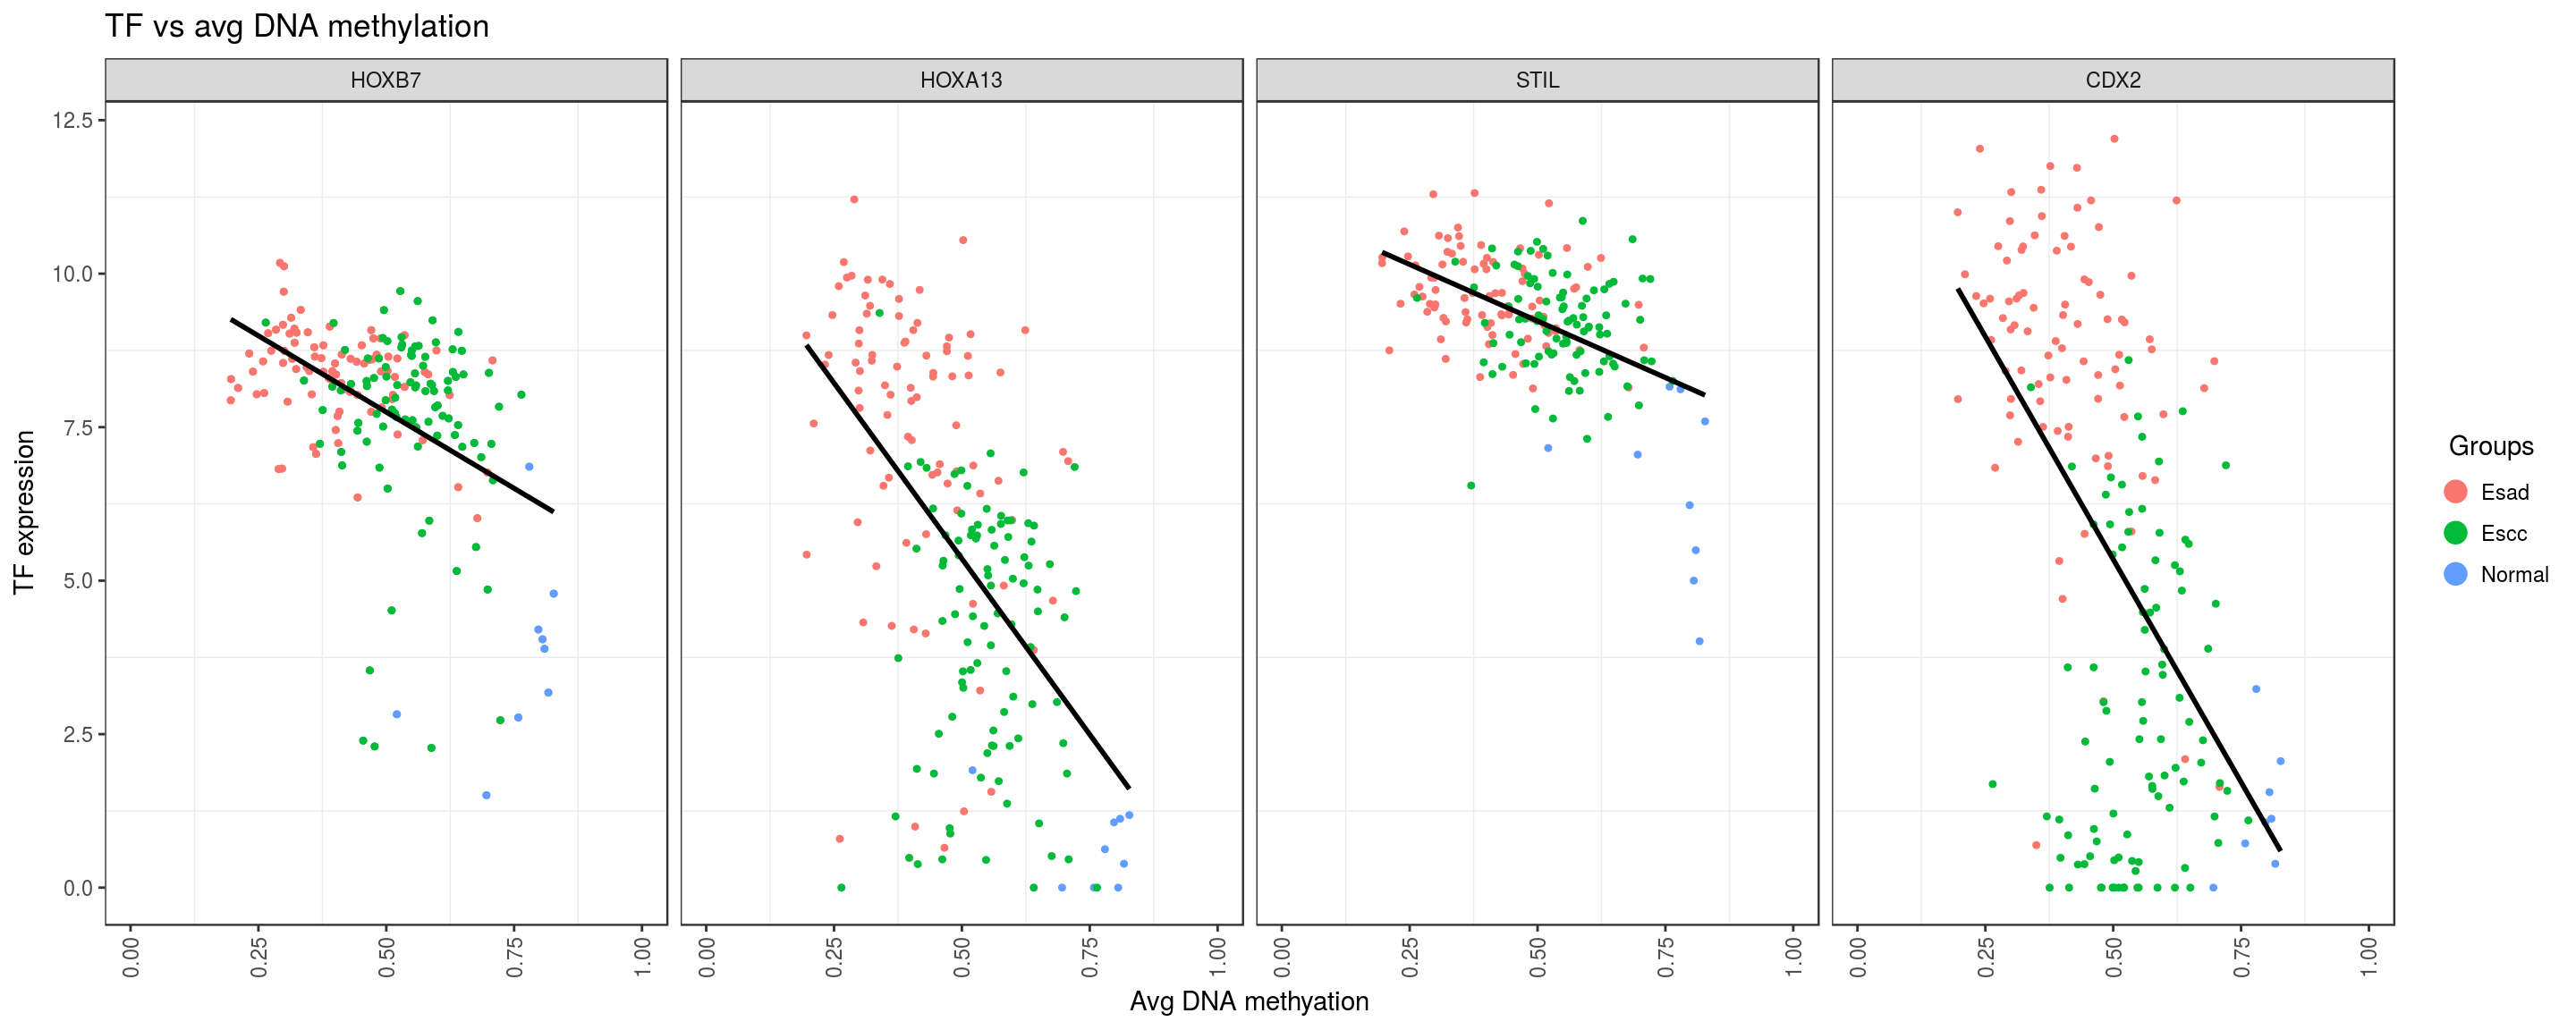
\includegraphics[width=1.0\linewidth]{ELMER/TF_plot_scatter.png}{\tiny{\\HOXB13 motif - Probes hypomethylated in esad vs normal}}
% \end{figure}
%\end{frame}

%\begin{frame}{Step 5: TF ranking plot}
% \vspace*{-0.5cm}
% \begin{figure}
%  \centering
  %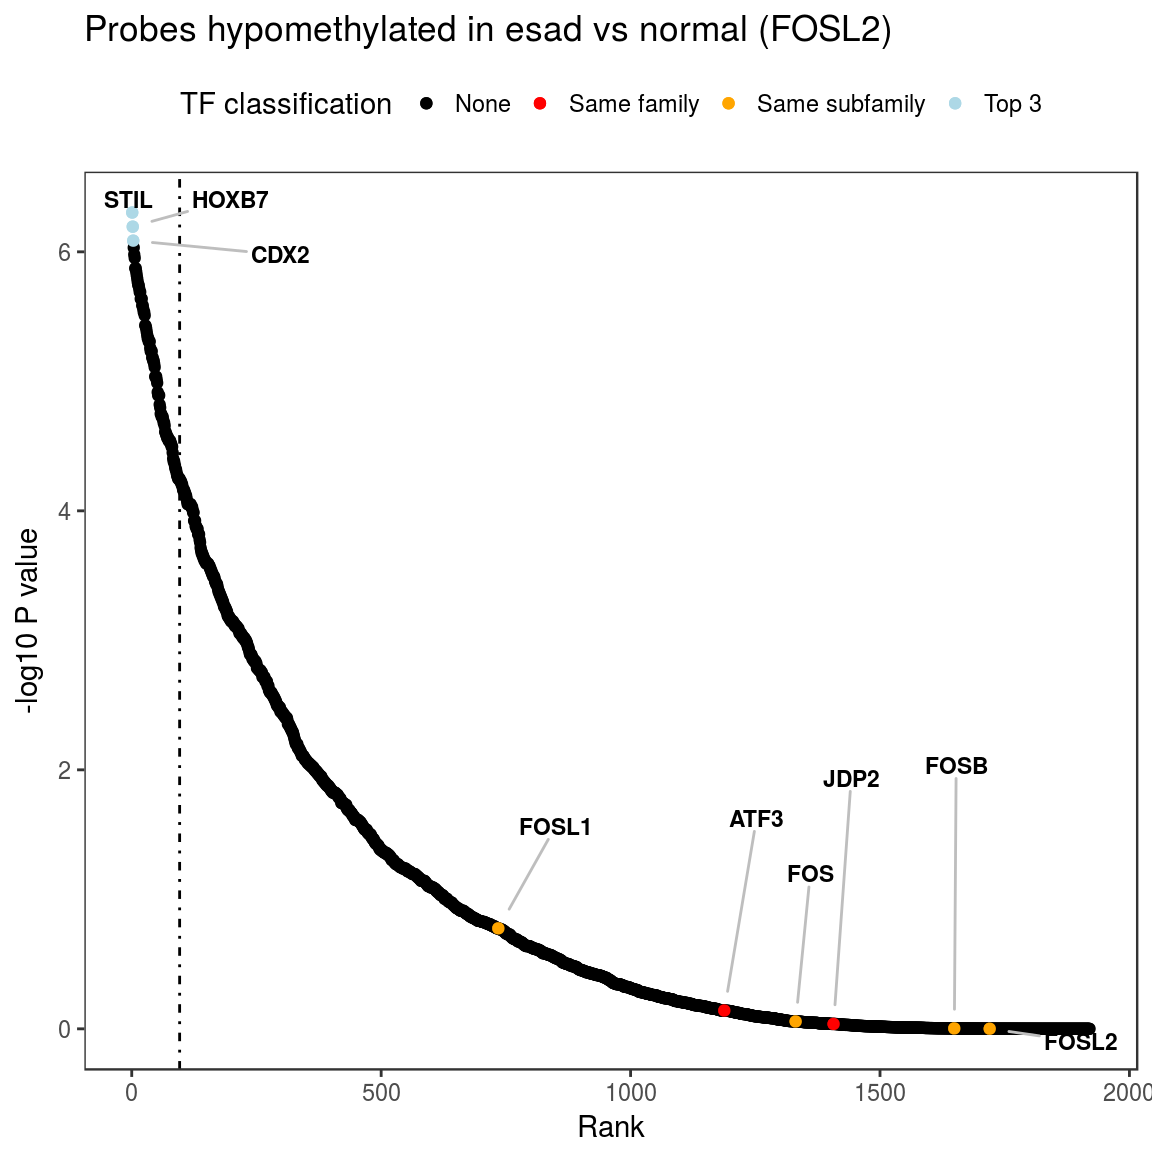
\includegraphics[width=0.45\linewidth]{ELMER/FOS_TF.png}
%  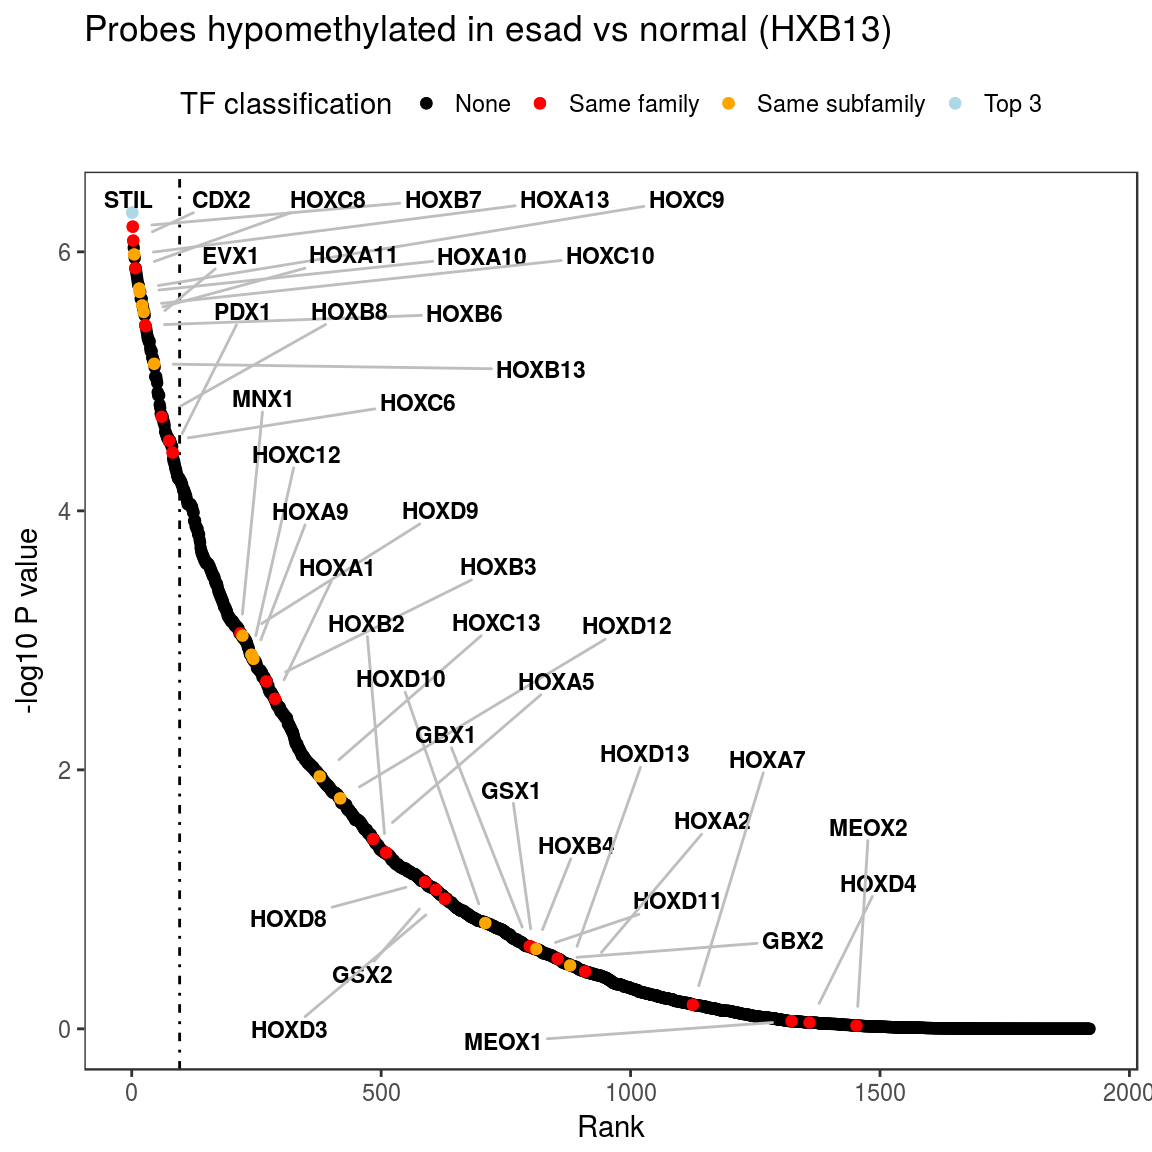
\includegraphics[width=0.7\linewidth]{ELMER/HOX_TF.png}
% \end{figure}
%\end{frame}

\begin{frame}{Step 5: Master Regulator TF table}
 \vspace{-0.5cm}
 \begin{figure}
  \hspace*{-0.5cm}
  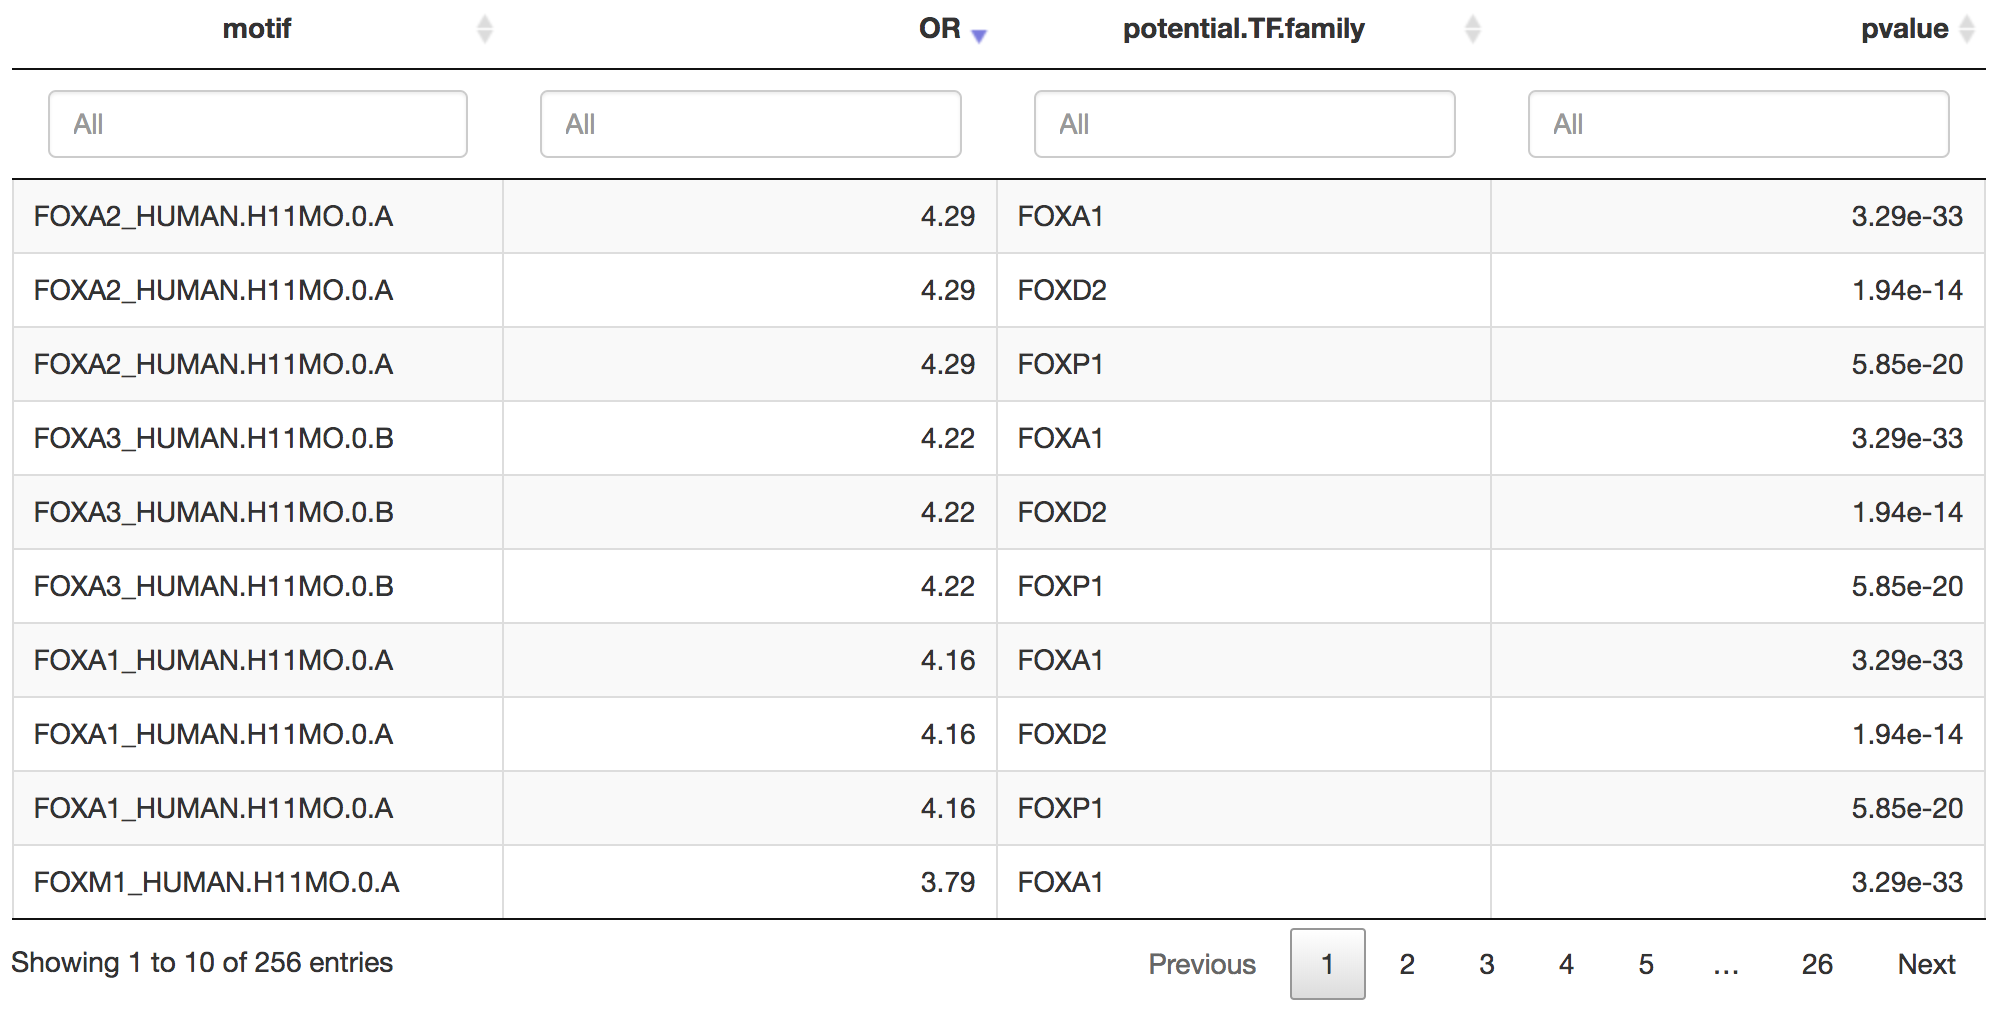
\includegraphics[width=1.1\linewidth]{ELMER/TF_tbl.png}
 \end{figure}
\end{frame}

\begin{frame}{ \normalsize{Main differences between ELMER old version (v.1) and the new version (v.2)}}
 \normalsize{
 \vspace{-0.5cm}
\begin{table}
\centering
\label{tab:summary}
%{\def\arraystretch{2}\tabcolsep=10pt
\resizebox{\textwidth}{!}{%
\begin{tabular}{@{}m{4cm}m{6cm}m{7cm}@{}}
\toprule
\toprule
\multicolumn{1}{c}{\textbf{Features}} & \multicolumn{1}{c}{\textbf{ELMER Version 1}} & \multicolumn{1}{c}{\textbf{ELMER Version 2}}   \\ \midrule \midrule
Primary data structure      & mee object (custom data structure)   & MAE object (Bioconductor data structure) \\ \midrule
Auxiliary data      & Manually created   & Programmatically created \\\midrule
Number of human TFs       & 1,982 & 2,014 (UniProt database)    \\\midrule
Number of TF motifs      & 91    & 771  (HOCOMOCO v11 database)    \\\midrule
TF classification &  78 families         & 82 families and 331 subfamilies \newline(TFClass database, HOCOMOCO) \\\midrule
Analysis performed            & Normal vs tumor samples & Group 1 vs group 2   \\ \midrule
Statistical grouping            & Unsupervised only & Unsupervised or supervised using labeled groups   \\ \midrule
TCGA data source      & The Cancer Genome Atlas (TCGA)    & The NCI's Genomic Data Commons (GDC)     \\\midrule
Genome of reference      & GRCh37 (hg19)      & GRCh37 (hg19)/GRCh38 (hg38)          \\\midrule
DNA methylation platforms             & HM450  & EPIC and HM450            \\\midrule
Graphical User Interface (GUI)        & None  & TCGAbiolinksGUI     \\\midrule
Automatic report        & None  & HTML summarizing results    \\\midrule
Annotations      & None  & StateHub   \\
\bottomrule
\end{tabular}
}
%}
\end{table}
 }
\end{frame}



\section{Case of study}

\begin{frame}{Case study: TCGA Breast Invasive Carcinoma (BRCA)}
 \begin{table}[ht!]
  \centering
  \caption{Summary of the available samples in TCGA for BRCA}
  \scriptsize

  \begin{tabular}{p{2.3cm}p{2.4cm}p{2.4cm}p{1cm}}
   \toprule
   Group               & Samples w/ DNA methylation (450K) & Samples w/ gene expression (FPKM-UQ) & Samples w/ both \\ \midrule
   Primary solid Tumor & 791                               & 1102                                 & 778             \\
   Solid Tissue Normal & 96                                & 113                                  & 83              \\
   \bottomrule
  \end{tabular}
 \end{table}

 %\begin{table}[ht!]
 % \centering
 % \caption{Results supervised mode}
 % \scriptsize

 % \begin{tabular}{p{2.8cm}p{2.4cm}}
 %  \toprule
 %  Inferred gene-probe pairs & 2167 \\
 %  Enriched motifs           & 312  \\
 %  Master Regulator TF      & 17   \\
 %  \bottomrule
 % \end{tabular}
 %\end{table}
 
 \begin{table}[h!]
\centering
\caption{Number of samples of the molecular subtypes of breast cancer}
\scriptsize
\begin{tabular}{|c|c|}
\hline
\textbf{Molecular subtype} & \textbf{Number of samples} \\ \hline
Basal & 85  \\ \hline
Her2 & 34 \\  \hline
LumA & 288 \\  \hline
LumB & 117 \\  \hline
Normal-like & 22 \\ \hline
\end{tabular}
\end{table}

 
\end{frame}


%\begin{frame}{Step 3: Probe-target gene pairs inferred}
%\vspace*{-0.5cm}
%\begin{figure}
% \centering
%   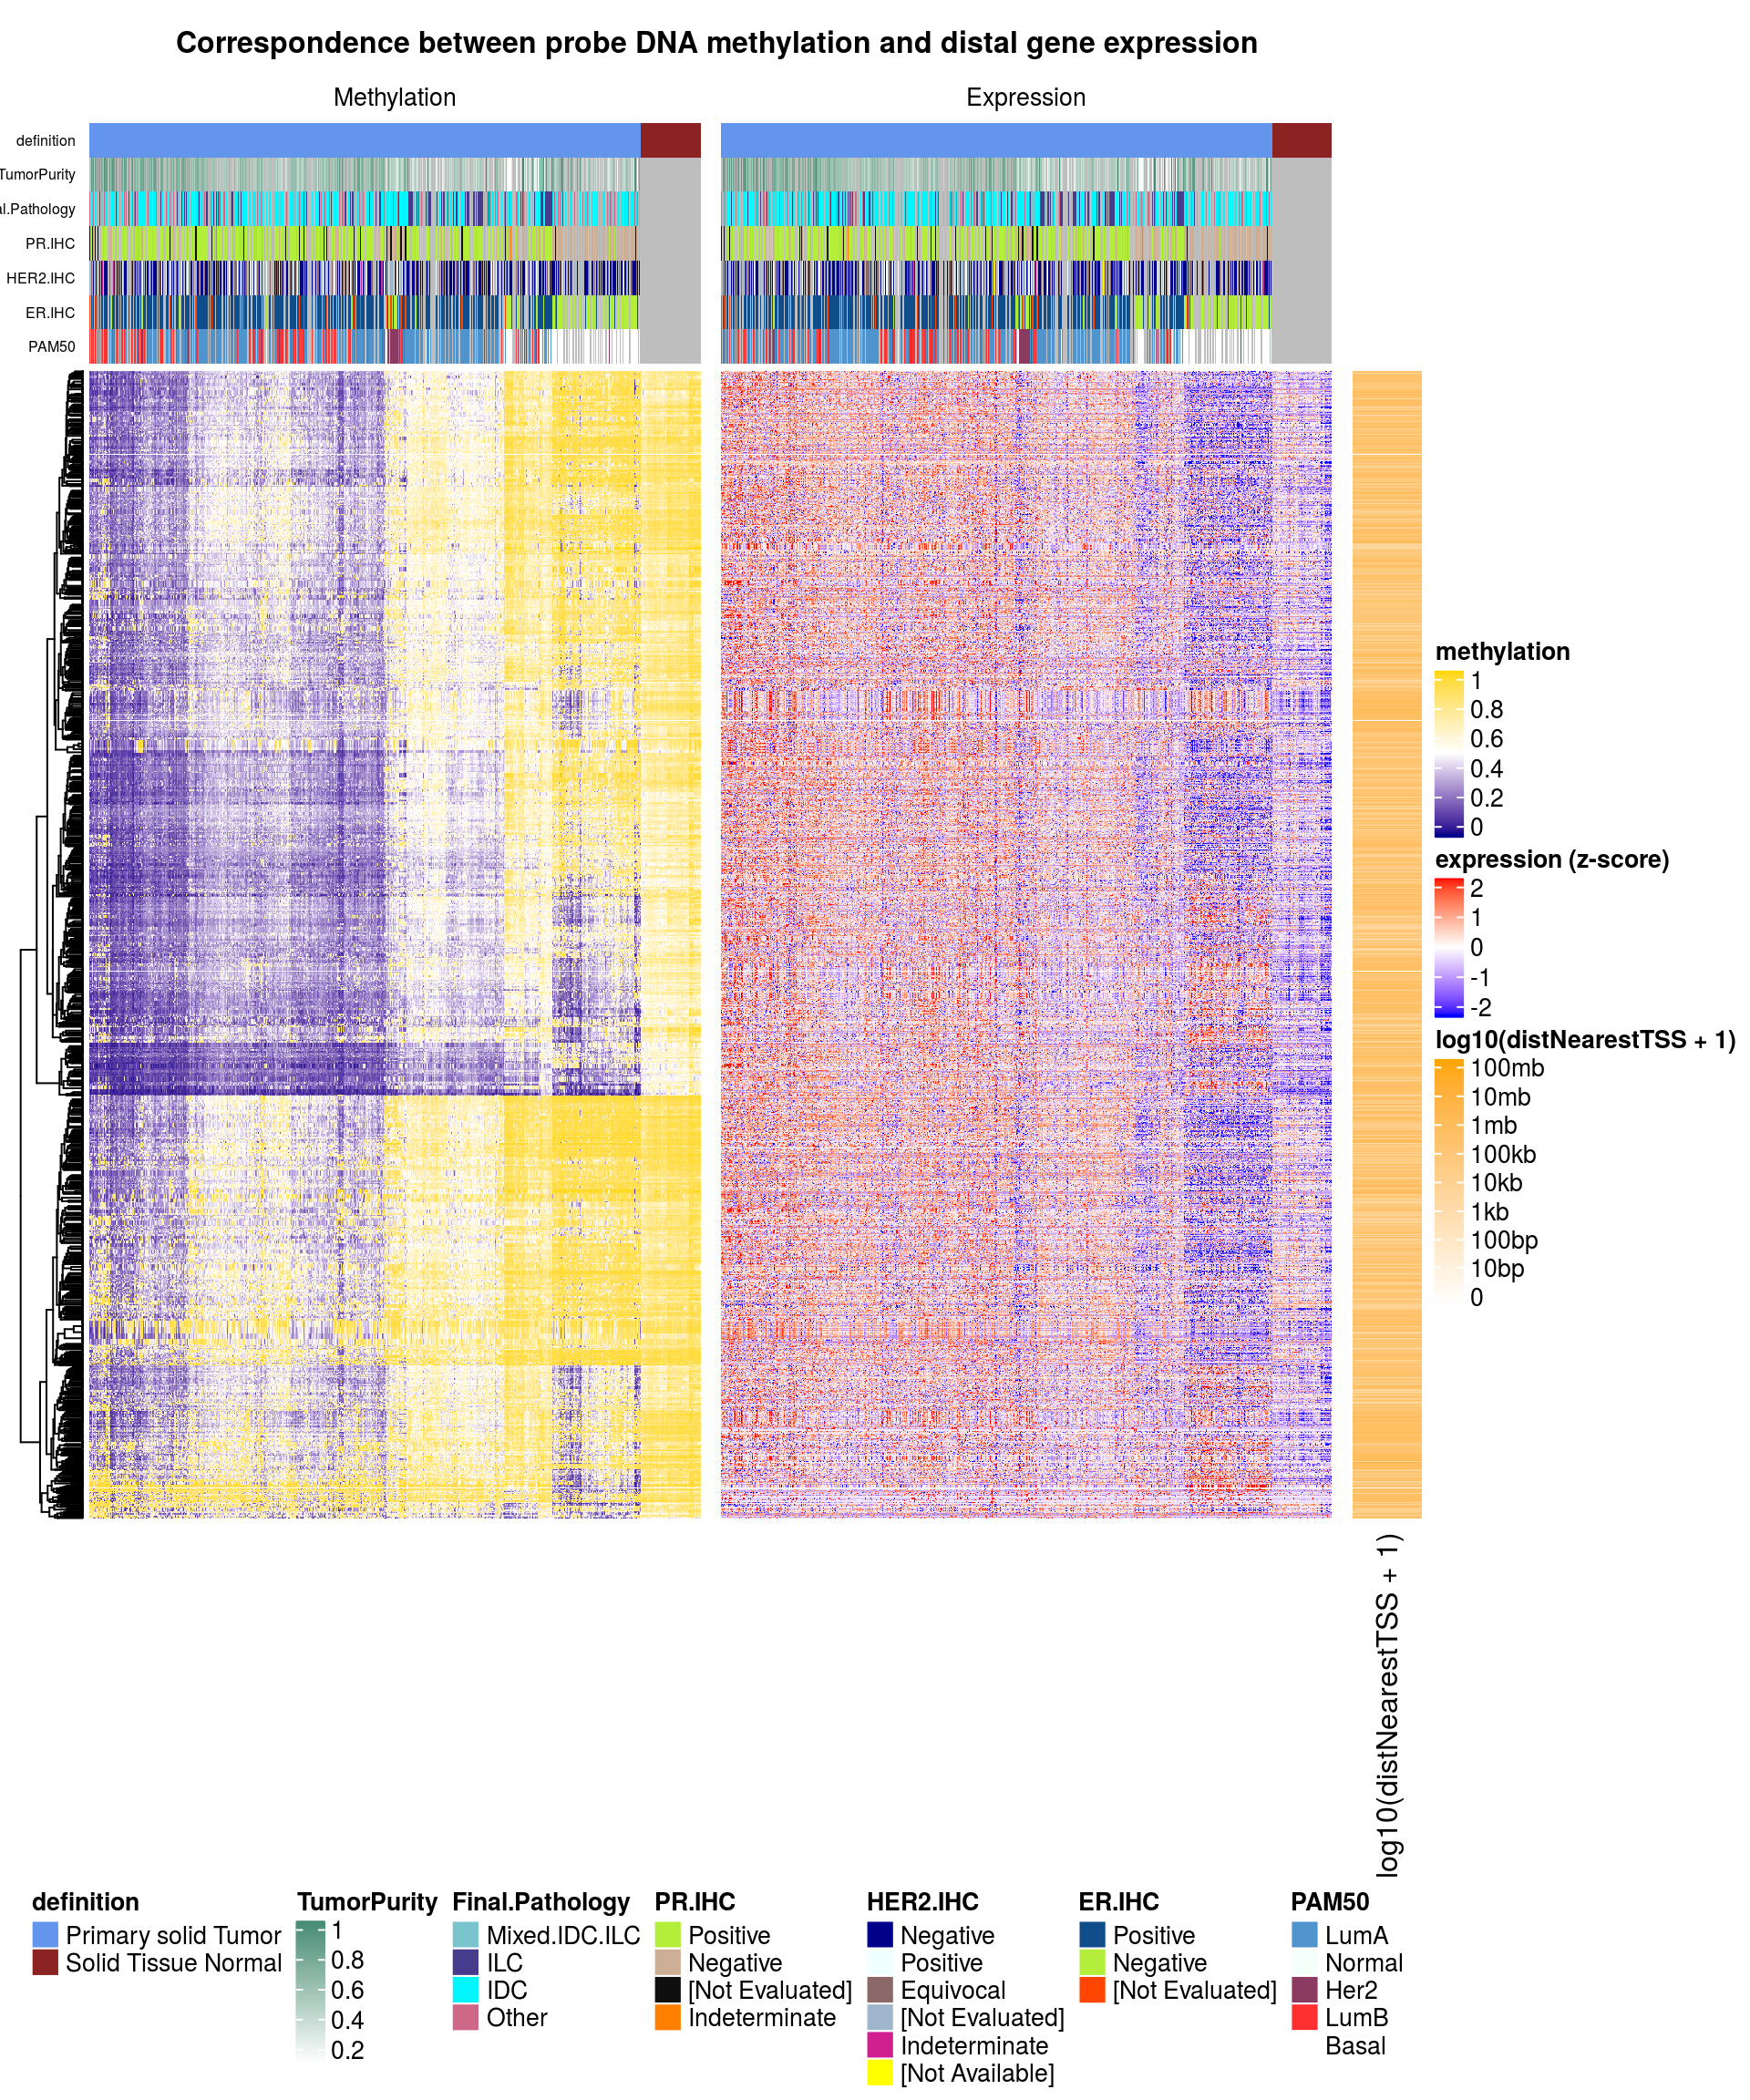
\includegraphics[width=0.75\linewidth]{ELMER/BRCA_heatmap.png}
%   \end{figure}
%\end{frame}


%\begin{frame}{Top enriched motifs}
% \vspace*{-0.3cm}
% \begin{figure}
%  \centering
%  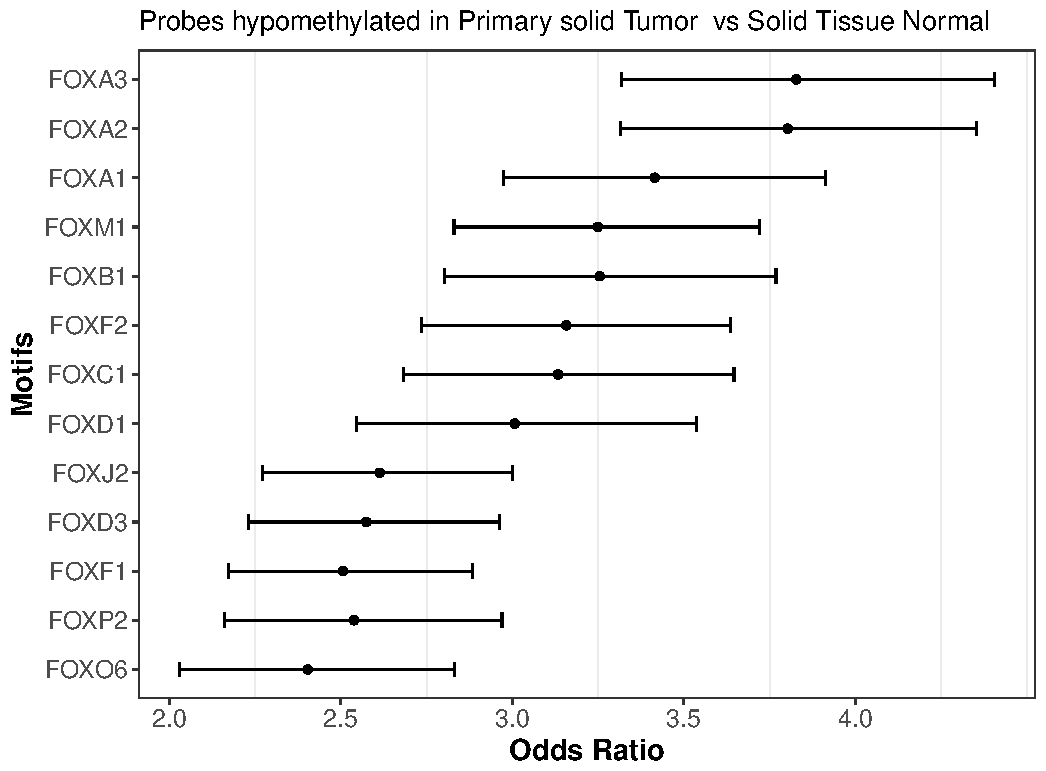
\includegraphics[width=0.9\linewidth]{ELMER/motif_new.pdf}
% \end{figure}
%\end{frame}


%\begin{frame}{TF ranking plot - FOXA3 motif}
% \vspace*{-0.3cm}
% \begin{figure}
%  \centering
%  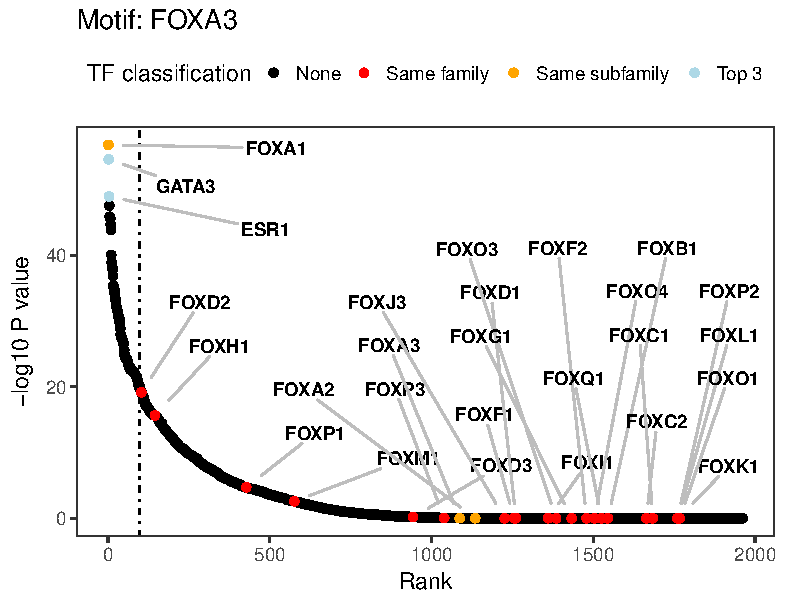
\includegraphics[width=0.9\linewidth]{ELMER/TF_raking.pdf}
% \end{figure}
%\end{frame}

%\begin{frame}{DNA methylation at motifs vs TF expression}
% \begin{figure}
%  \centering
%  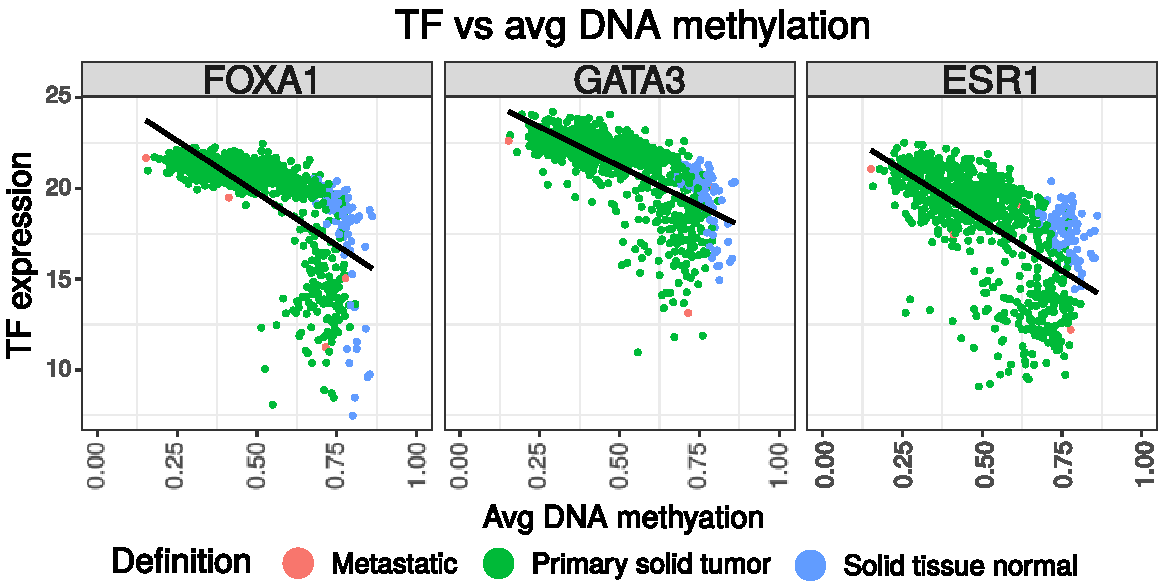
\includegraphics[width=1.0\linewidth]{ELMER/BRCA_TF_scatter.pdf}
% \end{figure}
%\end{frame}


%\begin{frame}{Candidate master regulator TF}
% \vspace*{-0.3cm}
% \begin{figure}
%  \centering
%  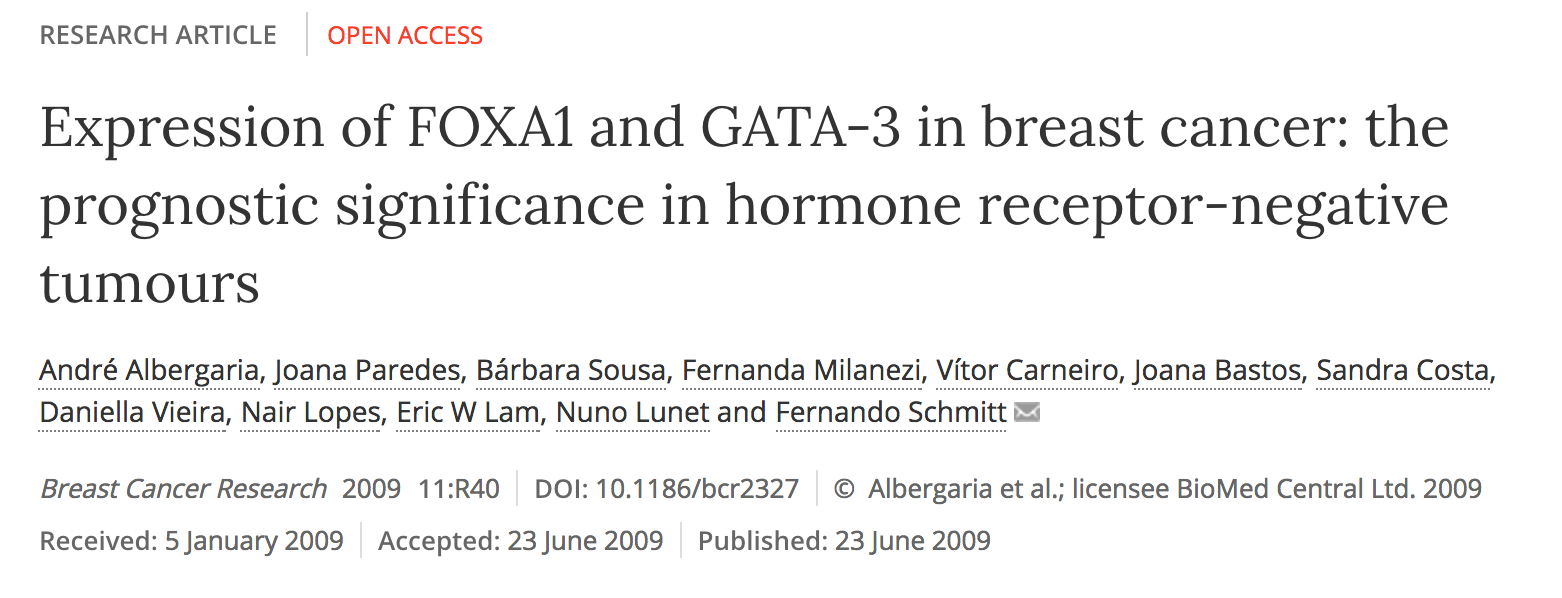
\includegraphics[width=0.8\linewidth]{ELMER/paper4.png}\\
 % 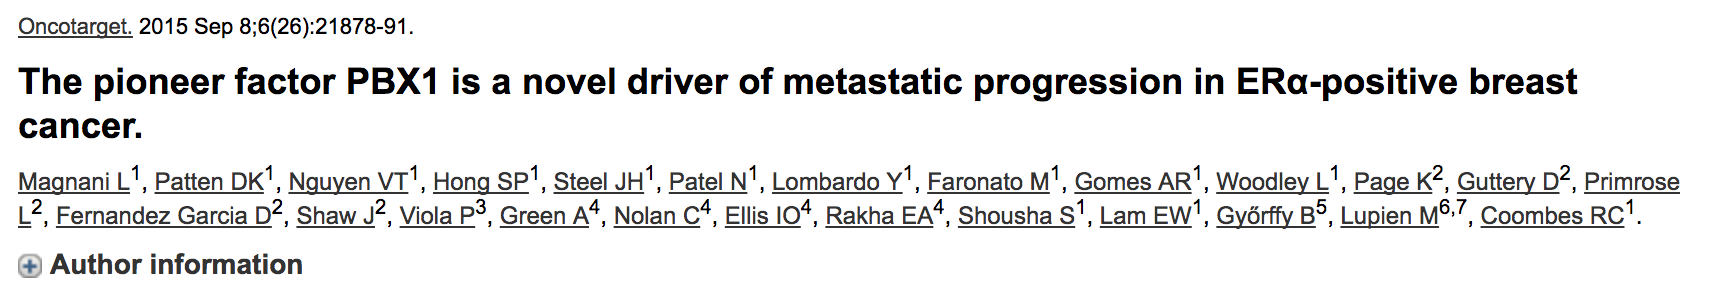
\includegraphics[width=0.8\linewidth]{ELMER/paper1.png}\\
%  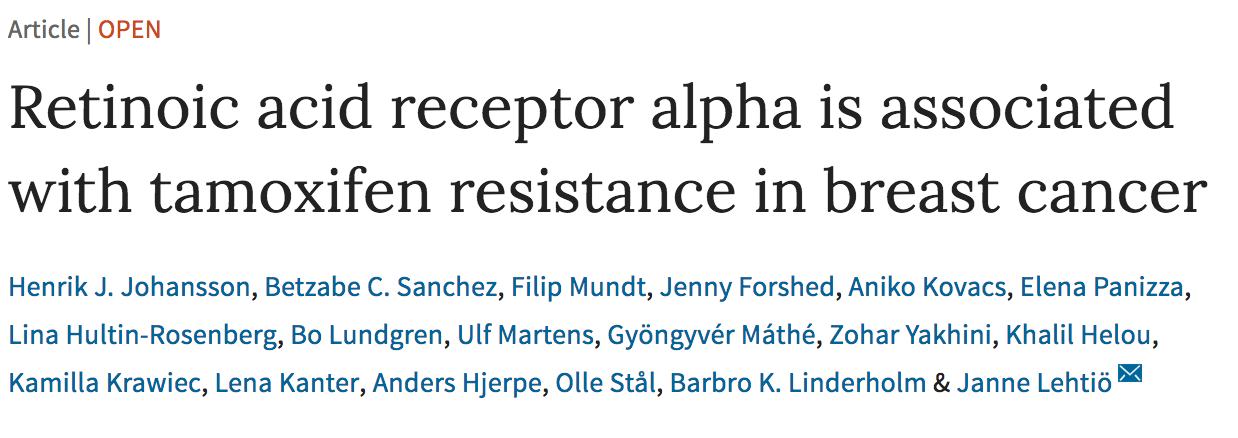
\includegraphics[width=0.8\linewidth]{ELMER/paper2.png}
  %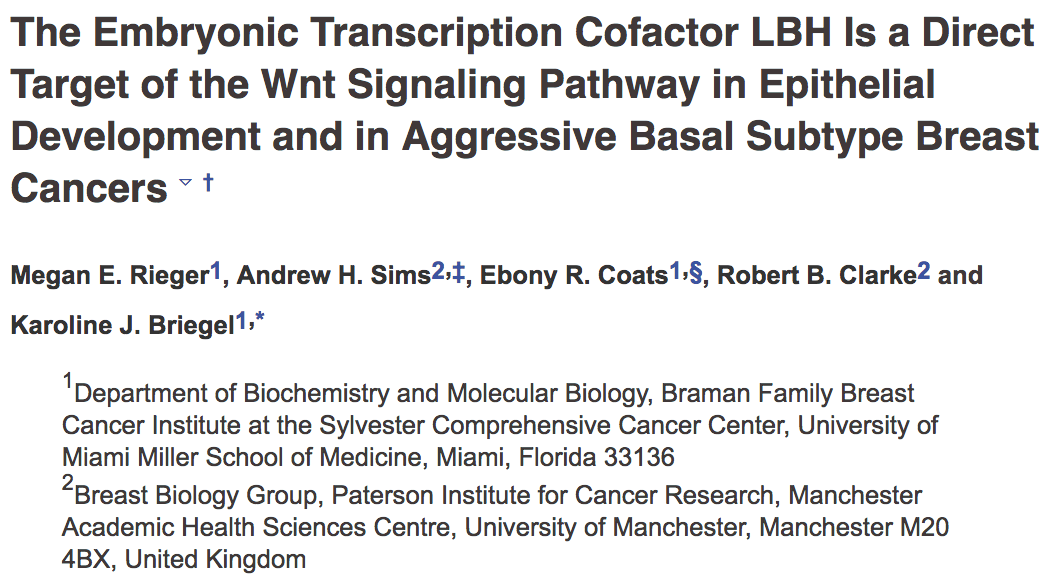
\includegraphics[width=0.8\linewidth]{paper3.png}
% \end{figure}
%\end{frame}

%\begin{frame}{Characterization of chromatin state context of enriched probes using FunciVar}
% \vspace*{-0.3cm}
% \begin{figure}[ht!]
%  \centering
%  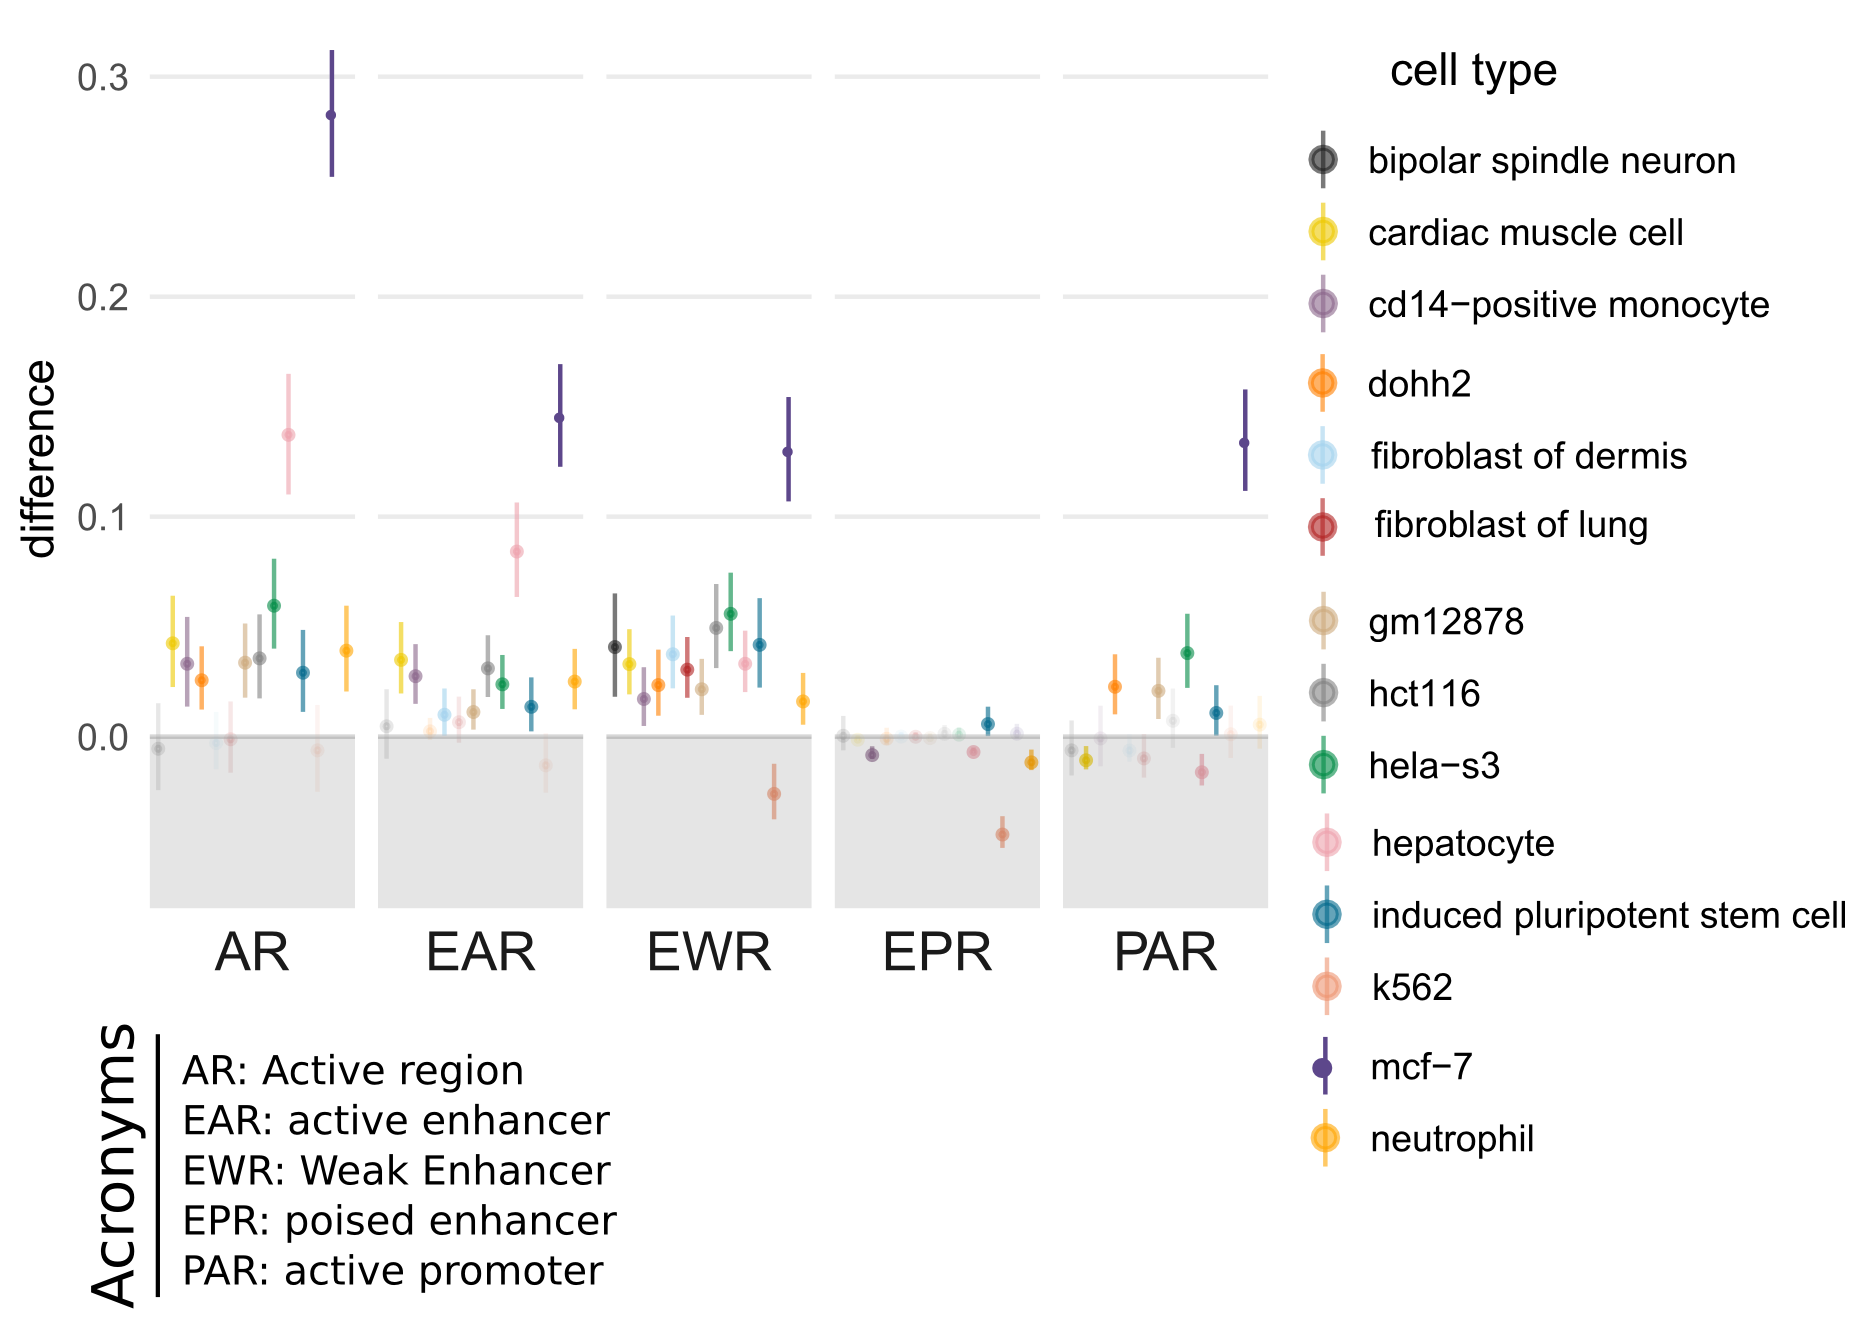
\includegraphics[width=0.9\textwidth]{images/1.png}%\tiny{\\Enrichment of paired probes and chromatin states of encode cells. The plot shows enrichment for enhancer active region (EAR), weak enhancer (EWR) and active promoter region (PAR) for MCF-7 cell. }
 %\end{figure}
%\end{frame}

%\begin{frame}{Comparing inferred results with MCF-7 chIA-PET}

 %\begin{figure}[ht!]
%  \centering
%  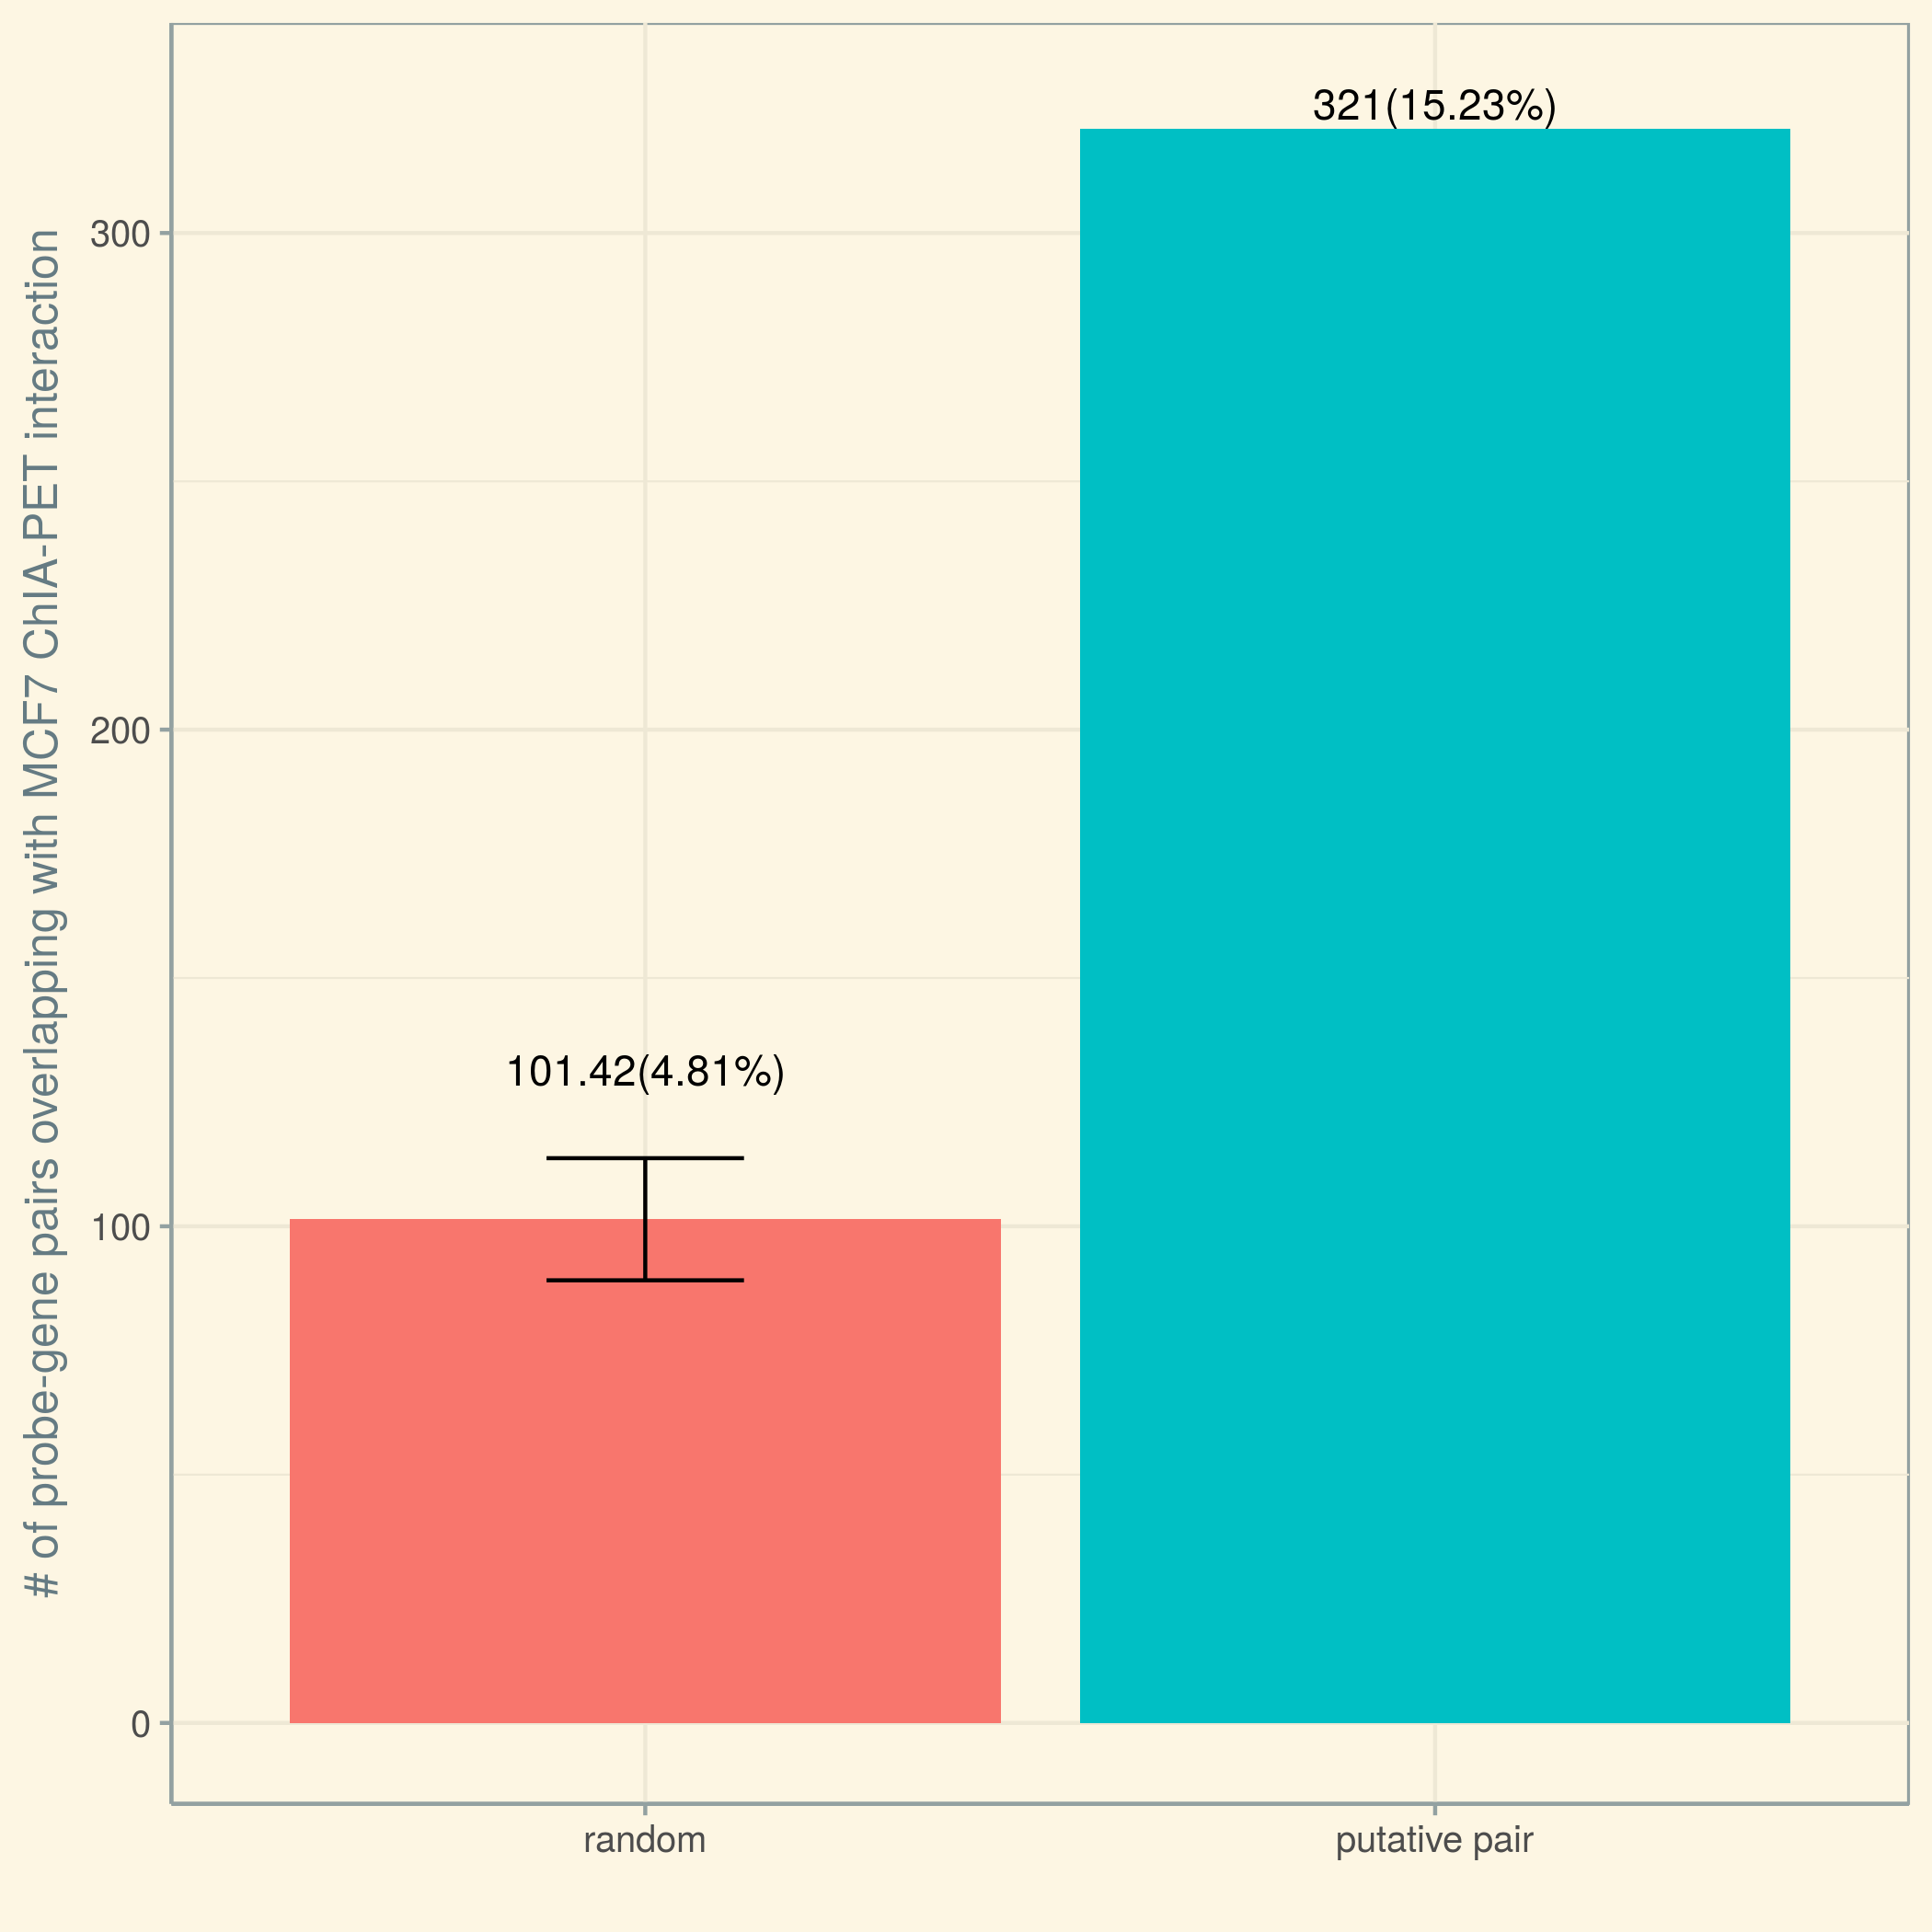
\includegraphics[width=0.6\textwidth]{ELMER/validation.png}\tiny{\\MCF7 ChIA-PET (Chromatin Interaction Analysis with Paired-End-Tag sequencing) from Li, Guoliang, et al. "Extensive promoter-centered chromatin interactions provide a topological basis for transcription regulation." Cell 148.1 (2012): 84-98. (https://doi.org/10.1016/j.cell.2011.12.014).}
% \end{figure}
%\end{frame}

%\begin{frame}[plain]{Supervised analysis: BRCA molecular subtypes}
%\vspace*{-0.45cm}
% \begin{figure}[ht!]
%  \centering
%  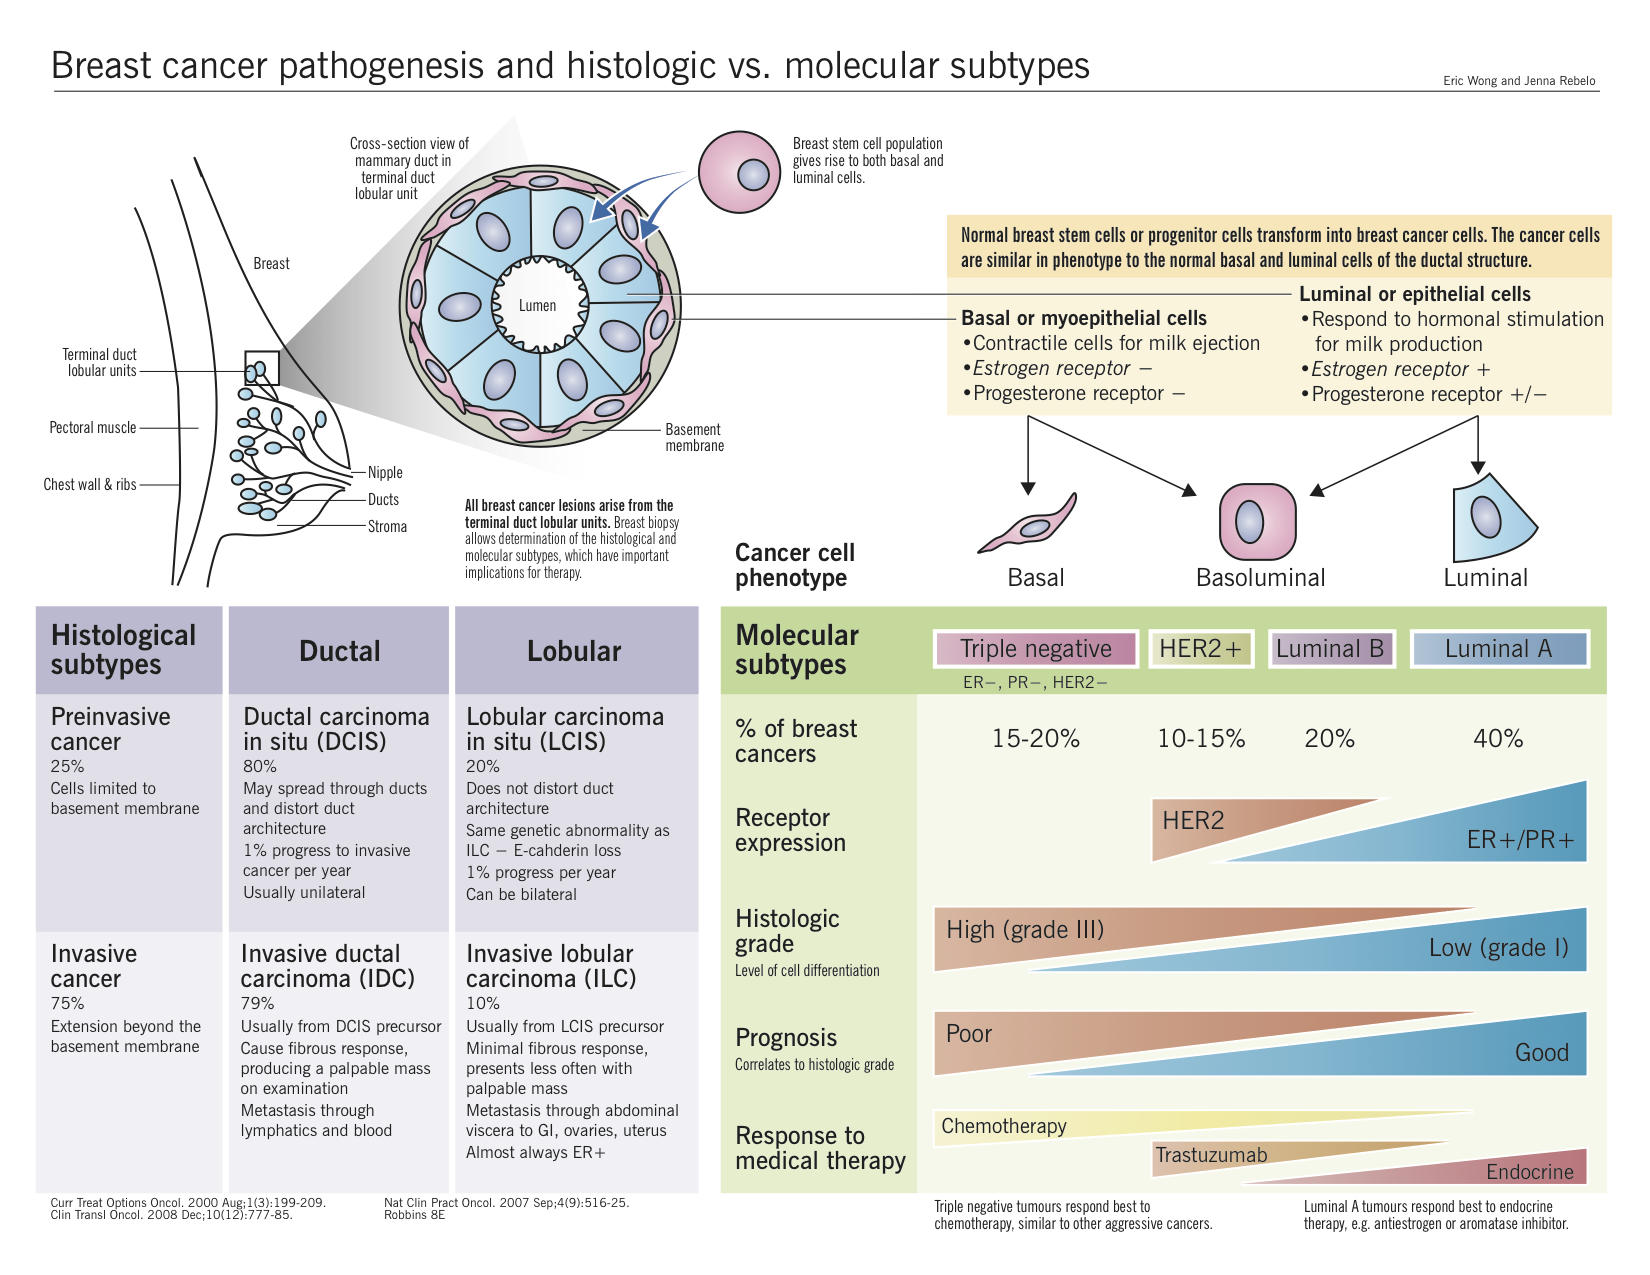
\includegraphics[width=1.0\textwidth]{ELMER/breastcancer-subtypes.png}\tiny{\\Source: Wong ET. Available at: http://www.pathophys.org/breast-cancer/. Accessed 25/12/2017.}
% \end{figure}
% \end{frame}

%\begin{frame}{BRCA supervised analysis}
  %\begin{tabular}{p{2.3cm}p{2.4cm}p{2.4cm}p{1cm}}
   %\toprule
   %Group               & Samples w/ DNA methylation (450K) & Samples w/ gene expression (FPKM-UQ) & Samples w/ both \\ \midrule
   %Primary solid Tumor & 791                               & 1102                                 & 778             \\
   %Solid Tissue Normal & 96                                & 113                                  & 83              \\
   %\bottomrule
  %\end{tabular}
 %\end{table}


 %\begin{figure}[ht!]
  %\centering
%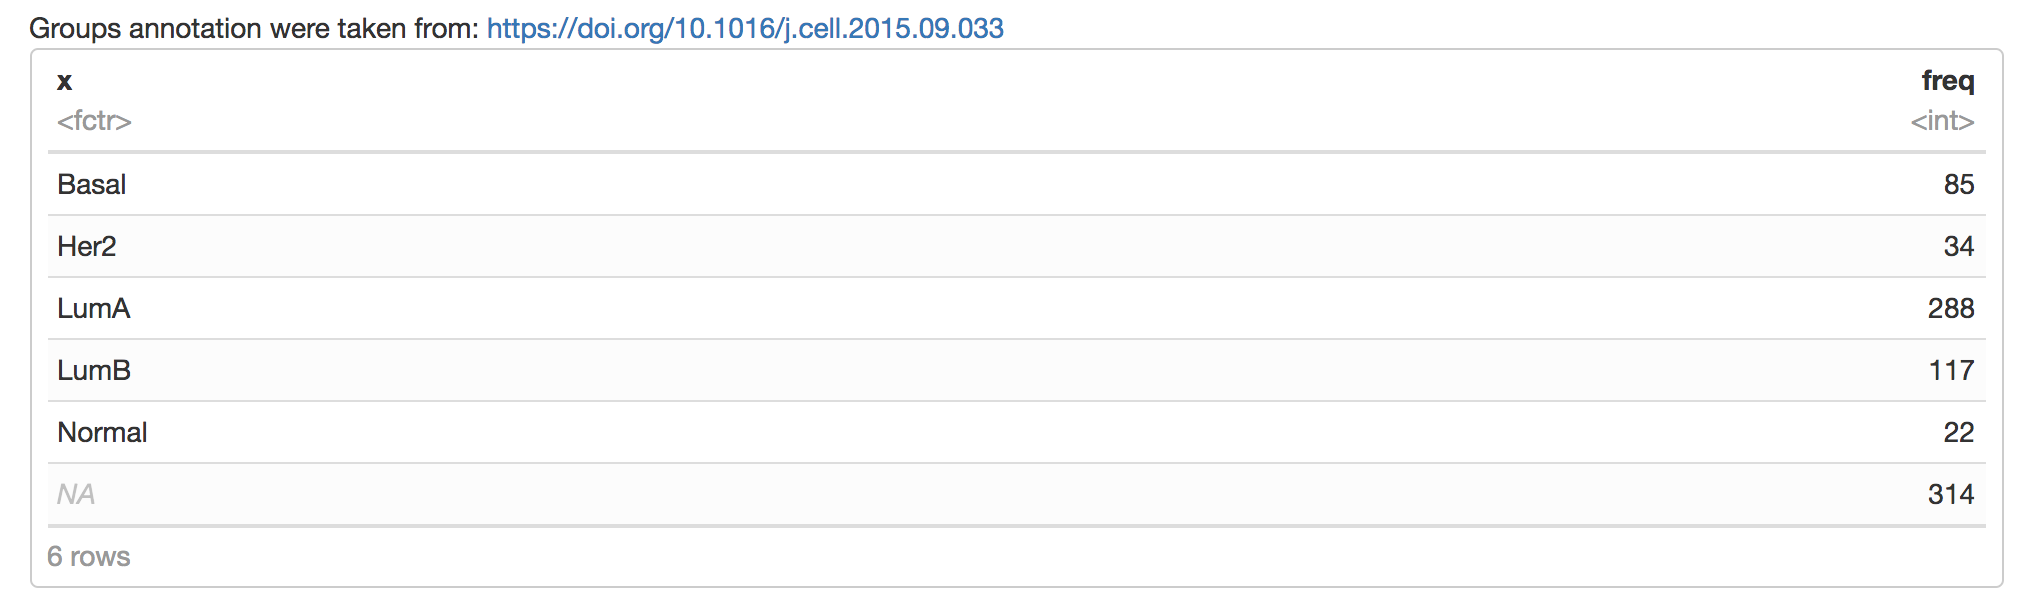
\includegraphics[width=1.0\textwidth]{ELMER/groups.png}
 %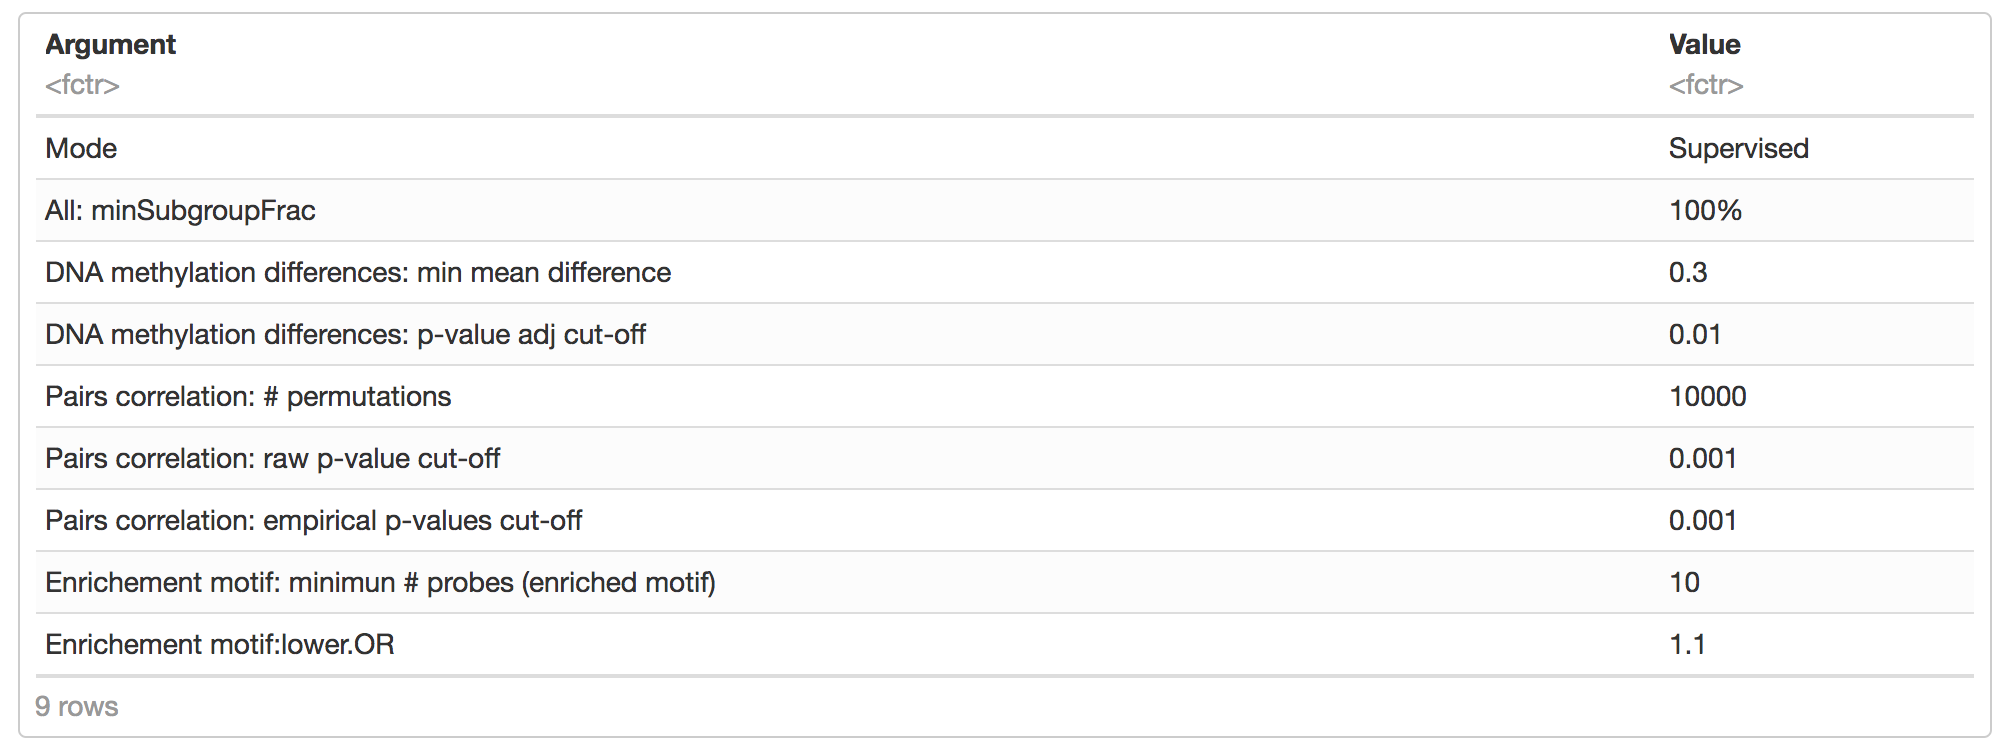
\includegraphics[width=1.0\textwidth]{ELMER/arguments.png}
 %\end{figure}
%\end{frame}

%
\begin{frame}{Candidate master regulator TFs (MRs)}
\vspace*{-0.2cm}
\tiny
\begin{tabular}{@{}|c|c|c|c|c|c|c|c|c|c|@{}}
\hline
\textit{\textbf{TF}} & 
\textbf{\begin{tabular}[c]{@{}c@{}}Tumor \\ (vs Normal)\end{tabular}} &
\textbf{\begin{tabular}[c]{@{}c@{}}LumA \\ (vs basal)\end{tabular}} & \textbf{\begin{tabular}[c]{@{}c@{}}LumB \\ (vs basal)\end{tabular}} & \textbf{\begin{tabular}[c]{@{}c@{}}Basal \\ (vs LumA)\end{tabular}} & \textbf{\begin{tabular}[c]{@{}c@{}}Basal \\ (vs LumB)\end{tabular}} & \textbf{\begin{tabular}[c]{@{}c@{}}Basal \\ (vs HER2)\end{tabular}} & \textbf{\begin{tabular}[c]{@{}c@{}}HER2 \\ (vs Basal)\end{tabular}}   \\ \hline
\textit{\textbf{AR}} & x & x & x &  &  &  &  \\
\textit{\textbf{EMX1}} & x & x & x &  &  &  &  \\
\textit{\textbf{ESR1}} & x & x & x &  &  &  &  \\
\textit{\textbf{GATA3}} & x & x & x &  &  &  &  \\
%\textit{\textbf{HOMEZ}} & x & x & x &  &  &  &  \\
\textit{\textbf{LMX1B}} & x & x & x &  &  &  &  \\
\textit{\textbf{MYB}} & x & x & x &  &  &  &  \\
\textit{\textbf{NR2E3}} & x & x & x &  &  &  &  \\
\textit{\textbf{PATZ1}} & x & x & x &  &  &  &  \\
\textit{\textbf{PBX1}} & x & x & x &  &  &  &  \\
\textit{\textbf{RARA}} & x & x & x &  &  &  &  \\
\textit{\textbf{ZNF467}} & x & x & x &  &  &  &  \\ 
%\textit{\textbf{OVOL2}} & x &  &  &  &  &  &  \\
%\textit{\textbf{ZNF281}} & x &  &  &  &  &  &  \\
\textit{\textbf{FOXD2}} & x &  & x &  &  &  &  \\
%\textit{\textbf{GLI3}} &  & x & x &  &  &  &  \\
%\textit{\textbf{PGR}} &  & x & x &  &  &  &  \\ 
\textit{\textbf{FOXA1}} & x & x & x &  &  &  & x \\ \hline
\textit{\textbf{FOXP1}} &  & x & x &  &  &  & x \\
%\textit{\textbf{HOXB1}} &  & x & x &  &  &  & x \\
\textit{\textbf{HOXB2}} &  & x & x &  &  &  & x \\ \hline
%\textit{\textbf{MSX2}} &  & x & x &  &  &  & x \\ \hline
\textit{\textbf{HOXB3}} &  &  &  &  &  &  & x \\
%\textit{\textbf{HOXB6}} &  &  &  &  &  &  & x \\
\textit{\textbf{HOXC10}} &  &  &  &  &  &  & x \\
%\textit{\textbf{HOXC11}} &  &  &  &  &  &  & x \\
\textit{\textbf{MNX1}} &  &  &  &  &  &  & x \\
\textit{\textbf{NKX2-2}} &  &  &  &  &  &  & x \\ \hline
\textit{\textbf{BCL11A}} &  &  &  & x & x & x &  \\
\textit{\textbf{ELF5}} &  &  &  & x & x & x &  \\
\textit{\textbf{ETV6}} &  &  &  & x & x & x &  \\
%\textit{\textbf{ZIC1}} &  &  &  & x & x & x &  \\
\textit{\textbf{CEBPB}} &  &  &  & x & x &  &  \\
\textit{\textbf{NFIB}} &  &  &  & x & x &  &  \\
%\textit{\textbf{NFIL3}} &  &  &  & x & x &  &  \\
\textit{\textbf{RUNX3}} &  &  &  & x & x &  &  \\
\textit{\textbf{SOX11}} &  &  &  & x & x &  &  \\
\textit{\textbf{E2F3}} &  &  &  &  & x & x &  \\
\textit{\textbf{KLF5}} &  &  &  &  & x & x &  \\
%\textit{\textbf{SOX8}} &  &  &  &  & x & x &  \\
\textit{\textbf{SOX9}} &  &  &  &  & x & x &  \\ \hline
\end{tabular}
\end{frame}




%\begin{frame}{TF master regulator: LumA}

% \begin{figure}[ht!]
%  \centering
%  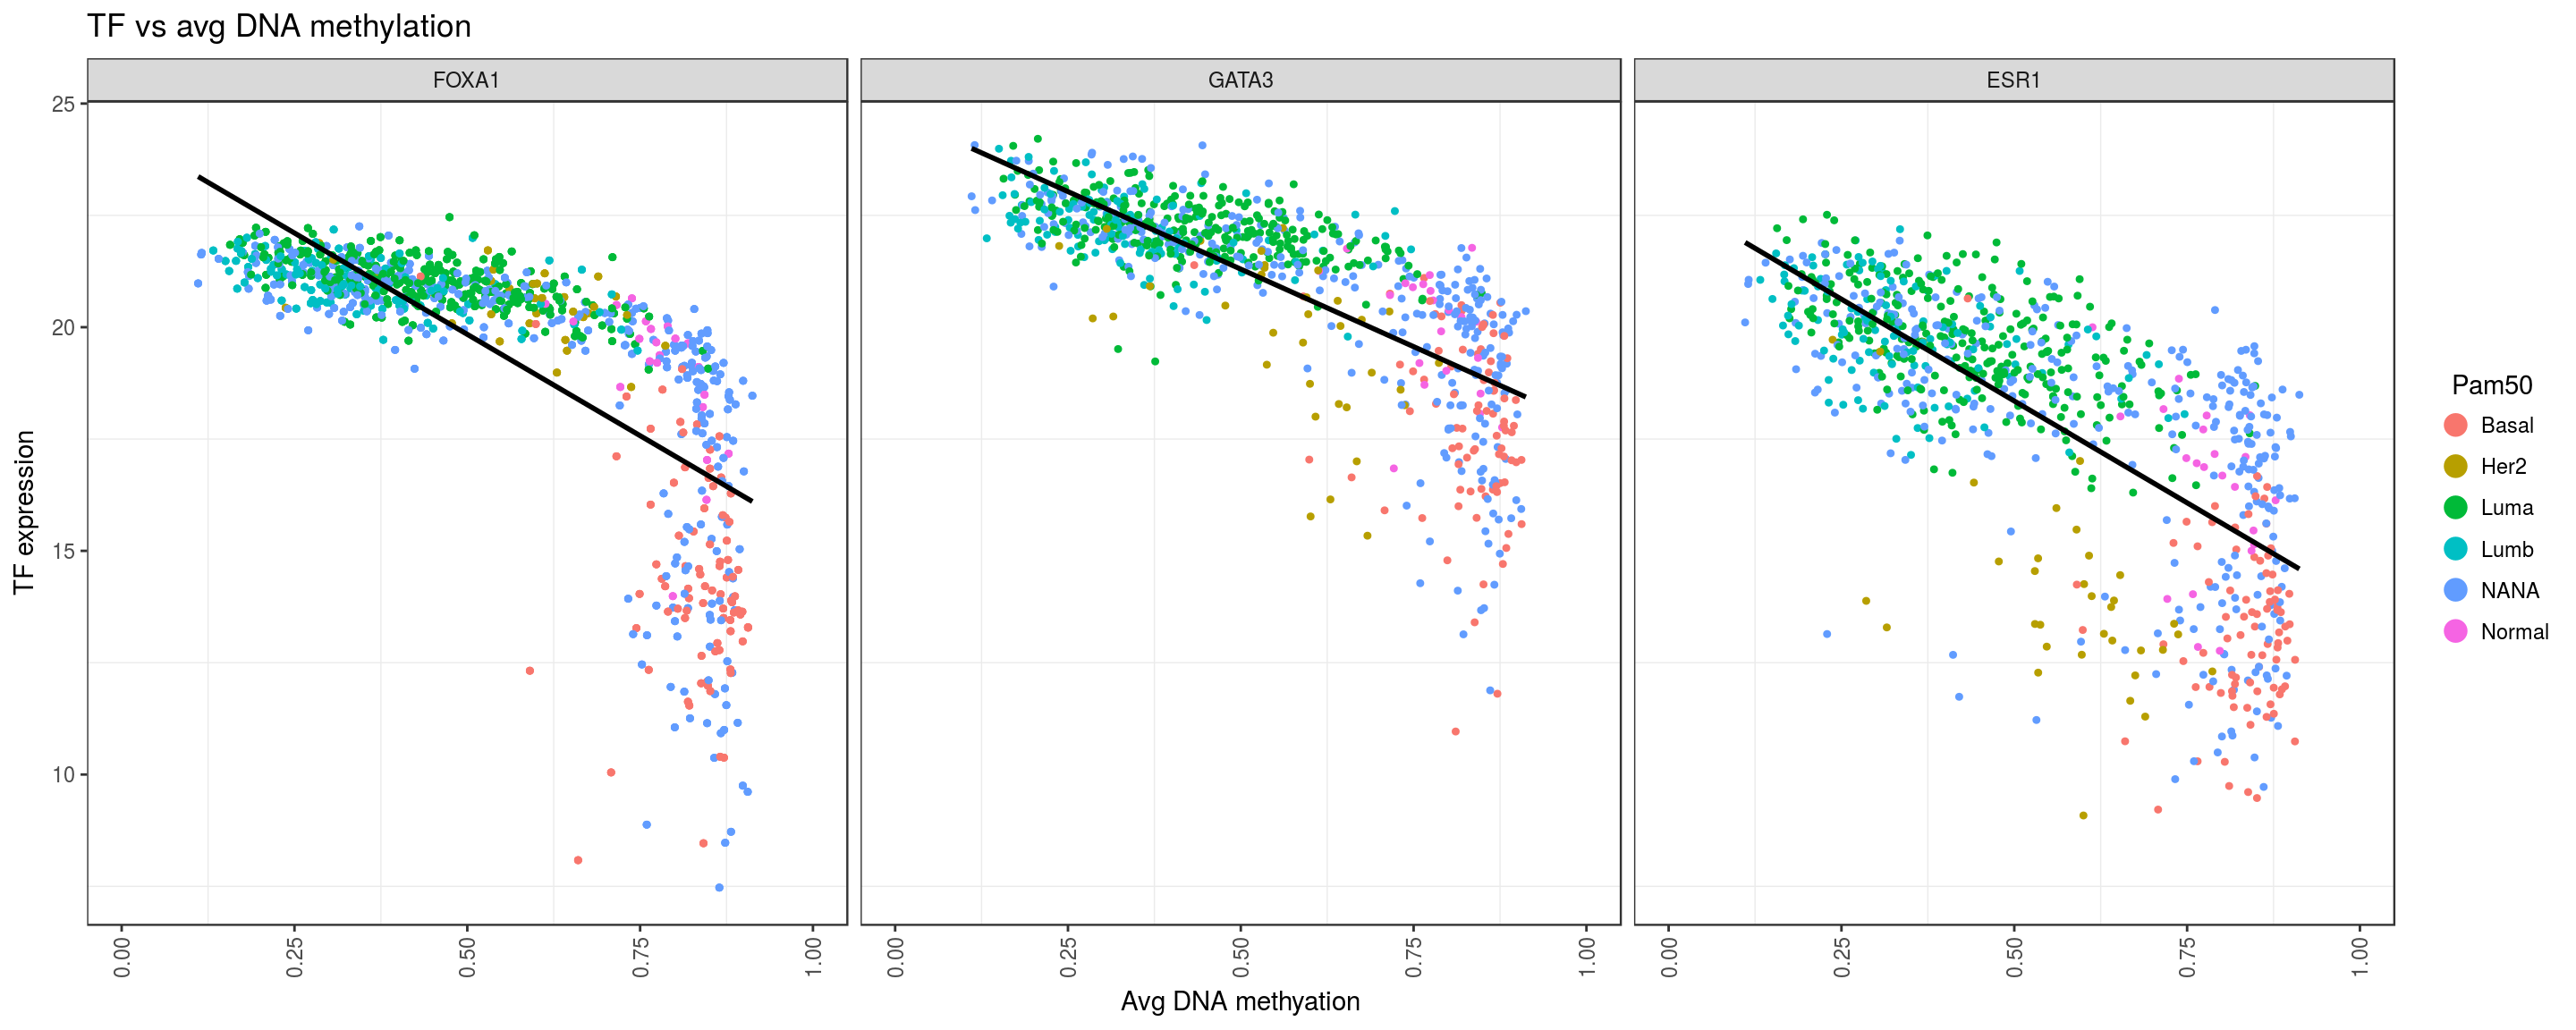
\includegraphics[width=1.0\textwidth]{ELMER/FOXA3_motif.png}
%  \caption{\label{fig:chiapet} FOXA1 and top3 TF expression vs avg DNA methylation of paired enriched probes for FOXA3 motif - Probes hypomethylated in LumA vs Normal-like}
% \end{figure}
%\end{frame}

%\begin{frame}{TF master regulator: Basal}
% \begin{figure}[ht!]
%  \centering
%  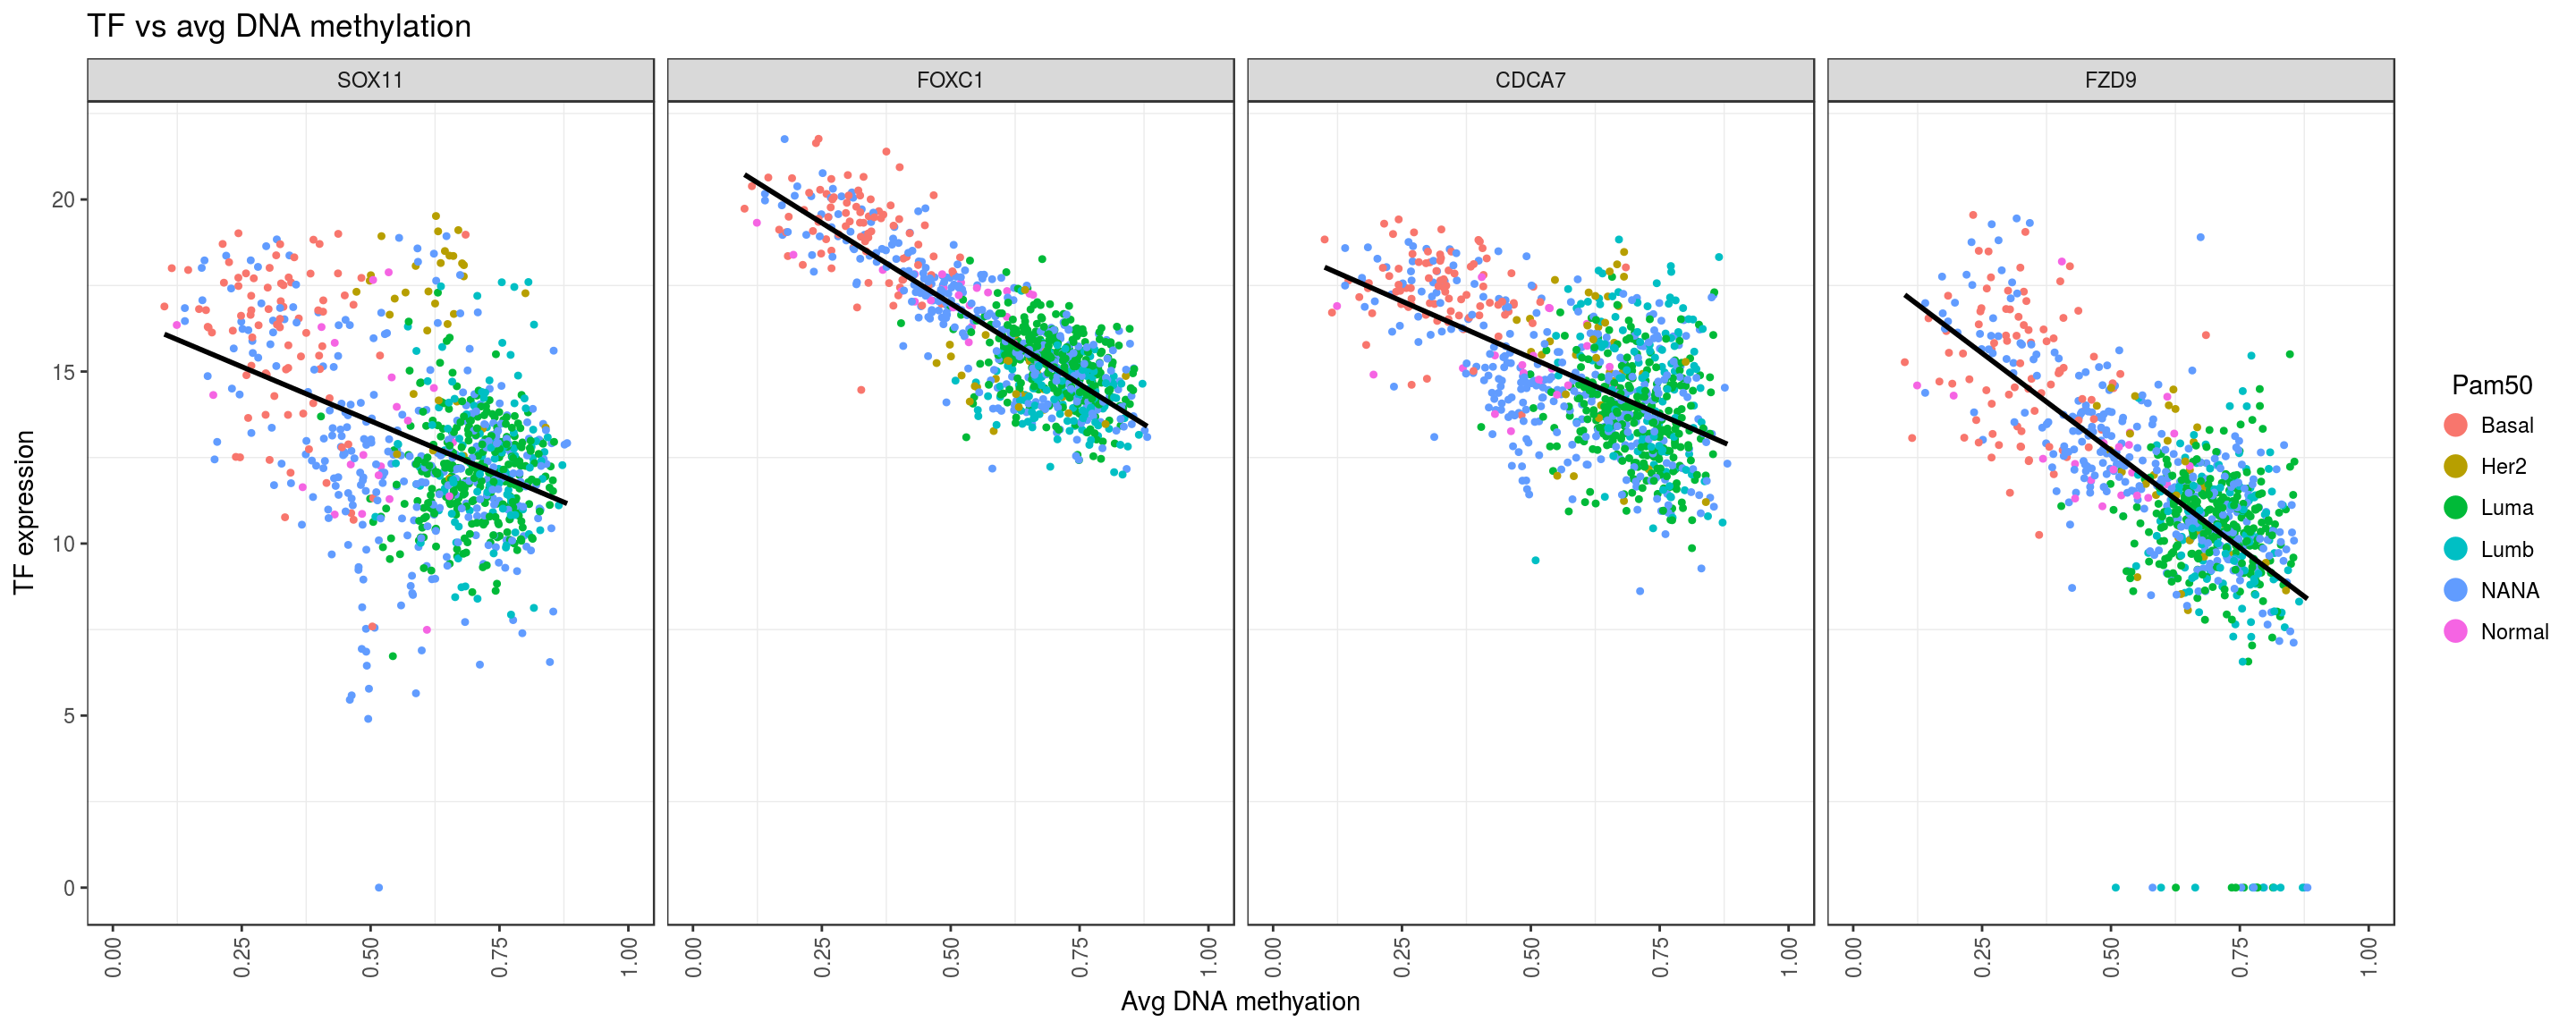
\includegraphics[width=1.0\textwidth]{ELMER/SOX10_TF.png}
%  \caption{\label{fig:chiapet} SOX11 and top3 TF expression vs avg DNA methylation of paired enriched probes for SOX10 - Probes hypermethylated in LumA vs Basal}
% \end{figure}
%\end{frame}


\begin{frame}{Master regulator TF: molecular known subtypes}

 \begin{figure}[ht!]
  \centering
  
\includegraphics[width=1.0\textwidth]{ELMER/SOX11_basal.png}
  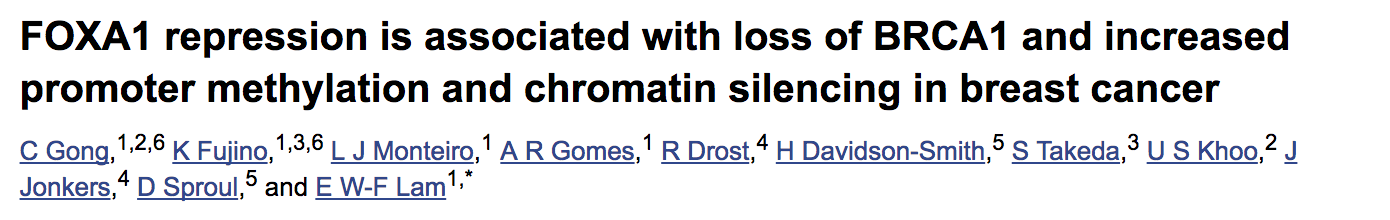
\includegraphics[width=1.0\textwidth]{ELMER/SOX9_2.png}
  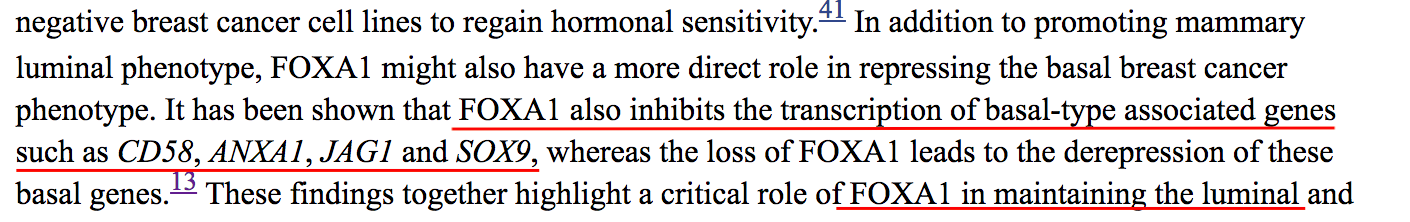
\includegraphics[width=1.0\textwidth]{ELMER/SOX9_1.png}
  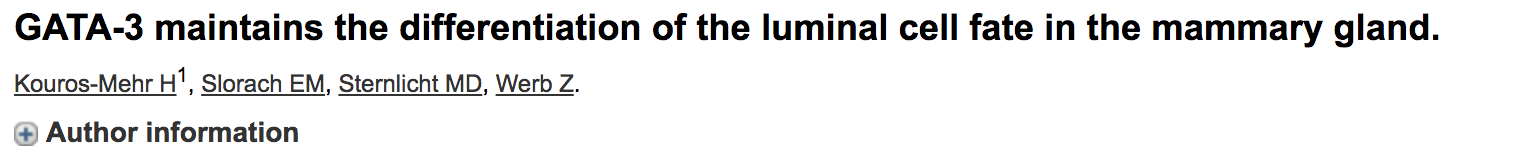
\includegraphics[width=1.0\textwidth]{ELMER/GATA3.png}
  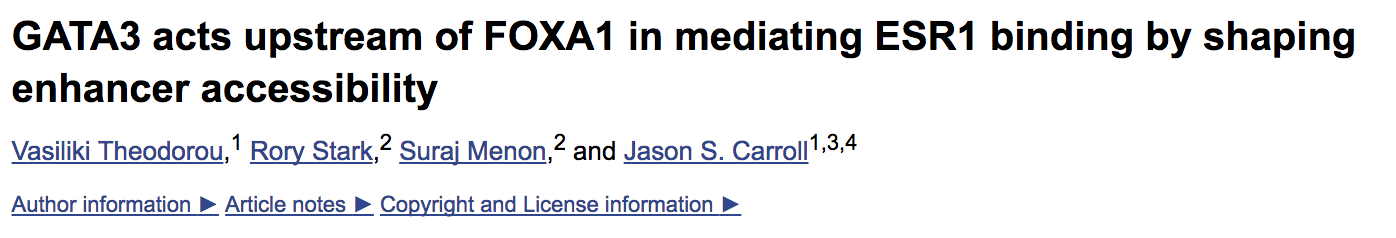
\includegraphics[width=1.0\textwidth]{ELMER/cofactors.png}
     \end{figure}
\end{frame}

\begin{frame}{Next steps: TF knockdown}
 \begin{figure}[ht!]
  \centering
  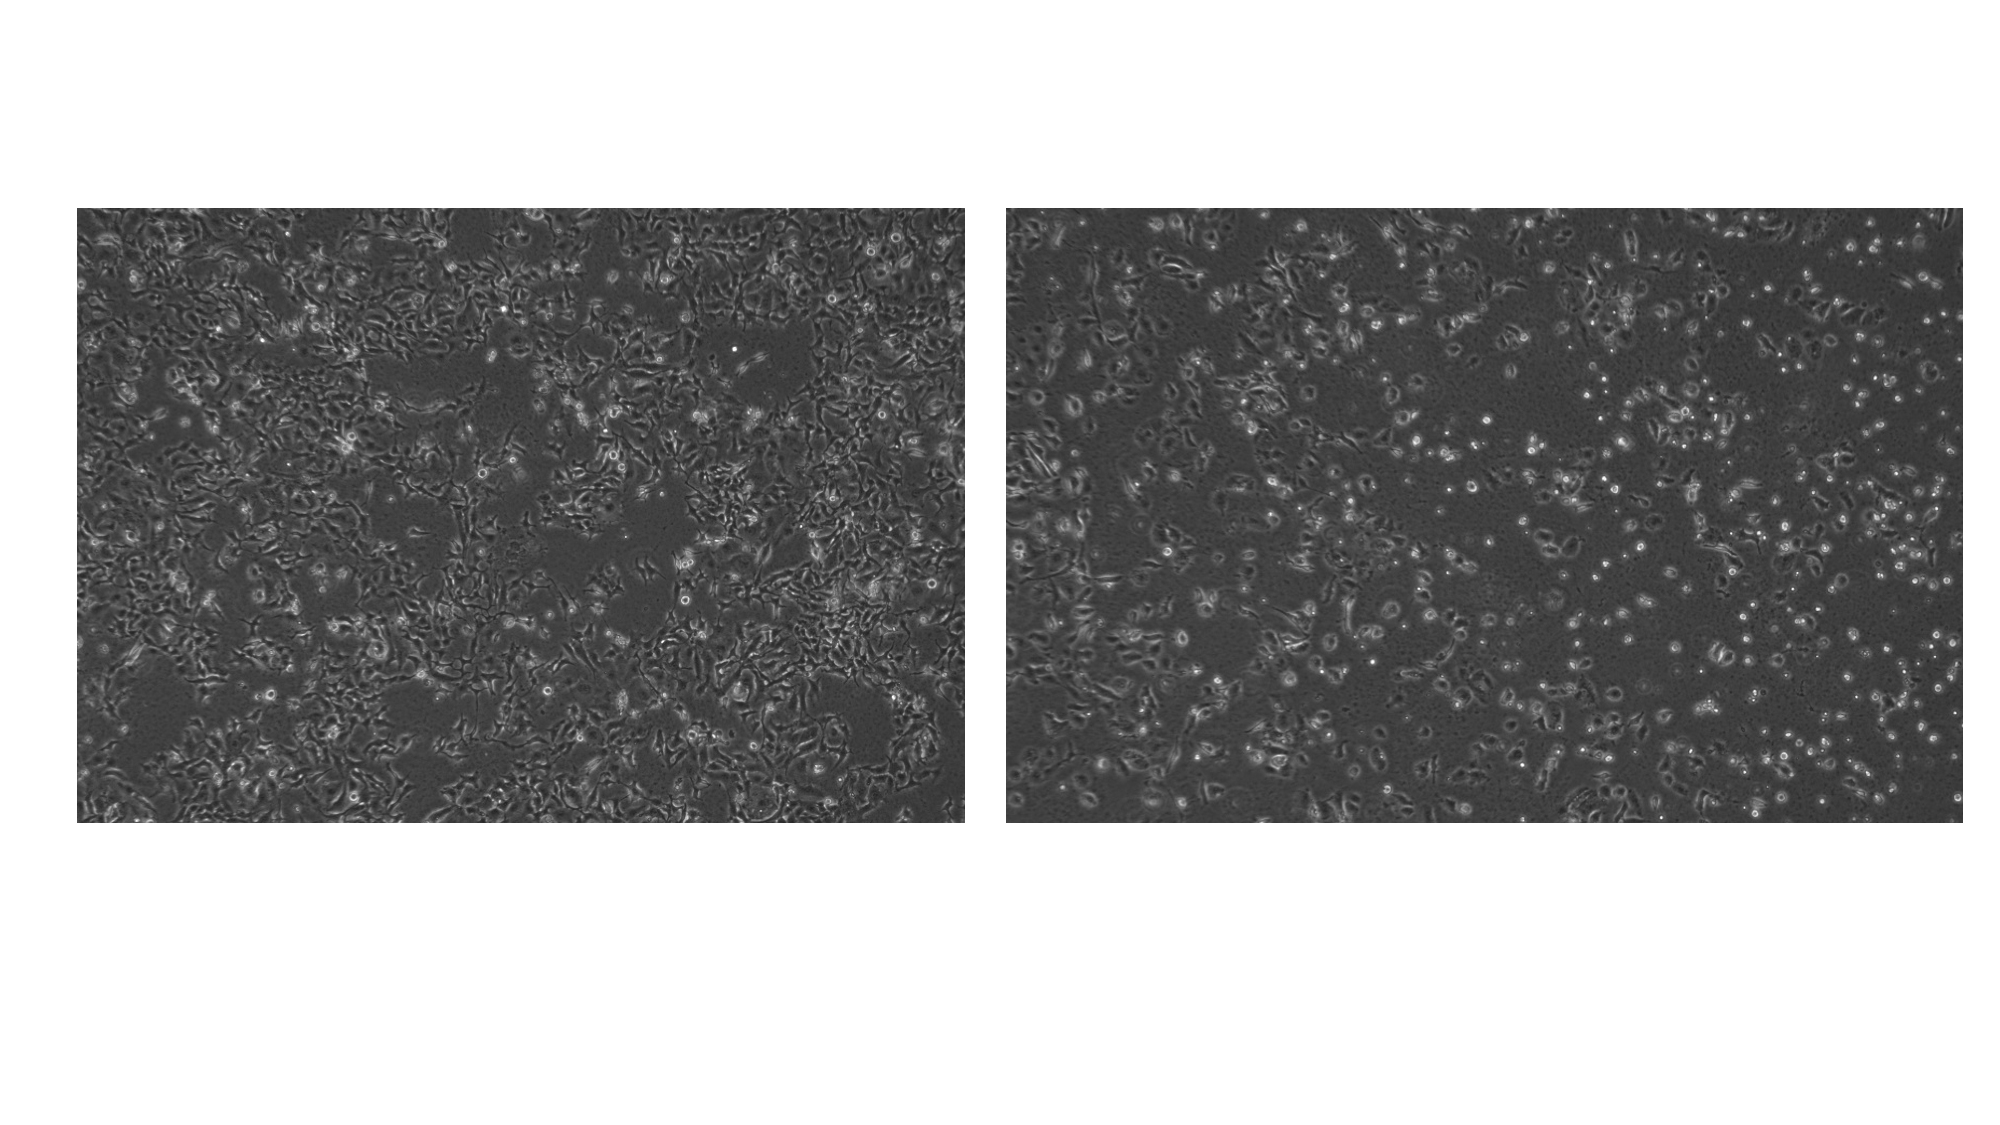
\includegraphics[width=1.0\textwidth]{glioma/knockdown_TF_ESCA.pdf}
  \caption{Candidate master regulator Transcription Factors (TF) knockdown in the SKGT4 human esophageal adenocarcinoma cell line. Figure produced by Dr. Dechen Lin.}
 \end{figure}
\end{frame}


%\begin{frame}[plain]%{Workflow}
 %\vspace*{-0.3cm}
 %\hspace*{-0.3cm}
% \begin{figure}
%  \hspace*{-1cm}
 %\centering
%  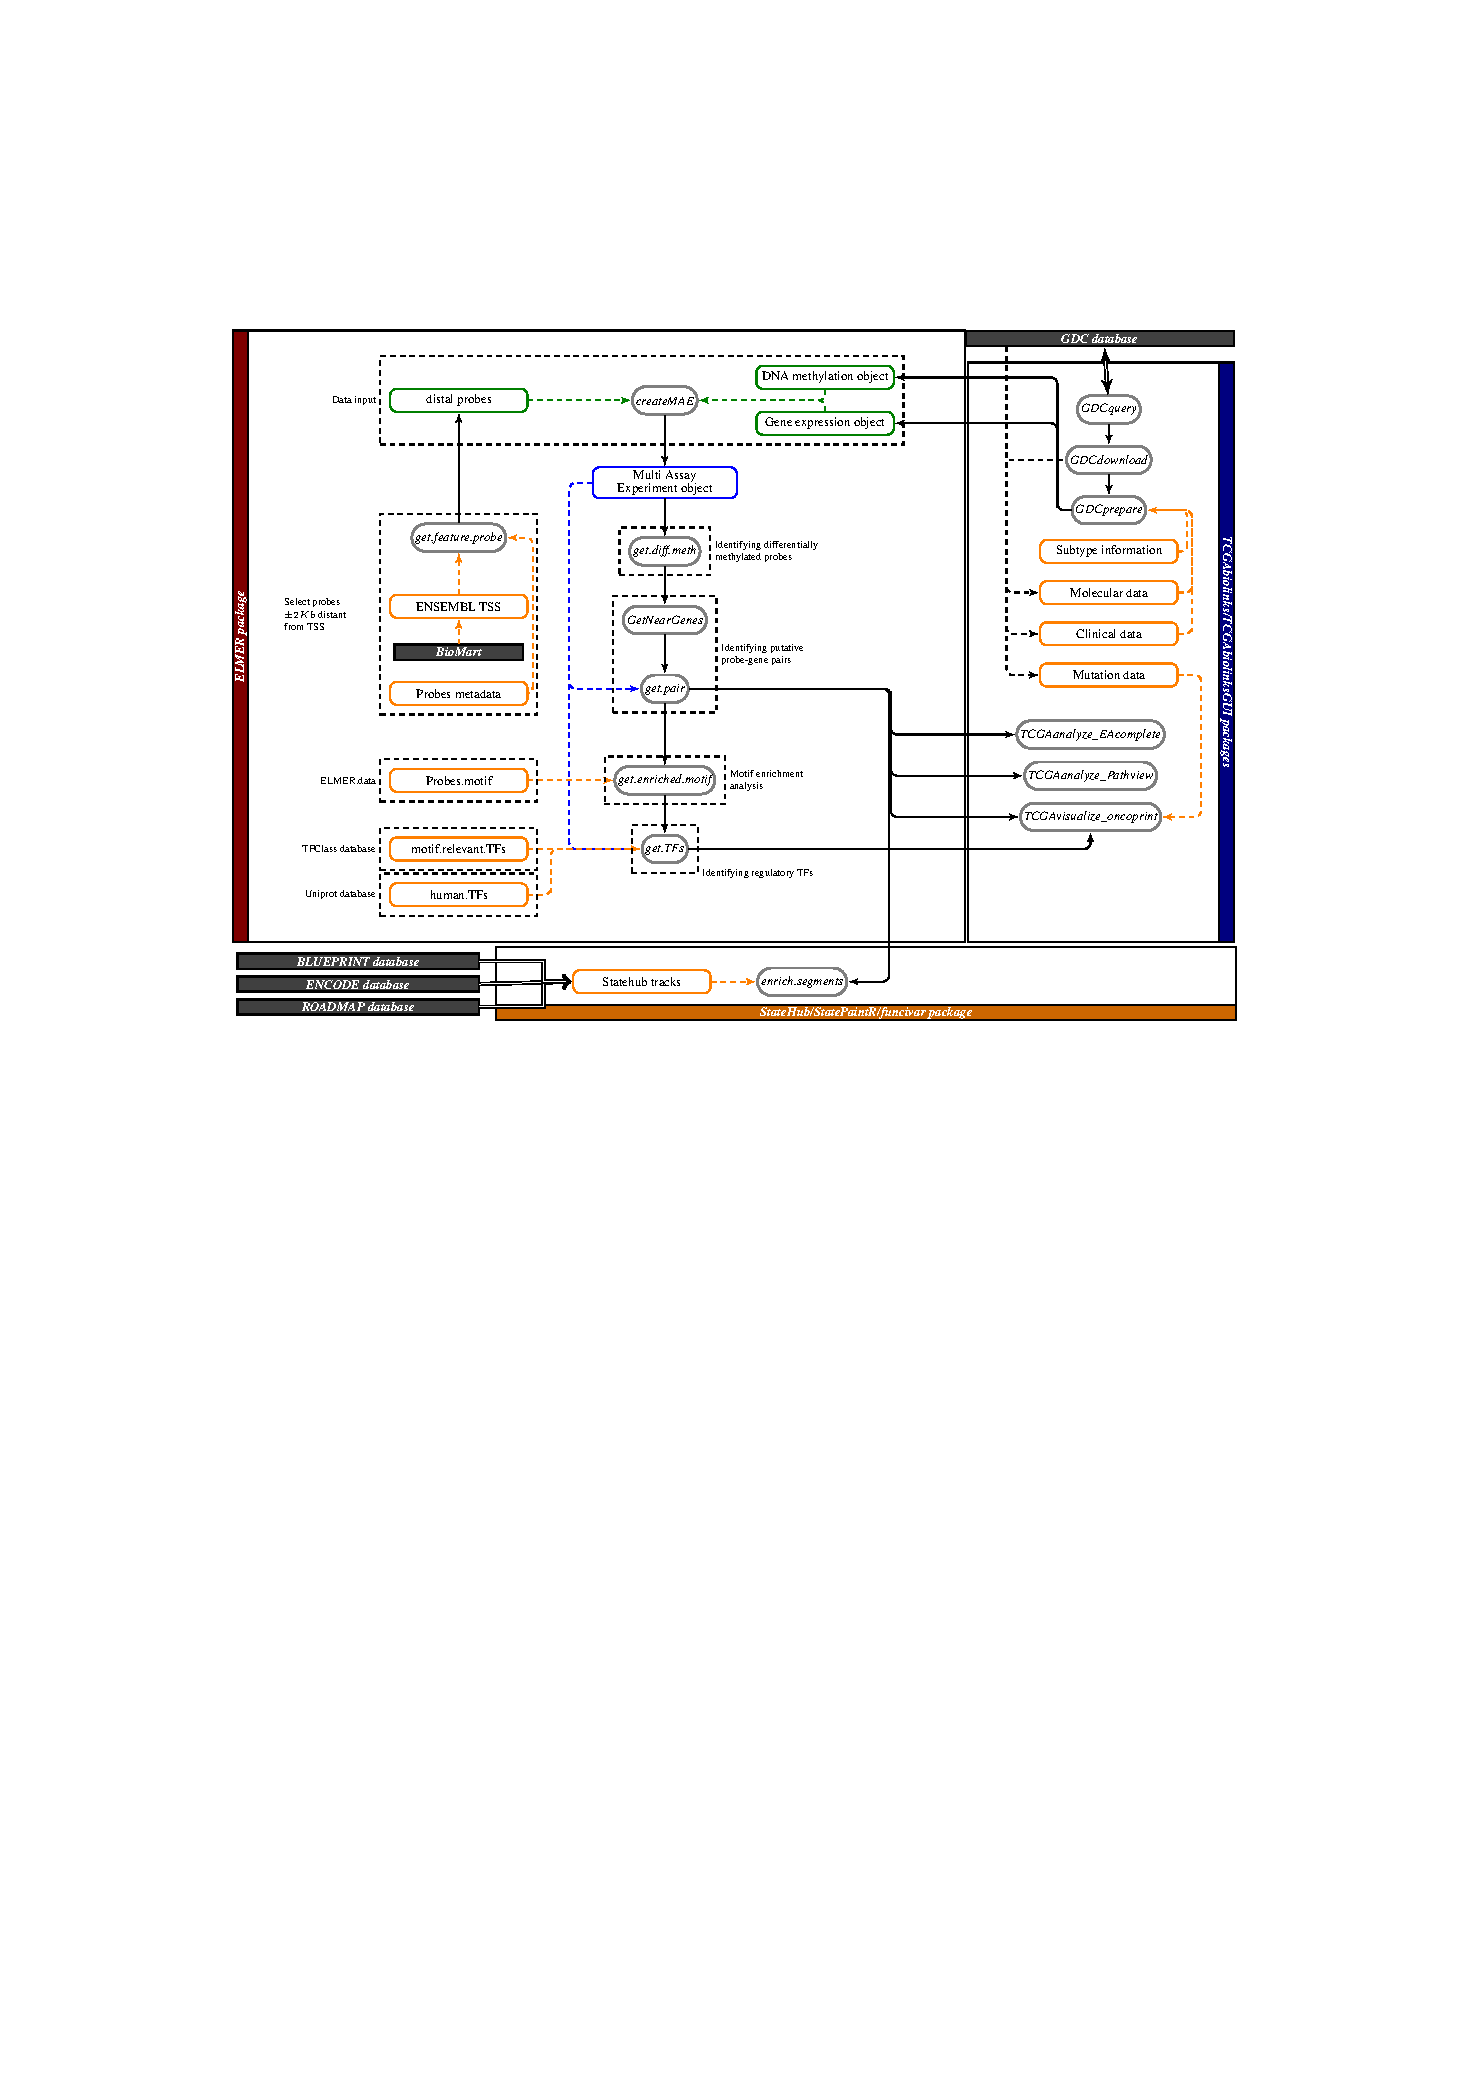
\includegraphics[width=1.18\linewidth]{ELMER/workflow_new.pdf}
% \end{figure}
%\end{frame}


\end{document}
